\chapter{Apendice}
\label{apendice}
\section{Estudo da bibliografia}

Este arquivo serve para fazer apontamentos acerca da bibliografia indicada/pesquisada.

\subsection{Estudo do artigo~\cite{lee}}

A matriz de espalhamento complexa {\boldmath S} é definida por
$$
\mathbf{ s} = \left[
\begin{array}{cc}
	S_{hh}   & S_{hv}   \\
	S_{vh}   & S_{vv}   \\
\end{array}
\right].
$$
% % % ACF Dizer o que significam "h" e "v"

Usaremos o caso do meio de propagação ser recíproco, isto é, $S_{hv}=S_{vh}$ tornando a matriz de espalhamento simétrica. Podemos facilitar a notação representando a matriz de espalhamento por um vetor da seguinte forma
$$
\mathbf{s} = \left[
\begin{array}{c}
	S_{vv}      \\
	S_{vh}     \\
	S_{hh}      \\
\end{array}
\right].
$$
% % % ACF Não é sempre um fato. Ocorre na maioria das vezes, e em português é "meio recíproco".

De acordo com \cite{good} a distribuição gaussiana complexa multivariada pode modelar adequadamente o comportamento estatístico de $\boldmath S$. Isto é chamado de {\it single-look complex PolSAR data representation} e podemos definir o vetor de espalhamento por $\mathbf{s}=[S_1,S_2,\dots,S_p]^T$. 
% % % ACF Acrescentei "complex"

A função densidade de probabilidade ({\boldmath pdf}) da distribuição gaussiana complexa $p-$variada é dada por
\begin{equation}\label{eqn1}
	p(\mathbf{s})=\frac{1}{\pi^p|\Sigma_{\mathbf{s}}|}\exp(-\bar{\mathbf{s}}^{T}\Sigma_{\mathbf{s}}^{-1}\mathbf{s}).
\end{equation}
O parâmetro que indexa a distribuição é a matriz de covariância, que é definida por:
\begin{equation}\label{eqn2}
	\mathbf{ \Sigma_{s}} = E[\mathbf{ss}^H] = \left[
\begin{array}{cccc}
	E(\mathbf{s_1s_1}^H)  & E(\mathbf{s_1s_2}^H) &\hdots & E({\mathbf s_1s_p}^H) \\
	E(\mathbf{ s_2s_1}^H)  & E(\mathbf {s_2 s_2}^H) &\hdots &E(\mathbf {s_2 s_p}^H)\\
        \vdots&\vdots &\ddots &\vdots\\
	E(\mathbf{ s_ps_1}^H)  & E(\mathbf {s_ps_2}^H) &\hdots &E(\mathbf {s_ps_p}^H)\\
\end{array}
\right].
\end{equation}
onde $E(\cdot)$ e $(\cdot)^H$ denotam o valor esperado e o conjugado transposto.

A matriz {\boldmath$\Sigma_{\mathbf{s}}$} é hermitiana pois se $\mathbf {S_j}= x_j+iy_j $

\begin{equation}\label{eqn3}
\begin{array}{ccc}
\mathbf{S}_j\overline{\mathbf{S}}_j&=& (x_j+iy_j)\overline{(x_j+iy_j)} \\
\mathbf{S}_j\overline{\mathbf{S}}_j&=& (x_j+iy_j)(x_j-iy_j) \\
\mathbf{S}_j\overline{\mathbf{S}}_j&=& x_j^2+y_j^2 \\
\end{array}
\end{equation}
considerando $j \neq k$
\begin{equation}\label{eqn4}
\begin{array}{ccc}
\mathbf{S}_j\overline{\mathbf{S}}_k&=& (x_j+iy_j)\overline{(x_k+iy_k)} \\
\mathbf{S}_j\overline{\mathbf{S}}_k&=& (x_j+iy_j)(x_k-iy_k) \\
\mathbf{S}_j\overline{\mathbf{S}}_k&=& (x_jx_k+y_jy_k)+i(x_ky_j-x_jy_k) \\
\end{array}
\end{equation}
ainda,
\begin{equation}\label{eqn5}
\begin{array}{ccc}
	\overline{\mathbf{S}_k\overline{\mathbf{S}}}_j&=&\overline{ (x_k+iy_k)\overline{(x_j+iy_j)} }\\
	\overline{\mathbf{S}_k\overline{\mathbf{S}}}_j&=&\overline{ (x_k+iy_k)(x_j-iy_j)} \\
	\overline{\mathbf{S}_k\overline{\mathbf{S}}}_j&=&\overline{ (x_kx_j+y_ky_j)+i(x_jy_k-x_ky_j) }\\
	\overline{\mathbf{S}_k\overline{\mathbf{S}}}_j&=&(x_kx_j+y_ky_j)-i(x_jy_k-x_ky_j) \\
	\overline{\mathbf{S}_k\overline{\mathbf{S}}}_j&=&(x_kx_j+y_ky_j)+i(x_ky_j-x_jy_k) \\
\end{array}
\end{equation}
Portanto
\begin{equation}\label{eqn6}
\begin{array}{ccc}
	\mathbf{S}_j\overline{\mathbf{S}}_j&=&\overline{\mathbf{S}_j\overline{\mathbf {S}}}_j \\
	\mathbf{S}_j\overline{\mathbf{S}}_k&=&\overline{\mathbf{S}_k\overline{\mathbf {S}}}_j \\
\end{array}
\end{equation}
Assim com $j$ e $k$ varrendo toda a matriz podemos afirmar que $\mathbf{\Sigma_{\mathbf{s}}}=\mathbf{\Sigma_{ s}}^H$ portanto hermitiana.


Dados polarimétricos são usualmente sujeitados a um processo {\it multilook} com o intuito de melhorar a razão sinal-ruído.
% % % ACF "relação senhal-ruído"
Para esse fim, matrizes positivas definidas hermitianas são obtidas computando a médias de $L$ visadas 
% % % ACF "visadas", mas ninguém usa
independentes de uma mesma cena. Isto resulta na matriz de covariância {\boldmath{Z}} dada por:
\begin{equation}\label{eqn7}
	\mathbf{Z}=\frac{1}{L}\sum_{i=1}^{L} \mathbf{s_is_i}^H .
\end{equation}
% % % ACF Código LaTeX simplificado

\subsubsection{Coeficiente de correlação {\it Multilook}}

O coeficiente de correlação complexo é um importante parâmetro para descrever a função de densidade de probabilidade. 
Podemos defini-lo como
\begin{equation}\label{eqn8}
	\rho_c=\frac{E[\mathbf{s_is_j}^H]}{\sqrt{E[|\mathbf{s_i}|^2]E[|\mathbf{s_j}|^2]}} =|\rho_c|e^{i\theta}.
\end{equation}
% % % ACF Não complique LaTeX
em que {\boldmath $s_i$} e {\boldmath $s_j$} 
% % % ACF Repare que o negrito matemático se faz de outra maneira
são duas componentes da matriz de espalhamento ou dois retorno do radar polarimétrico ou interferométrico SAR. 
Para dados de radar polarimétricos representado pela matriz de Mueller, $\rho_c$ pode ser calculado encontrando a média da vizinhança de um pixel de uma matriz Mueller. A magnitude de $\rho_c$ pode também ser estimada usando duas intensidade  {\it multilook} $Z_{ii}$ e $Z_{jj}$. O coeficiente de correlação de dados $L$ looks intensidade é definida como   
% % % ACF Eram L looks, agora são n. Unificar a notação
\begin{equation}\label{eqn9}
	\rho_I^{(n)}=\frac{E[(Z_{ii}-\overline{Z_{ii}})(Z_{jj}-\overline{Z_{jj}})]}{\sqrt{E[(Z_{ii}-\overline{Z_{ii}})^2][(Z_{jj}-\overline{Z_{jj}})^2]}}. \\
\end{equation}

No apêndice do artigo \cite{lee} foi mostrado que 

\begin{equation}\label{eqn10}
	\rho_I^{(n)}= |\rho_c|^2\\
\end{equation}

Sendo 

\begin{equation}\label{eqn11}
\begin{array}{ccc}
	\mathbf{S_i}&=&a_{R}+ia_{I} \\
        \mathbf{S_j}&=&b_{R}+ib_{I} \\
\end{array}
\end{equation}

Assim a equação (\ref{eqn8}) pode ser reescrita

\begin{equation}\label{eqn12}
\begin{array}{ccc}
	\rho_c&=&\frac{E[(a_{R}+ia_{I})\overline{(b_{R}+ib_{I})}]}{\sqrt{E[a_{R}^2+a_{I}^2]E[b_{R}^2+b_{I}^2]}}. \\
	\rho_c&=&\frac{E[(a_{R}+ia_{I})(b_{R}-ib_{I})]}{\sqrt{E[a_{R}^2+a_{I}^2]E[b_{R}^2+b_{I}^2]}}. \\
	\rho_c&=&\frac{E[a_{R}b_{R}+ia_{I}b_{R}-ia_{R}b_{I}+a_{I}b_{I}]}{\sqrt{E[a_{R}^2+a_{I}^2]}\sqrt{E[b_{R}^2+b_{I}^2]}}. \\
	\rho_c&=&\frac{E[a_{R}b_{R}+ia_{I}b_{R}-ia_{R}b_{I}+a_{I}b_{I}]}{\sqrt{E[a_{R}^2+a_{I}^2]}\sqrt{E[b_{R}^2+b_{I}^2]}}. \\
\end{array}
\end{equation}
Definindo os desvios padrões,
\begin{equation}\label{eqn13}
\begin{array}{ccc}
	\sigma_{a}	&=&\sqrt{E[a_{R}^2+a_{I}^2]} \\
	\sigma_{b}      &=&\sqrt{E[b_{R}^2+b_{I}^2]} \\
\end{array}
\end{equation}

\begin{equation}\label{eqn14}
\begin{array}{ccc}
	\rho_c&=&\frac{E[a_{R}b_{R}+ia_{I}b_{R}-ia_{R}b_{I}+a_{I}b_{I}]}{\sigma_a\sigma_b}. \\
	\rho_c&=&\frac{E[a_{R}b_{R}+a_{I}b_{I}+i(a_{I}b_{R}-a_{R}b_{I})]}{\sigma_a\sigma_b}. \\
	\rho_c&=&\frac{E[a_{R}b_{R}]+E[a_{I}b_{I}]+i(E[a_{I}b_{R}]-E[a_{R}b_{I})]}{\sigma_a\sigma_b}. \\
	\rho_c&=&\frac{E[a_{R}b_{R}]}{\sigma_a\sigma_b}+\frac{E[a_{I}b_{I}]}{\sigma_a\sigma_b}+i\left(\frac{E[a_{I}b_{R}]}{\sigma_a\sigma_b}-\frac{E[a_{R}b_{I}]}{\sigma_a\sigma_b}\right). \\
\end{array}
\end{equation}
Definindo
\begin{equation}\label{eqn15}
\begin{array}{ccccccccc}
	\rho_{RR}=\frac{E[a_{R}b_{R}]}{\sigma_a\sigma_b},&&\rho_{II}=\frac{E[a_{I}b_{I}]}{\sigma_a\sigma_b},&&\rho_{IR}=\frac{E[a_{I}b_{R}]}{\sigma_a\sigma_b},&&\rho_{RI}=\frac{E[a_{R}b_{I}]}{\sigma_a\sigma_b}. \\
\end{array}
\end{equation}

Portanto, 
\begin{equation}\label{eqn16}
	\rho_c=\frac{(\rho_{RR}+\rho_{II})+i(\rho_{IR}-\rho_{RI})}{2}. \\
\end{equation}

\textcolor{red}{obs:Explicar melhor o fator 2}

Devido a condição de ser gaussiana circular

\begin{equation}\label{eqn17}
	\rho_{RR}=\rho_{II},\quad \rho_{IR}=-\rho_{RI}. \\
\end{equation}
podemos escrever $\rho_c$
\begin{equation}\label{eqn18}
	\rho_c=\rho_{RR}+i\rho_{IR}. \\
\end{equation}

Portanto

\begin{equation}\label{eqn19}
	|\rho_c|^2=\rho_{RR}^2+\rho_{IR}^2. \\
\end{equation}

O processo de {\bf Multilook} produz
\begin{equation}\label{eqn20}
\begin{array}{ccc}
	A_n&=&\frac{1}{n}\sum_{k=1}^{n} [a_{R}^2(k)+a_{I}^2(k)]. \\
	B_n&=&\frac{1}{n}\sum_{k=1}^{n} [b_{R}^2(k)+b_{I}^2(k)]. \\
\end{array}
\end{equation}

Assumindo a independência estatística entre amostras, a média e o desvio padrão podem ser definidos por
\begin{equation}\label{eqn21}
\begin{array}{cccccccccccc}
	\overline{A_n}&=&E[A_n]&=&2E[a_{R}^2(k)]&=&2\sigma_a^2,&SD[A_n]&=&\frac{2\sigma_a^2}{\sqrt{n}}.\\
	\overline{B_n}&=&E[B_n]&=&2E[b_{R}^2(k)]&=&2\sigma_b^2,&SD[B_n]&=&\frac{2\sigma_b^2}{\sqrt{n}}.\\
\end{array}
\end{equation}

O coeficiente de correlação {\it Multilook} para intensidade (equação (\ref{eqn9})) pode ser escrito por:

\begin{equation}\label{eqn22}
	\rho_I^{(n)}=\frac{E[(A_n-\overline{A_n})(B_n-\overline{B_n})]}{SD[A_n]SD[B_n]}. \\
	%\rho_I^{(n)}&=&\frac{E[(A_nB_n-A_n\overline{B_n}-\overline{A_n}B_n+\overline{A_n}\overline{B_n}]}{SD[A_n]SD[B_n]}. \\
	%\rho_I^{(n)}&=&\frac{E[(A_nB_n]-E[A_n\overline{B_n}]-E[\overline{A_n}B_n]+E[\overline{A_n}\overline{B_n}]}{SD[A_n]SD[B_n]}. \\
	%\rho_I^{(n)}&=&\frac{E[(A_nB_n]-E[A_n\overline{B_n}]-E[\overline{A_n}B_n]+E[\overline{A_n}\overline{B_n}]}{SD[A_n]SD[B_n]}. \\
\end{equation}

Assumindo a independência entre as amostras e depois de algumas manipulações algébricas para o numerador da equação (\ref{eqn22}). 
\begin{equation}\label{eqn23}
	E[(A_n-\overline{A_n})(B_n-\overline{B_n})]=\frac{1}{n^2}\sum_{k=1}^{n}[E[(a_{R}^2(k)+a_{I}^2(k))(b_{R}^2(k)+b_{I}^2(k))]-4\sigma_a^2\sigma_b^2] \\
\end{equation}
\textcolor{red}{OBS: Entender melhor a equação (\ref{eqn23}) e (\ref{eqn24})}.
\begin{equation}\label{eqn24}
	E[(A_n-\overline{A_n})(B_n-\overline{B_n})]=\frac{4}{n}\sigma_a^2\sigma_b^2|\rho_c|^2\\
\end{equation}

Agora substituindo em (\ref{eqn22})

\begin{equation}\label{eqn25}
\begin{array}{ccc}
	\rho_I^{(n)}&=&\frac{\frac{4}{n}\sigma_a^2\sigma_b^2|\rho_c|^2}{SD[A_n]SD[B_n]}. \\
	\rho_I^{(n)}&=&\frac{\frac{4}{n}\sigma_a^2\sigma_b^2|\rho_c|^2}{\frac{2\sigma_a^2}{\sqrt{n}}\frac{2\sigma_b^2}{\sqrt{n}}}. \\
\end{array}
\end{equation}

completando as simplificaçãoes

\begin{equation}\label{eqn26}
	\rho_I^{(n)}=|\rho_c|^2. \\
\end{equation}

\textcolor{blue}{OBS: Esta relação mostra que o coeficiente de correlação da intensidade não depende dos {\it nlooks}.}

\subsubsection{Diferença de fase {\it Multilook}}

A $PDF$ diferença de fase é derivafda nesta seção para cada duas componentes do $SAR$ polarimetrico. A {\it 1ook} diferença de fase é definida como 


\begin{equation}\label{eqn27}
	\psi_1=\angle(\mathbf{S_iS_j^{H}}). \\
\end{equation}

A fase {\it multilook} é obtida por 

\begin{equation}\label{eqn28}
	\psi_n=\angle\left(\frac{1}{n}\sum_{k=1}^{n}\mathbf{S_i(k)S_j^{H}(k)}\right). \\
\end{equation}

A $\psi_n$ são os elementos fora da diagonal principal da matriz de covariança $Z$. Podemos pensar como uma média de {\it 1-looks}.

Para derivar estas $PDF's$ vamos usar duas componentes de seguinte forma

\begin{equation}\label{eqn29}
	A=\left[
\begin{array}{cc}
	A_{11}              & \alpha e^{i\psi_n} \\
	\alpha e^{-i\psi_n} & A_{22} \\
\end{array}\right]
\end{equation}


\begin{equation}\label{eqn30}
	C=E[\mathbf{SS^{H}}]=\left[
\begin{array}{cc}
	C_{11}              & \sqrt{C_{11}C_{22}}|\rho_c|e^{i\theta} \\
 \sqrt{C_{11}C_{22}}|\rho_c |e^{-i\theta} & C_{22}\\
\end{array}\right]
\end{equation}

Onde $A_{12R}+iA_{12I}=\alpha e^{i\psi_n}$ e $C_{ii}=E[|\mathbf{S_i}|^2]$, assim podemos rescrever a matriz (\ref{eqn29})

\begin{equation}\label{eqn31}
	A=\left[
\begin{array}{cc}
	A_{11}              & A_{12R}+iA_{12I} \\
	A_{12R}-iA_{12I}    & A_{22} \\
\end{array}\right]
\end{equation}


\begin{equation}\label{eqn32}
	p_A^{(n)}(A)=\frac{|A|^{n-p}}{K(n,p)|C|^n} \exp(-tr(C^{-1}A)), \\
\end{equation}
onde
\begin{equation}\label{eqn33}
	K(n,p)=\pi^{\frac{1}{2}p(p-1)}\Gamma(n)\dots\Gamma(n-p+1), \\
\end{equation}
sendo $\Gamma(\cdot)$ a função Gamma.

Como nesse caso estamos usando $p=2$ podemos rescrever,
\begin{equation}\label{eqn34}
	p_A^{(n)}(A)=\frac{|A|^{n-2}}{K(n,2)|C|^n} \exp(-tr(C^{-1}A)), \\
\end{equation}
\begin{equation}\label{eqn35}
	K(n,2)=\pi\Gamma(n)\Gamma(n-1), \\
\end{equation}
Efetuando as manipulações algébricas
\begin{equation}\label{eqn36}
\begin{array}{ccc}
	|A|&=&A_{11}A_{22}-(A_{12R}+iA_{12I})(A_{12R}-iA_{12I})\\
	|A|&=&A_{11}A_{22}-(A_{12R}^2+A_{12I}^2)\\
\end{array}
\end{equation}
\begin{equation}\label{eqn37}
\begin{array}{ccc}
	|C|&=&C_{11}C_{22}-C_{11}C_{22}|\rho_c|^2\\
	|C|&=&C_{11}C_{22}(1-|\rho_c|^2)\\
\end{array}
\end{equation}
assim temos
\begin{equation}\label{eqn38}
\begin{array}{ccc}
	|A|^{n-2}&=&(A_{11}A_{22}-(A_{12R}^2+A_{12I}^2))^{n-2}\\
	|C|^{n}&=&(C_{11}C_{22})^{n}(1-|\rho_c|^2)^{n}\\
\end{array}
\end{equation}

Agora será verificado somente quociente,
\begin{equation}\label{eqn39}
	\frac{|A|^{n-2}}{|C|^{n}}=\frac{(A_{11}A_{22}-(A_{12R}^2+A_{12I}^2))^{n-2}}{(C_{11}C_{22})^{n}(1-|\rho_c|^2)^{n}}\\
\end{equation}
Como  $A_{12R}+iA_{12I}=\alpha e^{i\psi_n}$ então $|A_{12R}+iA_{12I}|=|\alpha e^{i\psi_n}|$ portanto $\alpha=A_{12R}^2+A_{12I}^2$ 
\begin{equation}\label{eqn40}
	\frac{|A|^{n-2}}{|C|^{n}}=\frac{(A_{11}A_{22}-\alpha^2)^{n-2}}{(C_{11}C_{22})^{n}(1-|\rho_c|^2)^{n}}\\
\end{equation}
reescrevendo a equação (\ref{eqn40})
\begin{equation}\label{eqn41}
\begin{array}{ccc}
	\frac{|A|^{n-2}}{|C|^{n}}&=&\frac{(A_{11}A_{22}-\alpha^2)^{n-2}}{(C_{11}C_{22})^{n}\left(\frac{C_{11}C_{22}}{C_{11}C_{22}}\right)^2(1-|\rho_c|^2)^{n}}\\
	\frac{|A|^{n-2}}{|C|^{n}}&=&\frac{(A_{11}A_{22}-\alpha^2)^{n-2}}{\frac{(C_{11}C_{22})^{n-2}}{\left(C_{11}C_{22}\right)^2}(1-|\rho_c|^2)^{n}}\\
	\frac{|A|^{n-2}}{|C|^{n}}&=&\frac{\left(\frac{A_{11}A_{22}}{C_{11}C_{22}}-\frac{\alpha^2}{C_{11}C_{22}}\right)^{n-2}(C_{11}C_{22})^{-2}}{(1-|\rho_c|^2)^{n}}\\
\end{array}
\end{equation}
Definindo a seguinte normalização 
\begin{equation}\label{eqn42}
	B_1=\frac{A_{11}}{C_{11}},\quad B_2=\frac{A_{22}}{C_{22}},\quad\eta=\frac{\alpha}{\sqrt{C_{11}C_{22}}}.\\
\end{equation}

Substituindo na equação (\ref{eqn41})
\begin{equation}\label{eqn43}
\begin{array}{ccc}
	\frac{|A|^{n-2}}{|C|^{n}}&=&\frac{\left(B_1B_2-\eta^2\right)^{n-2}(C_{11}C_{22})^{-2}}{(1-|\rho_c|^2)^{n}}\\
	\frac{|A|^{n-2}}{|C|^{n}}&=&\frac{\left(B_1B_2-\eta^2\right)^{n-2}(C_{11}C_{22})^{-2}}{(1-|\rho_c|^2)^{n}}\\
\end{array}
\end{equation}
\textcolor{red}{OBS:Entender melhor o fator $(C_{11}C_{22})^{-2}$, não está compatível com o artigo \cite{lee}- verificar o Jacobiano.}

Encontrando a matriz inversa de $C$,
\begin{equation}\label{eqn44}
	C^{-1}=\frac{1}{C_{11}C_{22}(1-|\rho_c|^2)}\left[
\begin{array}{cc}
	C_{22}              & -\sqrt{C_{11}C_{22}}|\rho_c |e^{i\theta} \\
 -\sqrt{C_{11}C_{22}}|\rho_c|e^{-i\theta} & C_{11}\\
\end{array}\right]
\end{equation}
\begin{equation}\label{eqn45}
	C^{-1}A=\frac{1}{C_{11}C_{22}(1-|\rho_c|^2)}\left[
\begin{array}{cc}
	C_{22}A_{11}-\sqrt{C_{11}C_{22}}|\rho_c|e^{i\theta}\alpha e^{-i\psi_n} & C_{22} \alpha e^{i\psi_n}-A_{22}\sqrt{C_{11}C_{22}}|\rho_c|e^{i\theta} \\
	C_{11}\alpha e^{-i\psi_n}-A_{11}\sqrt{C_{11}C_{22}}|\rho_c|e^{-i\theta} & C_{11}A_{22}-\sqrt{C_{11}C_{22}}\rho_c|e^{-i\theta}\alpha e^{i\psi_n} \\
\end{array}\right]
\end{equation}

Aplicando o traço para a matriz $C^{-1}A$,
{\footnotesize
\begin{equation}\label{eqn46}
	tr(-C^{-1}A)=-\frac{1}{C_{11}C_{22}(1-|\rho_c|^2)}\left[
	C_{22}A_{11}-\sqrt{C_{11}C_{22}}|\rho_c |e^{i\theta}\alpha e^{-i\psi_n} + C_{11}A_{22}-\sqrt{C_{11}C_{22}}|\rho_c|e^{-i\theta}\alpha e^{i\psi_n} \right]
\end{equation}}

{\footnotesize
\begin{equation}\label{eqn47}
	tr(-C^{-1}A)=-\frac{1}{C_{11}C_{22}(1-|\rho_c|^2)}\left[
		C_{22}A_{11}-\alpha \sqrt{C_{11}C_{22}}|\rho_c|e^{i(\theta-\psi_n)} + C_{11}A_{22}-\alpha \sqrt{C_{11}C_{22}}|\rho_c|e^{i(\psi_n-\theta)}\right]
\end{equation}}
{\footnotesize
\begin{equation}\label{eqn48}
	tr(-C^{-1}A)=-\frac{1}{(1-|\rho_c|^2)}\left[
	\frac{C_{22}A_{11}}{C_{11}C_{22}}+\frac{C_{11}A_{22}}{C_{11}C_{22}}-\frac{2\alpha \sqrt{C_{11}C_{22}}|\rho_c \cos(\psi_n-\theta)}{C_{11}C_{22}}\right]
\end{equation}}
{\footnotesize
\begin{equation}\label{eqn49}
	tr(-C^{-1}A)=-\frac{1}{(1-|\rho_c|^2)}\left[
	\frac{A_{11}}{C_{11}}+\frac{A_{22}}{C_{22}}-\frac{2\alpha \sqrt{C_{11}C_{22}}|\rho_c |\cos(\psi_n-\theta)}{C_{11}C_{22}}\right]
\end{equation}}

{\footnotesize
\begin{equation}\label{eqn50}
	tr(-C^{-1}A)=-\frac{1}{(1-|\rho_c|^2)}\left[B_1+B_2-2\eta |\rho_c |\cos(\psi_n-\theta)\right]
\end{equation}}
{\footnotesize
\begin{equation}\label{eqn51}
	tr(-C^{-1}A)=-\frac{B_1+B_2-2\eta |\rho_c|\cos(\psi_n-\theta)}{(1-|\rho_c|^2)}
\end{equation}}

portanto usando e equação (\ref{eqn43}), (\ref{eqn51}),   (\ref{eqn34}), (\ref{eqn35}) termos   
{\footnotesize
\begin{equation}\label{eqn52}
	p(B_1,B_2,\eta,\psi_n)=\frac{\left(B_1B_2-\eta^2\right)^{n-2}\eta}{\pi(1-|\rho_c|^2)^{n}\Gamma(n)\Gamma(n-1)}\exp\left(-\frac{B_1+B_2-2\eta |\rho_c |\cos(\psi_n-\theta)}{(1-|\rho_c|^2)}\right)
\end{equation}}

Derivando e equação (\ref{eqn52}) com relação a $B_1$, $B_2$ e $\eta$ podemos afirmar que a distribuição diferença de fase {\it multilook} é 
\begin{equation}\label{eqn53}
	p_{\psi}^{(n)}(\psi)=\frac{\Gamma(n+\frac{1}{2})(1-|\rho_c|^2)^n\beta}{2\sqrt{\pi}\Gamma(n)(1-\beta^2)^{n+\frac{1}{2}}}+\frac{(1-|\rho_c|^2)^n}{2\pi}F(n,1;\frac{1}{2};\beta^2)
\end{equation}
Sendo $-\pi<\psi\leq\pi$, $\beta=|\rho_c|\cos(\psi-\theta)$ e $F(n,1;\frac{1}{2};\beta^2)$ a função de Gauss hipergométrica.

Para $n=1$  vale a seguinte identidade para a função de Gauss Hipergeométrica,
\begin{equation}\label{eqn54}
	F(1,1;\frac{1}{2};z)=(1-z)^{-1}\left[1+\frac{\sqrt{z}\sin^{-1}(\sqrt{z})}{\sqrt{1-z}}\right]
\end{equation}

Pela equação (\ref{eqn53})
\begin{equation}\label{eqn55}
	p_{\psi}^{(1)}(\psi)=\frac{(1-|\rho_c|^2)[(1-\beta^{2})^{\frac{1}{2}}+\beta(\pi-\cos^{-1}(\beta))]}{2\pi(1-\beta^{2})^{\frac{3}{2}}}
\end{equation}

Da mesma forma podemos obter $2-look$, $3-look$ e $4-look$,

\begin{equation}\label{eqn56}
	p_{\psi}^{(2)}(\psi)=\frac{3}{8}\frac{(1-|\rho_c|^2)^2\beta}{(1-\beta^2)^{\frac{5}{2}}}+\frac{(1-|\rho_c|^2)^2}{4\pi(1-\beta^2)^{2}}\left[2+\beta^2+\frac{3\beta}{(1-\beta^2)^{\frac{1}{2}}}\sin^{-1}(\beta)\right]
\end{equation}
\begin{equation}\label{eqn57}
\begin{array}{ccc}
	p_{\psi}^{(3)}(\psi)&=&\frac{15}{32}\frac{(1-|\rho_c|^2)^3\beta}{(1-\beta^2)^{\frac{7}{2}}}+\frac{(1-|\rho_c|^2)^3(1-\beta^2)^{-3}}{16\pi}\left[8+9\beta^2-2\beta^4+\frac{15\beta}{(1-\beta^2)^{\frac{1}{2}}}\sin^{-1}(\beta)\right]
\end{array}
\end{equation}
\begin{equation}\label{eqn58}
	p_{\psi}^{(4)}(\psi)=\frac{35}{64}\frac{(1-|\rho_c|^2)^4\beta}{(1-\beta^2)^{\frac{9}{2}}}+\frac{(1-|\rho_c|^2)^4(1-\beta^2)^{-4}}{96\pi}\left[48+87\beta^2-38\beta^4+8\beta^6+\frac{105\beta}{(1-\beta^2)^{\frac{1}{2}}}\sin^{-1}(\beta)\right]
\end{equation}

\begin{figure}[hbt]
\centering
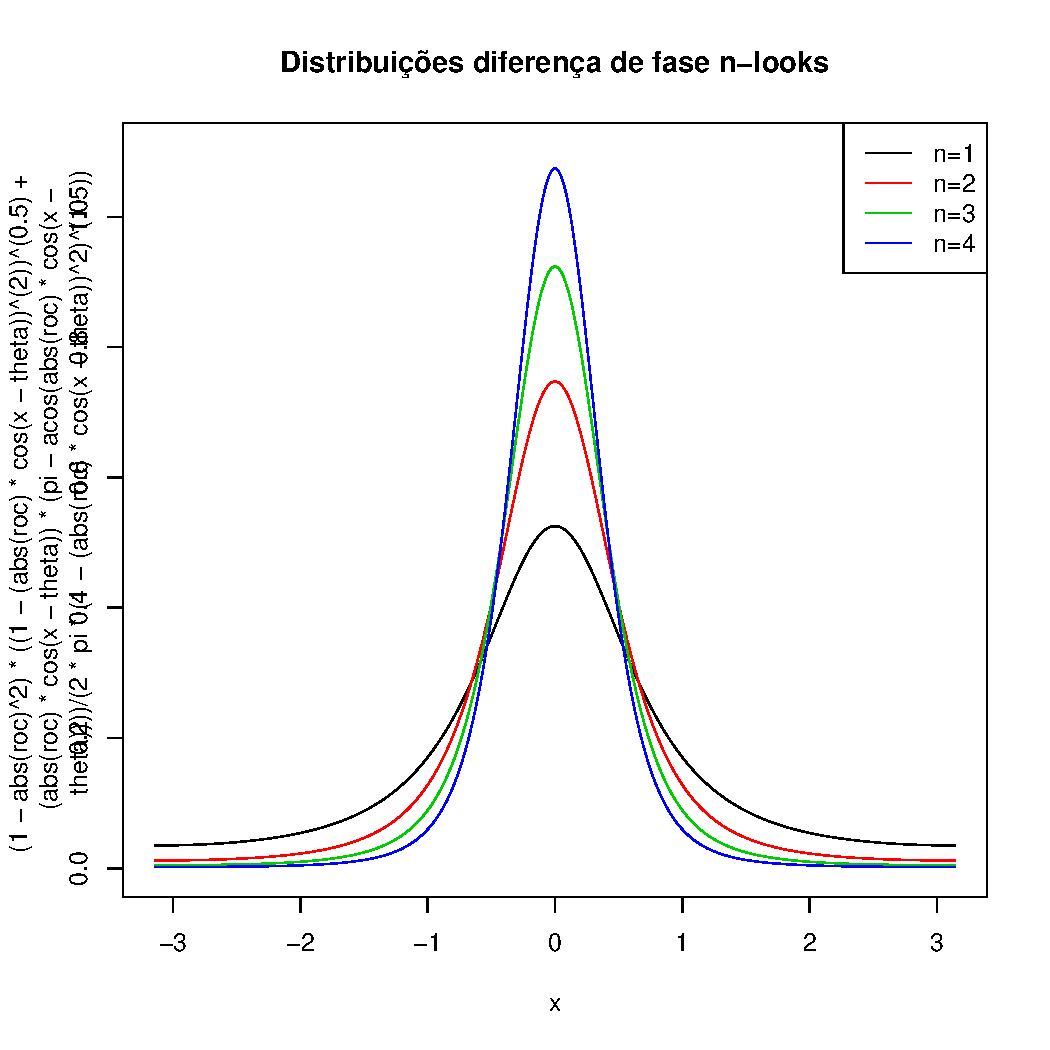
\includegraphics[width=37.0in]{fig1_eq_18_lee_1994.pdf}
	\caption{Distribuição diferença de fase {\it n-looks}.}
\label{fig1}
\end{figure}

A  figura (\ref{fig1}) mostra a equação (\ref{eqn53}) para seus diferentes {\it 1,2,3 e 4 - looks} que são $p_{\psi}^{(1)}(\psi)$, $p_{\psi}^{(2)}(\psi)$, $p_{\psi}^{(3)}(\psi)$ e $p_{\psi}^{(4)}(\psi)$.

\subsubsection{Distribuição conjunta do {\it Multilook} $|S_i|^2$ e $|S_j|^2$ }

O $PDF$ conjunto retorna de dois canais correlacionados dos radares polarimétricos e interferométricos são importantes. As $PDF's$ conjuntas conduzem a derivação da intensidade e amplitude razão $PDF's$. Da equação (\ref{eqn42}) temos que as intensidades {\it multilook} sejam 

\begin{equation}\label{eqn59}
\begin{array}{ccccc}
	R_1&=&\frac{1}{n}\sum_{k=1}^{n}|S_i(k)|^2&=&\frac{B_1C_{11}}{n}\\
	R_2&=&\frac{1}{n}\sum_{k=1}^{n}|S_j(k)|^2&=&\frac{B_2C_{22}}{n}\\
\end{array}
\end{equation}

Integrando a equação (\ref{eqn52}) em relação a $\eta$ e $\psi$. A $PDF$ é

\begin{equation}\label{eqn60}
	p(B_1,B_2)=\frac{\left(B_1B_2\right)^{\frac{n-1}{2}}\exp\left(-\frac{B_1+B_2}{1-|\rho_c|^2}\right)}{\Gamma(n)(1-|\rho_c|^2)|\rho_c|^{n-1}}I_{n-1}\left(2\sqrt{B_1B_2}\frac{|\rho_c|}{1-|\rho_c|^2}\right)
\end{equation}

Sendo
\begin{equation}\label{eqn61}
	I_{\mu}(Z)=\frac{(\frac{z}{2})^{\mu}}{\Gamma(\mu+1)} F_{1}^{0}[-;\mu+1;\frac{z^2}{4}]
\end{equation}

\textcolor{red}{OBS: As integrações na equação (\ref{eqn52}) não foram realizadas neste estudo.}
\begin{equation}\label{eqn62}
	p(B_1,B_2)=\frac{n^{n+1}\left(R_1R_2\right)^{\frac{n-1}{2}}\exp\left(-\frac{n(\frac{R_1}{C_{11}}+\frac{R_2}{C_{22}})}{1-|\rho_c|^2}\right)}{(C_{11}C_{22})^{\frac{n+1}{2}}\Gamma(n)(1-|\rho_c|^2)|\rho_c|^{n-1}}I_{n-1}\left(2n\sqrt{\frac{R_1R_2}{C_{11}C_{22}}}\frac{|\rho_c|}{1-|\rho_c|^2}\right)
\end{equation}

\textcolor{red}{OBS: Verificar o surgimento de um fator $\frac{n^2}{C_{11}C_{22}}$ na equação  (\ref{eqn62}) - Mudança de variável!!!!!.}

\subsubsection{Distribuição razão intensidade e amplitude para {\it multilook}}

A razão de intensidade e amplitude entre $S_{hh}$ e $S_{vv}$ são importantes no estudo de radares polarimétricos. A $PDF's$ razão de intensidade e amplitude normalizada será mostrada agora

\begin{equation}\label{eqn63}
\begin{array}{ccccccc}
	\mu&=&\frac{B_1}{B_2}&=&\frac{\sum_{k=1}^{n}\frac{|S_i(k)|^2}{C_{11}}}{\sum_{k=1}^{n}\frac{|S_j(k)|^2}{C_{22}}}&=&\frac{\sum_{k=1}^{n}|S_i(k)|^2}{\tau\sum_{k=1}^{n}|S_j(k)|^2}\\
\end{array}
\end{equation}

Onde $\tau=\frac{C_{11}}{C_{22}}$.

A $PDF$ razão intensidade {\it multlook} normalizada é mostrada no apêndice $(C)$ do artigo \cite{lee}  


\begin{equation}\label{eqn64}
	p^{(n)}(\mu)=\frac{\Gamma(2n)(1-|\rho_c|^2)^{n}(1+\mu)\mu^{n-1}}{\Gamma(n)\Gamma(n)\left[(1+\mu)^2-4|\rho_c|^2\mu \right]^{\frac{2n+1}{2}}}\\
\end{equation}

\textcolor{red}{OBS: Não realizei as contas do apêndice $(C)$.}

Realizando a troca de variável $\nu=\sqrt{\mu}$ a equação (\ref{eqn64}) pode ser rescrita por
\begin{equation}\label{eqn65}
	p^{(n)}(\nu)=\frac{2\Gamma(2n)(1-|\rho_c|^2)^{n}(1+\nu^2)\nu^{2n-1}}{\Gamma(n)\Gamma(n)\left[(1+\nu^2)^2-4|\rho_c|^2\nu^2 \right]^{\frac{2n+1}{2}}}\\
\end{equation}
As $PDF's$ razão de intensidade e amplitude entre os {\it multilook} $\mathbf{S_1}$ e $\mathbf{S_2}$ podem ser facilmente deduzidas das seguintes definições e posterior aplicação nas equações (\ref{eqn64}) e (\ref{eqn65}). definindo 
\begin{equation}\label{eqn66}
\begin{array}{ccccc}
	w&=&\frac{\sum_{k=1}^{n}|S_i(k)|^2}{\sum_{k=1}^{n}|S_i(k)|^2}&=&\tau\mu\\
	z&=&\sqrt{w}&=&\sqrt{\tau}\nu
\end{array}
\end{equation}
Portanto a distribuição da razão $w$ de intensidade {\it multilook} é
\begin{equation}\label{eqn67}
	p^{(n)}(w)=\frac{\tau^{n}\Gamma(2n)(1-|\rho_c|^2)^{n}(\tau+w)w^{n-1}}{\Gamma(n)\Gamma(n)\left[(\tau+w)^2-4\tau|\rho_c|^2w \right]^{\frac{2n+1}{2}}}.
\end{equation}
Portanto a distribuição da razão $z$ de amplitude {\it multilook} é
\begin{equation}\label{eqn68}
	p^{(n)}(z)=\frac{\tau^{n}\Gamma(2n)(1-|\rho_c|^2)^{n}(\tau+z^2)z^{2n-1}}{\Gamma(n)\Gamma(n)\left[(\tau+z^2)^2-4\tau|\rho_c|^2z^2 \right]^{\frac{2n+1}{2}}}.
\end{equation}

A discusão será limitada para estatística da razão $\nu$ amplitude normalizada. A figura (\ref{fig2}) mostra a distribuição razão amplitude apresentada na equação  (\ref{eqn65}). Notadamente a medida que $n$ aumenta tendemos a ter uma aproximação da "função" delta de Dirac e uma concentração em torno da abscissa $\nu=1$.

\textcolor{blue}{OBS: Processos de {\it multilook} reduzem a variância.}

\begin{figure}[hbt]
\centering
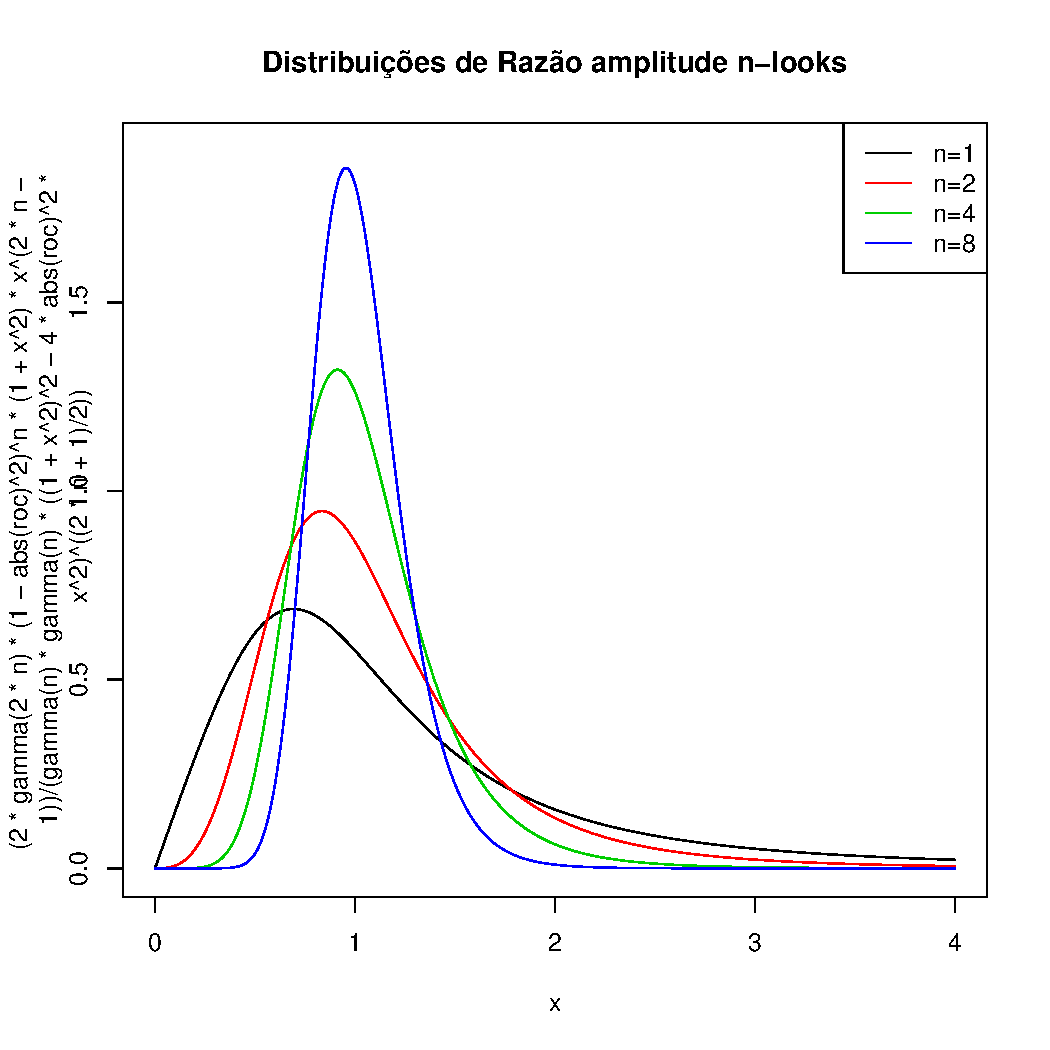
\includegraphics[width=4.0in]{fig4_eq_33_lee_1994.pdf}
	\caption{Distribuição de razão amplitude {\it n-looks}.}
\label{fig2}
\end{figure}


\subsection{Estudo do artigo  \cite{good}}


A variável randômica gaussiana complexa $\mathbf{Z=X+iY}$ é uma variável randômica complexa cuja parte imaginária e complexa são distribuída de forma Gaussiana.  E uma variável randômica gaussiana complexa $p-$variada $\xi^{'}=(Z_1,Z_2,\dots,Z_p)$ é uma $p-$upla  de variáveis randômica gaussiana complexas tal que o vetor de partes imaginárias e reais é $\eta^{'}=(X_1,Y_1,\dots,X_p,Y_p)$.

A matriz de covariância definida positiva $2p\times 2p$ será:
$$
\mathbf{\Sigma_{\eta}} = \left[
\begin{array}{cc}
	E(X_jX_k)  & E(X_jY_k)  \\
	E(Y_jX_k)  & E(Y_jY_k)  \\
\end{array}
\right].
$$
Tal que
$$
\mathbf{\Sigma_{\eta}} = \left[
\begin{array}{cc}
	E(X_jX_k)  & E(X_jY_k)  \\
	E(Y_jX_k)  & E(Y_jY_k)  \\
\end{array}
\right]= \left\{
\begin{array}{cc}
	\frac{1}{2}\left[
\begin{array}{cc}
	 1 & 0  \\
	 0 & 1  \\
\end{array}
	\right]\sigma^{2}_{k}  & \mbox{se}\quad j=k, \\
	& \\
	\frac{1}{2}\left[
\begin{array}{cc}
	\alpha_{ik} & -\beta_{jk}  \\
	 \beta_{jk} & \alpha_{ik}  \\
\end{array}
	\right]\sigma_j\sigma_k  & \mbox{se}\quad j\neq k.   \\
\end{array}
\right.
$$

Onde $E(\cdot)$ denota o operador de valor esperado(esperança).

Podemos usar a matriz de covariância hermitiana complexa definida positiva usando a $\xi$ variável randômica gaussiana complexa de dimensão $p\times p$

$$\Sigma_{\xi}=E(\xi\bar{\xi}^{T})=||E(Z_j\bar{Z}_k)||=||\sigma_{jk}||$$

onde

$$
\sigma_{jk} = \left\{
\begin{array}{cc}
	\sigma_k^2                                & \mbox{se}\quad j=k,  \\
	(\alpha_{jk}+i\beta_{jk})\sigma_j\sigma_k & \mbox{se}\quad j\neq k. \\
\end{array}
\right.
$$

A função densidade de probabilidade ({\bf pdf}) da distribuição gaussiana complexa $p-$variada é dada por
\begin{equation}\label{eqn69}
	p(\xi)=\frac{1}{\pi^p|\Sigma_{\xi}|}\exp(-\bar{\xi}^{T}\Sigma_{\xi}^{-1}\xi)  \\
\end{equation}


{\bf Exemplo 1 -} Seja a distribuição gaussian complexa univariada $(p=1)$. Sendo $\xi^{T}=z_1=x_1+iy_1$. E a "matriz" de covariância $\Sigma_{\xi}=\sigma_{1}^{2}$ com determinante $|\Sigma_{\xi}|=\sigma_{1}^{2}$ e  "matriz inversa" $\Sigma_{\xi}^{-1}=\frac{1}{\sigma_{1}^{2}}$, Assim,

\begin{equation}\label{eqn70}
\begin{array}{ccc}
	\bar{\xi}^{T}\Sigma_{\xi}^{-1}\xi&=&(x_i-iy_1)\frac{1}{\sigma_1^2}(x_1+iy_1)  \\
	\bar{\xi}^{T}\Sigma_{\xi}^{-1}\xi&=&(x_i-iy_1)(x_1+iy_1)\frac{1}{\sigma_1^2}  \\
	\bar{\xi}^{T}\Sigma_{\xi}^{-1}\xi&=&\frac{x_1^2+y_1^2}{\sigma_1^2}  \\
\end{array}
\end{equation}


\begin{equation}\label{eqn71}
	p(\xi)=\frac{1}{\pi\Sigma_{\xi}^{2}}\exp\left(-\frac{x_1^2+y_1^2}{\sigma_1^2}\right)  \\
\end{equation}

{\bf Exemplo 2 -} Seja a distribuição gaussian complexa bivariada $(p=2)$. Sendo $\xi^{T}=(z_1, z_2)=(x_1 + iy_1, x_2 + iy_2)^{T}$. E a matriz de covariância 

$$
\Sigma_{\xi} = \left[
\begin{array}{cc}
	\sigma_1^2                                &  (\alpha_{12}+i\beta_{12})\sigma_1\sigma_2  \\
	(\alpha_{12}-i\beta_{12})\sigma_j\sigma_k & \sigma_2^2 \\
\end{array}
\right].
$$
com determinante $|\Sigma_{\xi}|=(1 - \sigma_{12}^{2}- \beta_{12}^2)\sigma_{1}^2\sigma_{2}^2$ e  matriz inversa 
$$
\Sigma_{\xi}^{-1} =\frac{1}{(1 - \sigma_{12}^{2}- \beta_{12}^2)\sigma_{1}^2\sigma_{2}^2} \left[
\begin{array}{cc}
	\sigma_2^2                                &  -(\alpha_{12}+i\beta_{12})\sigma_1\sigma_2  \\
	-(\alpha_{12}-i\beta_{12})\sigma_j\sigma_k & \sigma_1^2 \\
\end{array}
\right].
$$
\begin{equation}\label{eqn72}
\begin{array}{ccc}
	\bar{\xi}^{T}\Sigma_{\xi}^{-1}\xi&=&[z_1,z_2]^{H}\Sigma_{\xi}^{-1}
	\left[
\begin{array}{c}
	z_1  \\
	z_2 \\
\end{array}\right]\\
\end{array}
\end{equation}
\begin{equation}\label{eqn73}
\begin{array}{ccc}
	\bar{\xi}^{T}\Sigma_{\xi}^{-1}\xi&=&[z_1,z_2]^{H}\frac{1}{(1 - \sigma_{12}^{2}- \beta_{12}^2)\sigma_{1}^2\sigma_{2}^2} \left[
\begin{array}{cc}
	\sigma_2^2                                &  -(\alpha_{12}+i\beta_{12})\sigma_1\sigma_2  \\
	-(\alpha_{12}-i\beta_{12})\sigma_1\sigma_2 & \sigma_1^2 \\
\end{array}
\right]
	\left[
\begin{array}{c}
	z_1  \\
	z_2 \\
\end{array}\right]\\
\end{array}
\end{equation}

\begin{equation}\label{eqn74}
\begin{array}{ccc}
	\bar{\xi}^{T}\Sigma_{\xi}^{-1}\xi&=&\frac{1}{(1 - \sigma_{12}^{2}- \beta_{12}^2)\sigma_{1}^2\sigma_{2}^2} [z_1,z_2]^{H}\left[
\begin{array}{cc}
	\sigma_2^2                                &  -(\alpha_{12}+i\beta_{12})\sigma_1\sigma_2  \\
	-(\alpha_{12}-i\beta_{12})\sigma_1\sigma_2 & \sigma_1^2 \\
\end{array}
\right]
	\left[
\begin{array}{c}
	z_1  \\
	z_2 \\
\end{array}\right]\\
\end{array}
\end{equation}

\begin{equation}\label{eqn75}
\begin{array}{ccc}
	\bar{\xi}^{T}\Sigma_{\xi}^{-1}\xi&=&\frac{1}{(1 - \sigma_{12}^{2}- \beta_{12}^2)\sigma_{1}^2\sigma_{2}^2} [z_1,z_2]^{H}\left[
\begin{array}{cc}
	\sigma_2^2z_1-(\alpha_{12}+i\beta_{12})\sigma_1\sigma_2z_2  \\
	-(\alpha_{12}-i\beta_{12})\sigma_1\sigma_2z_1+\sigma_1^2z_2 \\
\end{array}
\right]
\end{array}
\end{equation}

\begin{equation}\label{eqn76}
	\bar{\xi}^{T}\Sigma_{\xi}^{-1}\xi=\frac{1}{(1 - \sigma_{12}^{2}- \beta_{12}^2)\sigma_{1}^2\sigma_{2}^2}\left(
	\sigma_2^2\bar{z_1}z_1-(\alpha_{12}+i\beta_{12})\sigma_1\sigma_2\bar{z_1}z_2 
	-(\alpha_{12}-i\beta_{12})\sigma_1\sigma_2\bar{z_2}z_1+\sigma_1^2\bar{z_2}z_2 \right)
\end{equation}

\begin{equation}\label{eqn77}
	\bar{\xi}^{T}\Sigma_{\xi}^{-1}\xi=\frac{1}{(1 - \sigma_{12}^{2}- \beta_{12}^2)\sigma_{1}^2\sigma_{2}^2}\left(
	\sigma_2^2|z_1|^2+\sigma_1^2|z_2|^2-2\alpha_{12}\sigma_1\sigma_2\bar{z_1}z_2 	\right)
\end{equation}

\begin{equation}\label{eqn78}
	\bar{\xi}^{T}\Sigma_{\xi}^{-1}\xi=\frac{\sigma_2^2|z_1|^2+\sigma_1^2|z_2|^2-2\alpha_{12}\sigma_1\sigma_2\bar{z_1}z_2}{(1 - \sigma_{12}^{2}- \beta_{12}^2)\sigma_{1}^2\sigma_{2}^2}
\end{equation}

Assim, a função densidade de probabilidade ({\bf pdf}) 

\begin{equation}\label{eqn79}
	p(\xi)=\frac{1}{\pi^2(1 - \sigma_{12}^{2}- \beta_{12}^2)\sigma_{1}^2\sigma_{2}^2}\exp\left(-\frac{\sigma_2^2|z_1|^2+\sigma_1^2|z_2|^2-2\alpha_{12}\sigma_1\sigma_2\bar{z_1}z_2}{(1 - \sigma_{12}^{2}- \beta_{12}^2)\sigma_{1}^2\sigma_{2}^2}
\right)  
\end{equation}

{\bf Distribuição complexa de Wishart}

A distribuição complexa de Wishart descrita no artigo \cite{good}, define agora uma amostra de  $n$ vetores com valores complexos $\xi_1,\xi_2,\dots,\xi_n$ então a matriz hermitiana de covariância é 

\begin{equation}\label{eqn80}
	\hat{\Sigma}_{\xi}=\frac{1}{n}\sum_{j=1}^{n}\xi_j\bar{\xi}_{j}^{T} . \\
\end{equation}

A matriz $\hat{\Sigma}_{\xi}$ é uma "maximum likelihood" para $\Sigma_{\xi}$ sendo uma estatística suficiente para a matriz hermitiana de covariância.

Considerando $A=||A_{jkR}+iA{jkI}||=n\hat{\Sigma}_{\xi}$ chamaremos a matriz $A$ de distribuição complexa de Wishart. A função densidade de probabilidade de $A$ é
\begin{equation}\label{eqn81}
	p_W(A)=\frac{|A|^{n-p}}{I(\Sigma_{\xi})} \exp(-tr(\Sigma_{\xi}^{-1}A)), 
\end{equation}
onde
\begin{equation}\label{eqn82}
	I(\Sigma_{\xi})=\pi^{\frac{1}{2}p(p-1)}\Gamma(n)\cdots\Gamma(n-p+1)|\Sigma_{\xi}|^n, 
\end{equation}
sendo $\Gamma(\cdot)$ a função Gamma.

\subsection{Estudo do artigo  \cite{smp}}

Definição importante  

\begin{definition}{Divergência ($h,\phi$).}
	Sejam as variáveis aleatórias $X$ e $Y$ com mesmo suporte $S$  e $p.d.f$ respectivamente $f_{X}(x|\theta_1)$ e $f_{Y}(x|\theta_2)$. Sejam ainda $\phi:(0,\infty)\rightarrow \mathbb{R}_+$ uma função convexa e diferenciável, e $h$ uma função crescente tal que $h(0)=0$ então a divergência ($h,\phi$) é definida como
\begin{equation}\label{eqn83}
	d_{\phi}^{h}(X||Y)=h\left[\int_{x\in S(x)} f_{Y}(x|\theta_2)\phi\left(\frac{f_{X}(x|\theta_1)}{f_{Y}(x|\theta_2)}\right)dx \right]. \\
\end{equation}
\end{definition}

Definindo que divergência é uma maneira de medir as diferenças entre duas distribuições. A seguir descreveremos um exemplo para ilustrar a definição.

Para começar a entender os resultados do artigo \cite{smp} é descrito abaixo o exemplo 1 sobre medida craniana de rãs:

Sendo $(x_1)$ o comprimento craniano e $(x_2)$ a amplitude craniana, uma amostra de $n=35$ rãs femeas maduras conduziu a seguinte estatística:

$$
\mathbf{x_1} = \left[
\begin{array}{c}
	22.860   \\
	24.397   \\
\end{array}
\right]
\mathbf{S_1} = \left[
\begin{array}{cc}
	 17.178  & 19.710   \\
         19.710  & 23.710   \\
\end{array}
\right].
$$

e similar medidas para uma amostra $m=14$ rãs machos, 

$$
\mathbf{x_2} = \left[
\begin{array}{c}
	21.821  \\
	22.843   \\
\end{array}
\right]
\mathbf{S_2} = \left[
\begin{array}{cc}
	 17.159  & 17.731   \\
         17.731  & 19.273   \\
\end{array}
\right].
$$

onde $\mathbf{S_1}$ e $\mathbf{S_2}$ são estimadores de máxima varossimilhança da matriz de covariância.

Para auxiliar foi criado dois programas em matlab chamados "salicruex1a.m" e "salicru1ex1b.m" armazenado em (meu micro): $$"/home/aborba/MEGAsync/mack/alejandro/gitufalmackbackup/doclatex/"$$


\begin{description}
\item[(a)] Sendo:
$$
		\mathbf{S}=\frac{n\mathbf{S_1}+m\mathbf{S_2}}{n+m} = \left[
\begin{array}{cc}
	 17.173  & 19.145   \\
         19.145  & 22.442   \\
\end{array}
\right].
$$
tal que sua matriz inversa é:
$$
		\mathbf{S^{-1}} = \left[
\begin{array}{cc}
	 1.18958  & -1.01482   \\
        -1.01482  & 0.91028   \\
\end{array}
\right].
$$

		A expressão $(r,s)$-divergência obtida de $(h,\phi)$-divergência sobre certas condições pode ser escrita:
\begin{equation}\label{eqn84}
\begin{array}{ccl}
	D_r^s((\mu_1,\Sigma_1),(\mu_2,\Sigma_2))&=&\frac{1}{(s-1)}\left[\exp\left(\frac{r(s-1)}{2}(\mu_1-\mu_2)^{T}[r\Sigma_2+(1-r)\Sigma_1]^{-1}(\mu_1-\mu_2) \right)\right. \\
	&\cdot&\left.\frac{|r\Sigma_2+(1-r)\Sigma_1|^{\frac{(1-s)}{2(r-1)}}}{|\Sigma_1|^{\frac{s-1}{2}}|\Sigma_2|^{\frac{(1-s)r}{2(r-1)}}}-1\right]  \\
\end{array}
\end{equation}

Assim calculando
\begin{equation}\label{eqn85}
\begin{array}{ccc}
	T_4&=&\frac{2nm}{r(n+m)}D_r^s((\mathbf{x_1}, \mathbf{S}),(\mathbf{x_2}, \mathbf{S})) \\
	T_4&=&40(0.052663) \\
	T_4&=&2.10653
\end{array}
\end{equation}
\item[(b)] Será usado o corolário $2b$ do artigo \cite{smp} assim a estatística que vamos calcular será:

\begin{equation}\label{eqn86}
\begin{array}{ccc}
	T_3&=&\frac{2nm}{r(n+m)}D_r^s((\mathbf{x_1}, \mathbf{S_1}),(\mathbf{x_2}, \mathbf{S_2})) \\
	T_3&=&4.76047
\end{array}
\end{equation}

Tendo um valor diferente do artigo, investigando onde pode estar a discrepância encontramos o seguinte valor para, 

\begin{equation}\label{eqn87}
	(\mathbf{x_1}-\mathbf{x_2})^T [r\mathbf{S_2+(1-r)S_1}]^{-1}(\mathbf{x_1-x_2})= 0.22724\\
\end{equation}

enquanto o artigo encontrou $0.06970$ para o mesmo passo, até o momento não sei explicar a diferença.

\end{description}


\subsection{Estudo do artigo  \cite{ade}}

O instrumento SAR totalmente polarimétrico transmite pulsos de microondas polarizados ortogonalmente e mede componentes ortogonais do sinal recebido. Para cada pixel a medida resulta em uma matriz de coeficientes de espalhamento. Esses coeficientes são números complexos que descrevem a transformação do campo eletromagnético trasmitido para o campo eletromagnético recebido para todas as combinações de transmitidas e recebidas polarizações.

A transformação pode ser representada como

\begin{equation}\label{eqn88}
 \left[
\begin{array}{c}
	E_{h}^{r}   \\
	E_{v}^{r}    \\
\end{array}
\right]
 = \frac{e^{jkr}}{r}\left[
\begin{array}{cc}
	S_{hh}   & S_{hv}   \\
	S_{vh}   & S_{vv}   \\
\end{array}
\right]
 \left[
\begin{array}{c}
	E_{h}^{t}   \\
	E_{v}^{t}    \\
\end{array}
\right]
\end{equation}

Onde $k$ denota o número de onda e $r$ é a distância entre o radar e o alvo. No campo eletromagnético com componentes $E_{i}^{j}$ os índices subscritos denotados polarização horizontal $h$ ou vertical $v$ enquanto os índices sobrescritos indicam a onda recebida $r$ ou transmitida $t$.    


A matrix de espalhamento pode ser reduzida ao seguintes vetores:

\begin{equation}\label{eqn89}
\mathbf{s} = \left[
\begin{array}{c}
	S_{hh}      \\
	\frac{S_{hv}+S_{vh}}{\sqrt{2}}     \\
	S_{vv}      \\
\end{array}
\right],
\mathbf{k} =\frac{1}{\sqrt{2}} \left[
\begin{array}{c}
	S_{hh} + S_{vv}      \\
	S_{hh} - S_{vv}      \\
	S_{hv} + S_{vh}      \\
\end{array}
\right].
\end{equation}

%De acordo com \cite{goodman1963} a distribuíção gaussiana complexa multivariada pode modelar adequadamente o comportamento estatístico de $\mathbf{ S$. Isto é chamado de {\it single-look PolSar data representation} e podemos definir o vetor de espalhamento por ${\mathbf s}=[S_1,S_2,\dots,S_p]^T$. 

%A função densidade de probabilidade ({\bf pdf}) da distribuição gaussiana complexa $p-$variada é dada por
%\begin{equation}\label{sec1eqn2}
%\begin{array}{ccc}
%	p({\bf s})&=&\frac{1}{\pi^p|\Sigma_{{\bf s}}|}\exp(-\bar{{\bf s}}^{T}\Sigma_{{\bf s}}^{-1}{\bf s})  \\
%\end{array}
%\end{equation}

%Sendo a matriz de covariância definida por:
%\begin{equation}\label{sec1eqn2}
%	{\bf \Sigma_{{\bf s}}} = E[{\bf s}{\bf s}^H] \left[
%\begin{array}{cccc}
%	E({\bf s_1}{\bf s_1}^H)  & E({\bf s_1}{\bf s_2}^H) &\hdots & E({\bf s_1}{\bf s_p}^H) \\
%	E({\bf s_2}{\bf s_1}^H)  & E({\bf s_2}{\bf s_2}^H) &\hdots &E({\bf s_2}{\bf s_p}^H)\\
%        \vdots&\vdots &\ddots &\vdots\\
%	E({\bf s_p}{\bf s_1}^H)  & E({\bf s_p}{\bf s_2}^H) &\hdots &E({\bf s_p}{\bf s_p}^H)\\
%\end{array}
%\right].
%\end{equation}

%onde $E(\cdot)$ e $(\cdot)^H$ denotam o valor esperado e o conjugado transposto.

%Dados polarimétricos são usualmente sujeitados a um processo {\it multilook} com o intuito de melhorar a razão {\it signal-to-noise}. Para esse fim, matrizes positivas definidas hermitianas são obtidas computando a médias de $L$ {\it looks} independentes de uma mesma cena. Isto resulta na matriz de covariância {\bf Z} dada por:

%\begin{equation}\label{sec1eqn3}
%\begin{array}{ccc}
%	{\bf Z}&=&\frac{1}{n}\displaystyle{\sum_{i=1}^{L} {\bf s_i}{\bf s_i}^H} . \\
%\end{array}
%\end{equation}

\subsubsection{Modelos Gaussianos}


Podemos assumir que o vetor de espalhamento é uma distribuíção gaussiana complexa circular. A matriz {\boldmath S} e os vetores {\boldmath s} e {\boldmath k} são {\it Single-look complex} representação dos daos PolSAR. Dados PolSAR {\it Multilook} podem ser representados por
 
\begin{equation}\label{eqn90}
	\mathbf{C_{\mathbf s}}=\frac{1}{L}\sum_{i=1}^{L} \mathbf{s_i s_i}^H ,
	\mathbf{C_{\mathbf k}}=\frac{1}{L}\sum_{i=1}^{L} \mathbf{k_i k_i}^H . \\
\end{equation}

chamadas de matriz de covariância e matriz de coerência, sendo $L$ o número de {\it looks}. Por definição assumimos que {\boldmath s} ou {\boldmath k} é gaussiana multivariada e complexa circular e tem média zero. Será denotado $s\sim N_d^\mathbb{C}(\mathbf{0, \Sigma_{s}})$ onde $\mathbf{0}$ é um vetor coluna de zeros, $d$ a dimensão de $\mathbf{s}$ a matriz de covariância de $\mathbf{s}$  

\begin{equation}\label{eqn91}
	\mathbf{\Sigma_{\mathbf{s}}} = E[\mathbf{s}\mathbf{s}^H] =\left[
\begin{array}{cccc}
	E(\mathbf{s_1s_1}^H)  & E(\mathbf{s_1s_2}^H) &\hdots & E(\mathbf {s_1s_p}^H) \\
	E(\mathbf{s_2 s_1}^H)  & E(\mathbf{ s_2 s_2}^H) &\hdots &E(\mathbf{s_2 s_p}^H)\\
        \vdots&\vdots &\ddots &\vdots\\
	E(\mathbf{s_p s_1}^H)  & E(\mathbf{s_ps_2}^H) &\hdots &E(\mathbf{s_p s_p}^H)\\
\end{array}
\right].
\end{equation}

A função densidade de probabilidade $(pdf)$ de {\boldmath s} é 

\begin{equation}\label{eqn92}
	p(\mathbf{s},\Sigma_{\mathbf{s}})=\frac{1}{\pi^p|\Sigma_{\mathbf{s}}|}\exp(-\mathbf{s}^{H}\Sigma_{\mathbf{s}}^{-1}\mathbf{s})  \\
\end{equation}

Se $L\geq d$ e os {\boldmath$S_i$} (ou {\boldmath$k_i$}) e na equação (\ref{eqn90}) são independentes, então ma matriz de covariância escalada pode ser definida como $\mathbf{Z}=L\mathbf{C_{\mathbf s}}$ (ou $\mathbf{Z}=L\mathbf{C_k}$), de acordo com distribuição de Wishart complexa não singular \cite{good}

\begin{equation}\label{eqn93}
	p_{\mathbf{Z}}(\mathbf{Z};L,\mathbf{\Sigma})=\frac{|\mathbf{Z}|^{L-p}}{|\mathbf{\Sigma}|^{L}\Gamma_d(L)} \exp(-tr(\mathbf{\Sigma}^{-1}\mathbf{Z})), \\
\end{equation}
onde $tr(\cdot)$ é o operador traço e ${\Sigma}=\frac{E[\mathbf{Z}]}{L}=E[\mathbf{C_{s}}]$. 

Vamos escrever $\mathbf{Z}\sim W_d^{\mathbb C}(L, \mathbf{\Sigma})$.

E ainda, A constante de normalização $\Gamma_d(L)$ é a função Gamma multivariada definida como 
\begin{equation}\label{eqn94}
	\Gamma_d(L)=\pi^{\frac{1}{2}d(d-1)} \prod_{i=0}^{d-1}\Gamma(L-i) \\
\end{equation}
sendo $\Gamma(\cdot)$ a função Gamma.

Seja a distribuição complexa Wishart (\ref{eqn93}) vamos encontrar a derivada do logaritmo natural desta distribuição em relação ao número de {\it looks}.
\begin{equation}\label{eqn95}
\begin{array}{ccc}
	\ln{p_{\mathbf{Z}}(\mathbf{Z};L,\mathbf{\Sigma})}&=&\ln{\left(\frac{|\mathbf{Z}|^{L-p}}{|\mathbf{\Sigma}|^{L}\Gamma_d(L)} \exp(-tr(\mathbf{\Sigma}^{-1}\mathbf{Z}))\right)}, \\
	\ln{\left(p_{\mathbf{Z}}(\mathbf{Z};L,\mathbf{\Sigma})\right)}&=&\ln{\left(\frac{|\mathbf{Z}|^{L-p}}{|\mathbf{\Sigma}|^{L}\Gamma_d(L)}\right)}+\ln{\left( \exp(-tr(\mathbf{\Sigma}^{-1}\mathbf{Z}))\right)}, \\
	\ln{\left(p_{\mathbf{Z}}(\mathbf{Z};L,\mathbf{\Sigma})\right)}&=&\ln{\left(|\mathbf{Z}|^{L-p}\right)} - \ln{\left(|\mathbf{\Sigma}|^{L}\Gamma_d(L)\right)}-tr(\mathbf{\Sigma}^{-1}\mathbf{Z}), \\
	\ln{\left(p_{\mathbf{Z}}(\mathbf{Z};L,\mathbf{\Sigma})\right)}&=&(L-p)\ln{\left(|\mathbf{Z}|\right)} - \ln{\left(|\mathbf{\Sigma}|^{L}\right)}-\ln{\left(\Gamma_d(L)\right)}-tr(\mathbf{\Sigma}^{-1}\mathbf {Z}), \\
	\ln{\left(p_{\mathbf{Z}}(\mathbf{Z};L,\mathbf{\Sigma})\right)}&=&L\ln{\left(|\mathbf{Z}|\right)}-p\ln{\left(|\mathbf{Z}|\right)} - L\ln{\left(|\mathbf{\Sigma}|\right)}-\ln{\left(\Gamma_d(L)\right)}-tr(\mathbf{\Sigma}^{-1}\mathbf{Z}). \\
\end{array}
\end{equation}
% % % ACF Só coloque parênteses necessários, veja a primeira equação

Derivando o logaritmo da densidade em relação a $L$ teremos:
\begin{equation}\label{eqn96}
\begin{array}{ccc}
	\frac{\partial}{\partial L}\left(\ln{\left(p_{\mathbf{Z}}(\mathbf{Z};L,\mathbf{\Sigma})\right)}\right)&=&\frac{\partial}{\partial L}\left(L\ln{\left(|\mathbf{Z}|\right)}-p\ln{\left(|\mathbf{Z}|\right)} - L\ln{\left(|\mathbf{\Sigma}|\right)}-\ln{\left(\Gamma_d(L)\right)}-tr(\mathbf{\Sigma}^{-1}\mathbf{Z})\right). \\
	\frac{\partial}{\partial L}\left(\ln{\left(p_{\mathbf{Z}}(\mathbf{Z};L,\mathbf{\Sigma})\right)}\right)&=&\ln{\left(|\mathbf{Z}|\right)} - \ln{\left(|\mathbf{\Sigma}|\right)}-\frac{\partial}{\partial L}\left(\ln{\left(\Gamma_d(L)\right)}\right). \\
	\frac{\partial}{\partial L}\left(\ln{\left(p_{\mathbf{Z}}(\mathbf{Z};L,\mathbf{\Sigma})\right)}\right)&=&\ln{\left(\frac{|\mathbf{Z}|}{|\mathbf{\Sigma}|}\right)} - \frac{\Gamma^{'}_d(L)}{\Gamma_d(L)}. \\
\end{array}
\end{equation}
% % % ACF Não coloque uma linha adicional quando é o mesmo parágrafo
isto é, 
% % % ACF
\begin{equation}\label{eqn97}
	\frac{\partial}{\partial L}\left(\ln{\left(p_{\mathbf{Z}}(\mathbf{Z};L,\mathbf{\Sigma})\right)}\right)=\ln{\left(\frac{|\mathbf{Z}|}{|\mathbf{\Sigma}|}\right)} - \frac{\Gamma^{'}_d(L)}{\Gamma_d(L)}. \\
\end{equation}
\subsubsection{Coeficiente de estimador de variação}

O exemplo da figura (\ref{fig3}) mostra uma distribuíção gamma $g(\sigma, L)$ parametrizada com intensidade média $\sigma=0.0358$ e com múmeros de {\it looks} $L=\{8,10,12\}$.
\begin{equation}\label{eqn98}
	p_{I}(I;\sigma,L)=\frac{1}{\Gamma(L)}\left(\frac{L}{\sigma}\right)^L \exp(-\frac{LI}{\sigma}), 
\end{equation}
onde intensidade média $\sigma$ e número de {\it looks} $L$ são parametros desta distribuição gamma.

{\bf obs 1} - Programa {\it proanfinsen2009.r} armazenado no meu computador pessoal.

\begin{figure}[hbt]
\centering
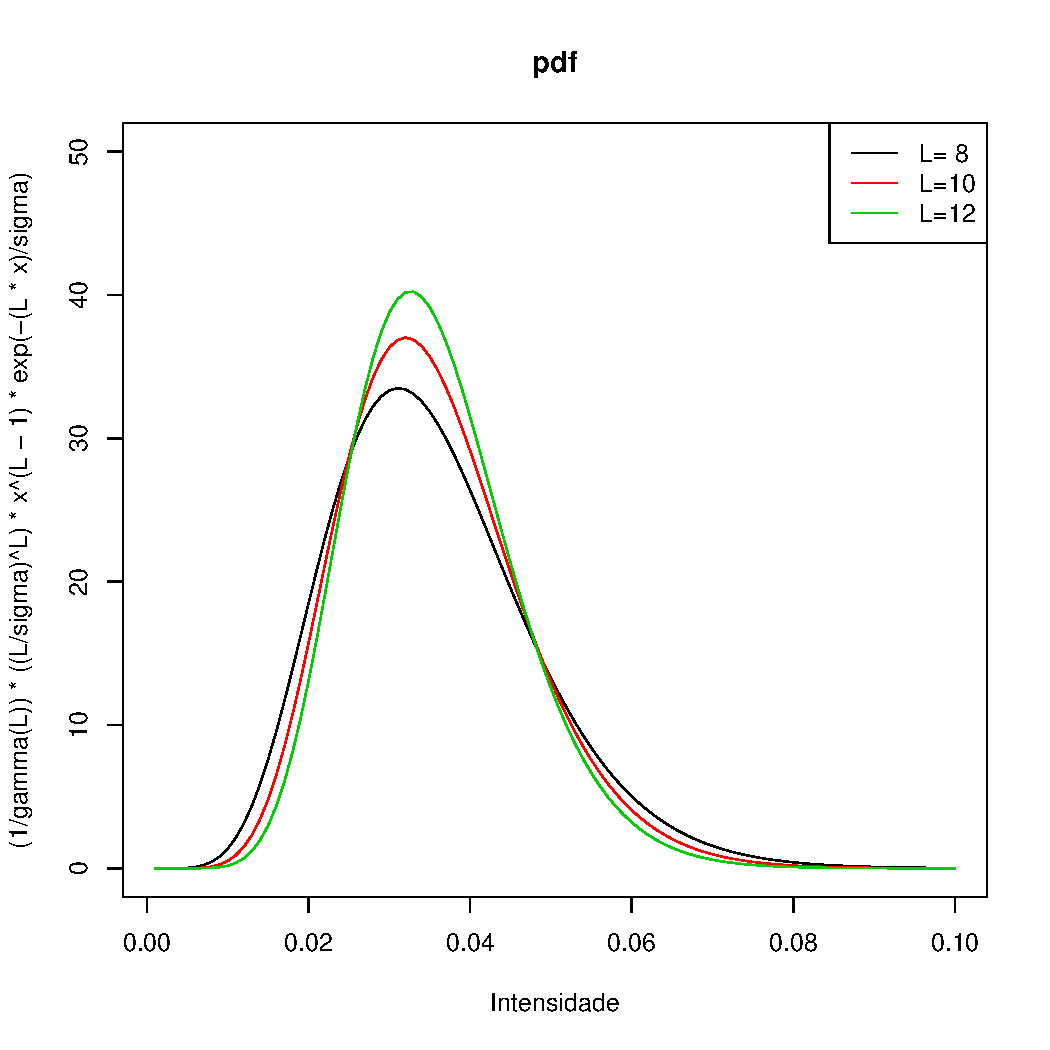
\includegraphics[width=4.0in]{fig_1_anfinsen_2009.pdf}
	\caption{Distribuição gamma da referência \cite{ade} com parametros $\sigma=0.0356$ e $L=\{8,10,12\}$.}
\label{fig3}
\end{figure}

\subsection{Estudo do artigo  \cite{ffc}}

As definições deste artigo são semelhantes as definições do artigo \cite{ade} descrita na seção acima. 

\subsubsection{ Entendendo as densidades e seus gráficos}

Nesta seção o intuito é reproduzir e entender as distribuições que geraram as figuras (1), (2) e (3) do artigo \cite{ffc}. 

\begin{equation}\label{eqn99}
	f_{X}(x)=\frac{r_{\alpha,\omega}}{2K_{\alpha}(\omega)}x^{\alpha-1}\exp\left(-\frac{\omega}{2}\left(\frac{1}{r_{\alpha,\omega}x}+ r_{\alpha,\omega}x\right)\right), \\
\end{equation}

onde $x>0$  e $r_{\alpha,\omega}=\frac{K_{\alpha+1}(\omega)}{K_{\alpha}(\omega)}$

Seja $K_{\nu}$ uma função de Bessel de terceiro tipo e com ordem $\nu$. Na figura (\ref{fig4}) é mostrado os gráficos das funções para diferentes valores de $\nu=1,2,3,4,5,10$ e $\nu=20$. 
\begin{figure}[!htb]
\centering
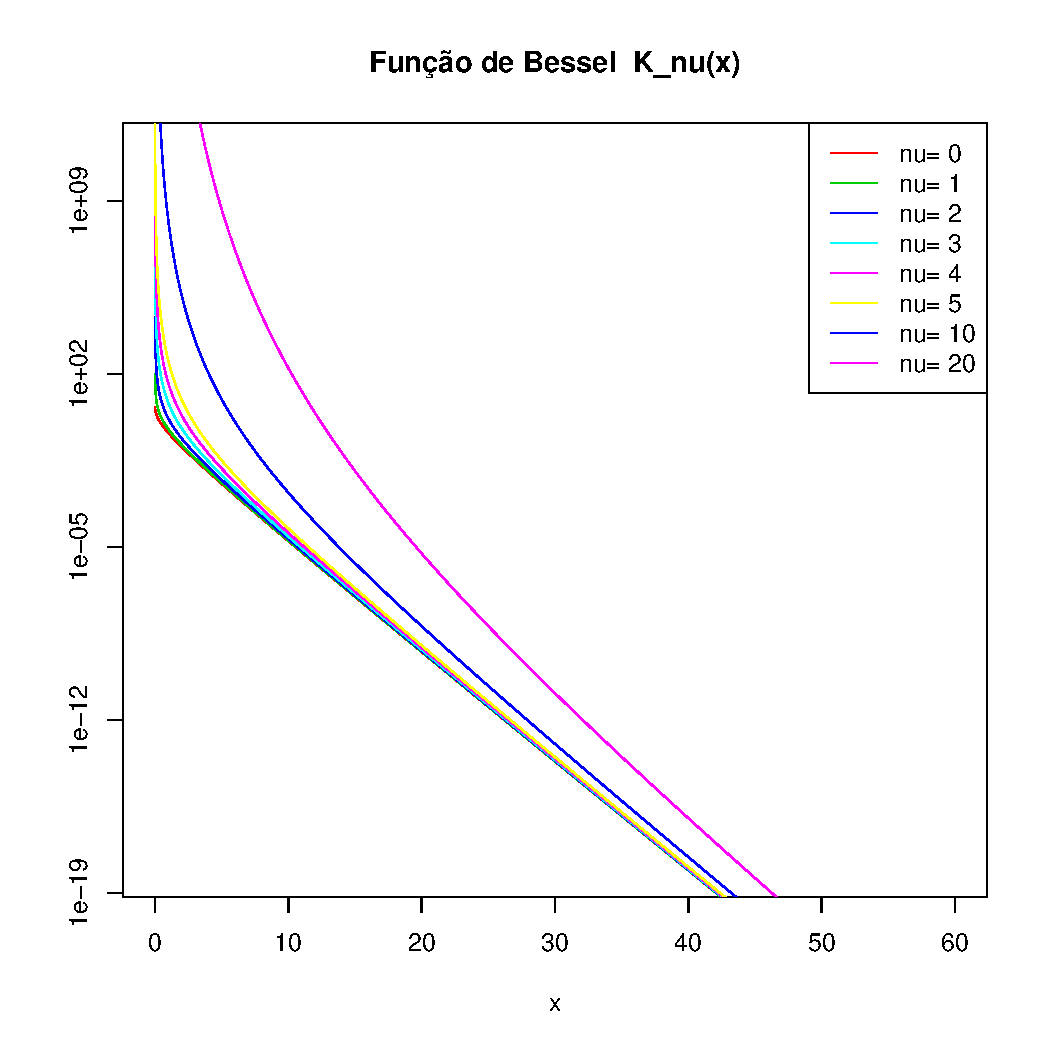
\includegraphics[width=4.0in]{fun_bessel_nu.pdf}
	\caption{Gráficos da referência \cite{ffc} para as funções de Bessel de terceiro tipo para diferentes $\nu$.}
\label{fig4}
\end{figure}

A figura (\ref{fig5}) mostra os gráficos da equação (\ref{eqn99}) para $\omega=1$ e diferentes valores de $\alpha\in(1.1,3,10,20)$. 

\begin{figure}[!htb]
\centering
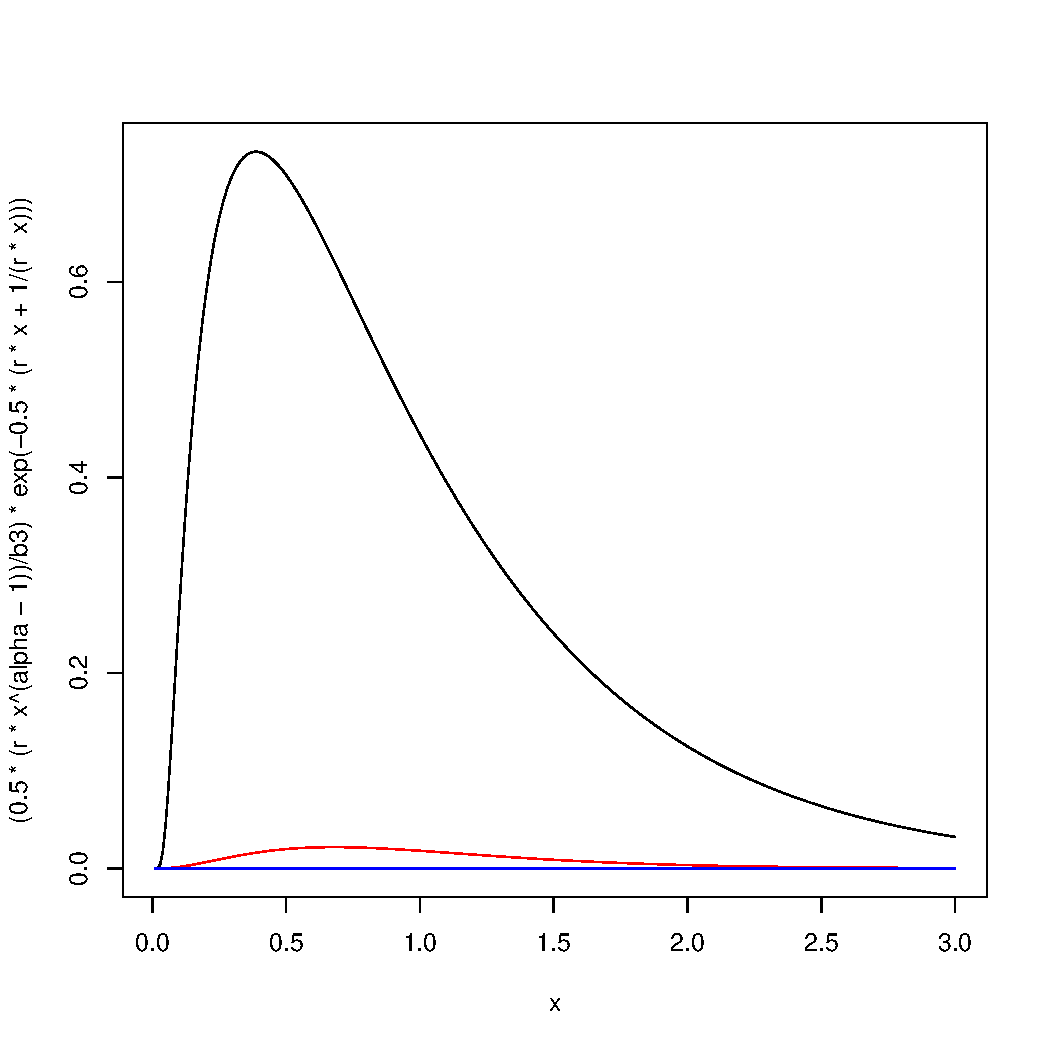
\includegraphics[width=4.0in]{fig1_freitas_frery_2005.pdf}
	\caption{Gráficos da referência \cite{ffc} para as equações (\ref{eqn99}) para $\omega=1$ e $\alpha\in(1.1,3,10,20)$.}
\label{fig5}
\end{figure}

A figura (\ref{fig6}) mostra os gráficos da equação (\ref{eqn99}) para $\alpha=1$ e diferentes valores de $\omega\in(1,2,10,30)$. 

\begin{figure}[!htb]
\centering
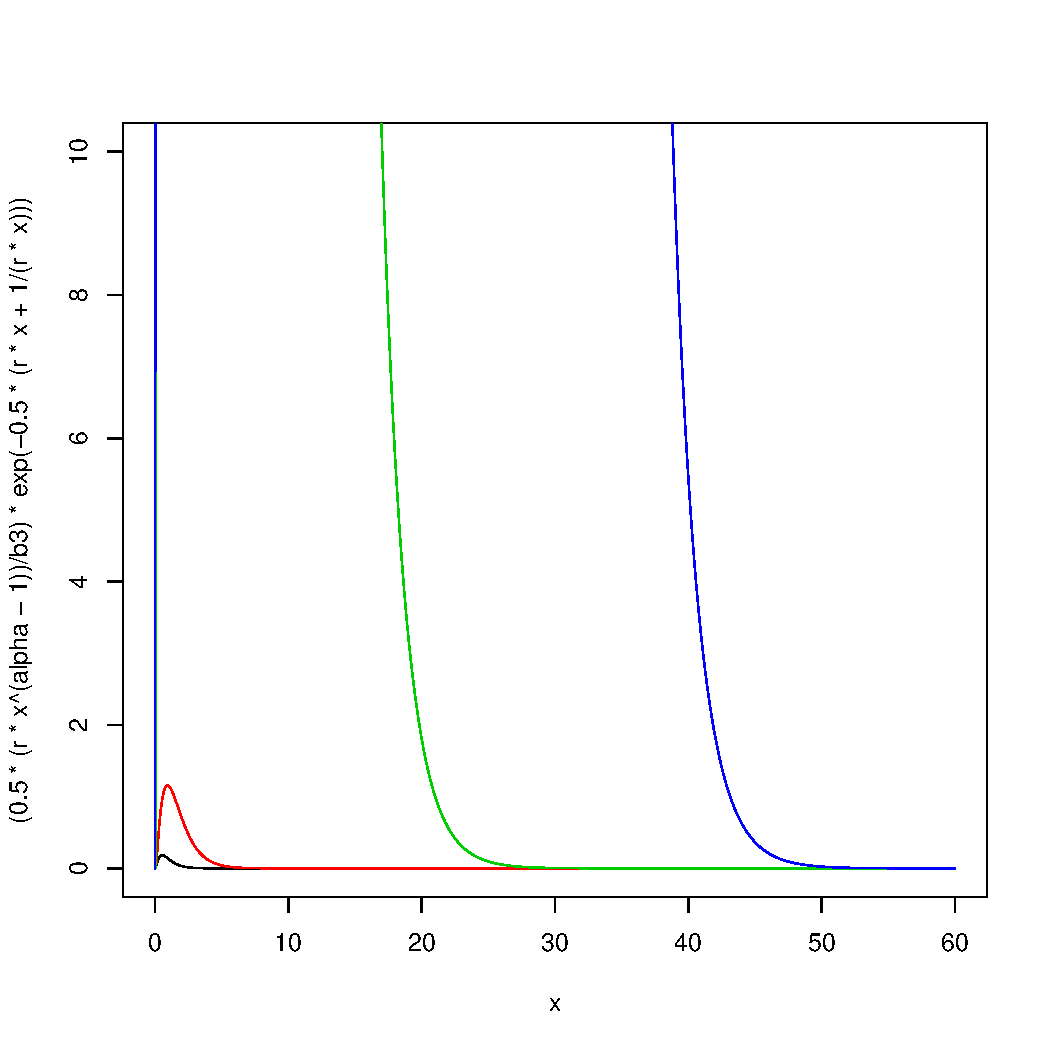
\includegraphics[width=4.0in]{fig2_freitas_frery_2005.pdf}
	\caption{Gráficos da referência \cite{ffc} para as equações (\ref{eqn99}) para $\alpha=1$ e $\omega\in(1,2,10,30)$.}
\label{fig6}
\end{figure}

	
As figuras (\ref{fig5}) e (\ref{fig6}) deste estudo deveriam estar equivalentes as figuras (1) e (2) do artigo \cite{ffc}, porém mostraram diferenças consideráveis nas magnitudes das funções. 

Para gerar as figuras (\ref{fig4}), (\ref{fig5}) e (\ref{fig6}) usei a função de Bessel (besselk) programada no pacote R.

{\bf obs 2} - Programa {\it probesselfreitasfrery2005.r} armazenado no meu computador pessoal.

{\bf obs 3} - Programa {\it profig1freitasfrery2005.r} armazenado no meu computador pessoal.

{\bf obs 4} - Programa {\it profig2freitasfrery2005.r} armazenado no meu computador pessoal.

A densidade que caracteriza a distribuição gamma com média unitária

\begin{equation}\label{eqn100}
	f_{X}(x)=\frac{\alpha^{\alpha}x^{\alpha-1}}{\Gamma(\alpha)}\exp\left(-\alpha x\right), 
\end{equation}

onde $\alpha$,$x>0$, cujos gráficos estão na figura (\ref{fig7}).

\begin{figure}[!htb]
\centering
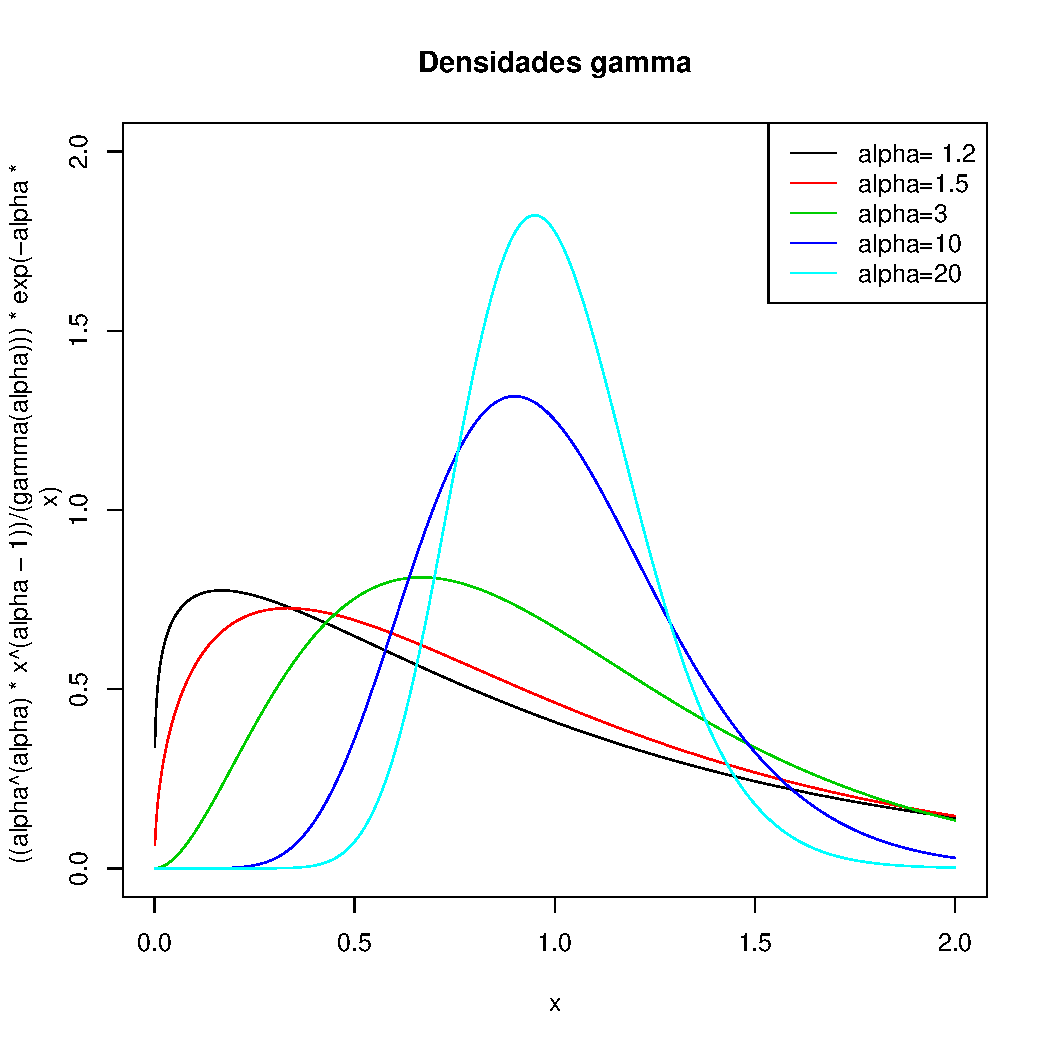
\includegraphics[width=4.0in]{fig3a_freitas_frery_2005.pdf}
	\caption{Densidades  gamma unitária (\ref{eqn100}) para $\alpha > 0$ e $|\alpha|\in(1.2,1.5,3,10,20)$, referência \cite{ffc} .}
\label{fig7}
\end{figure}


A densidade que caracteriza a distribuição gamma recíproca com média unitária

\begin{equation}\label{eqn101}
	f_{X}(x)=\frac{x^{\alpha-1}}{(-\alpha-1)^{\alpha}\Gamma(-\alpha)}\exp\left(\frac{\alpha+1}{x}\right), \\
\end{equation}

onde $-\alpha$,$x>0$, cujos gráficos estão na figura (\ref{fig8}).

\begin{figure}[!htb]
\centering
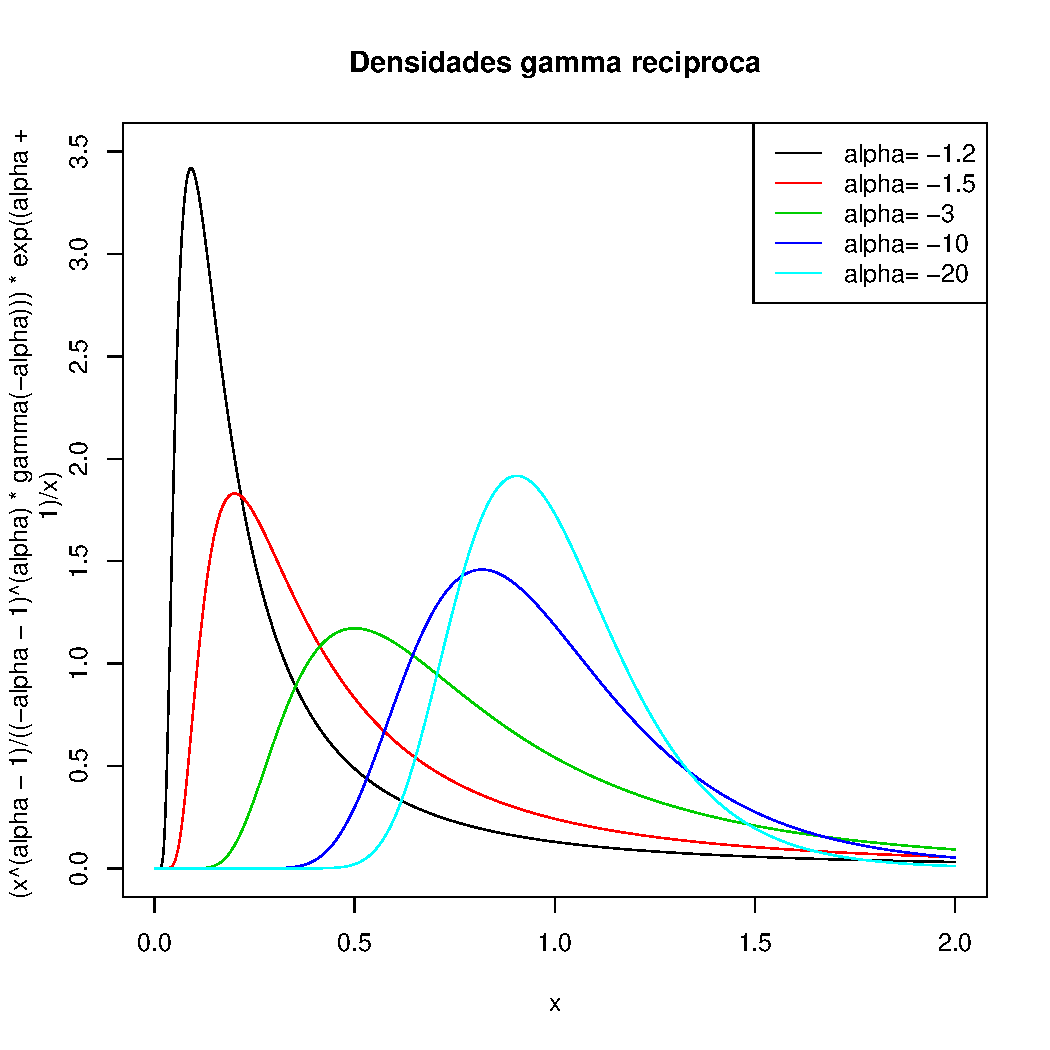
\includegraphics[width=4.0in]{fig3b_freitas_frery_2005.pdf}
	\caption{Densidades gamma unitária recíproca (\ref{eqn101}) para $\alpha < 0$ e $|\alpha|\in(1.2,1.5,3,10,20)$, referência \cite{ffc} .}
\label{fig8}
\end{figure}

{\bf obs 5} - Programa {\it profig3afreitasfrery2005.r} armazenado no meu computador pessoal.

{\bf obs 6} - Programa {\it profig3bfreitasfrery2005.r} armazenado no meu computador pessoal.

\subsection{Estudo do artigo  \cite{fmcs}}

No artigo é apresentado uma nova classe de distribuíções ${\it g}$ surgindo do modelo multiplicativo e um caso especial chamado {\it $g^{0}$} o qual se mostrou hábil para modelar  {\it extremely heterogeneus clutter}.


\subsubsection{O modelo multiplicativo e o ruído {\it speckle}}

Os ruídos {\it speckle} são associados a cenas "coerentes iluminadas" tais como as obtidas por microondas, laser, ultrasonografia, etc. É um tipo de ruído que apareçe devido a fenomênos de interferência entre o sinal incidente e o sinal refletido. Este tipo de ruído pode tornar a tarefa de interpretar a imagem tanto visual como automática difícil. 

O modelo multiplicativo é uma ferramenta usada para explicar o comportamento estatístico de dados obtidos com coerentes iluminação. Assumindo que a observação com estas imagens são o resultado do produto de duas independentes variáveis randômicas, uma $(X)$ modelando o retroespalhamento do terreno, e outra $(Y)$ modelando o ruído {\it speckle}. O primeiro é considerado real e positivo, enquanto o segundo pode ser complexo.

O valor observado é resultado da variável randômica definida como $Z=X\cdot Y$. Serão definidos os seguintes subescritos $C$, $I$, e $A$ para a referência a complexos, intensidade e amplitude respectivamente.

{\it Speckle} complexo tem distribuição normal bivariada com componentes distribuída identicamente independente tendo média $0$ e variância $\frac{1}{2}$. Assim, $\mathbf{Y}_{C}=(Y_{\mathbb{R}}, Y_{\mathbb{I}})\sim N2(0,\frac{1}{2})$ denota a distribuíção do par.

{\it Multilook intensity speackle} surge tomando a média sobre $n$ amostras independentes de $Y_{I}=\|Y_{C}\|^2$ na qual implica a distribuição gamma denotada por $Y_{I}\sim \Gamma(n,n)$ e caracterizado pela densidade mostrada na figura (\ref{fig9})

\begin{equation}\label{eqn102}
	f_{Y_{I}}(y)=\frac{n^{n}}{\Gamma(n)}y^{n-1}\exp\left(-ny\right),\quad y,n>0 
\end{equation}

\begin{figure}[!htb]
\centering
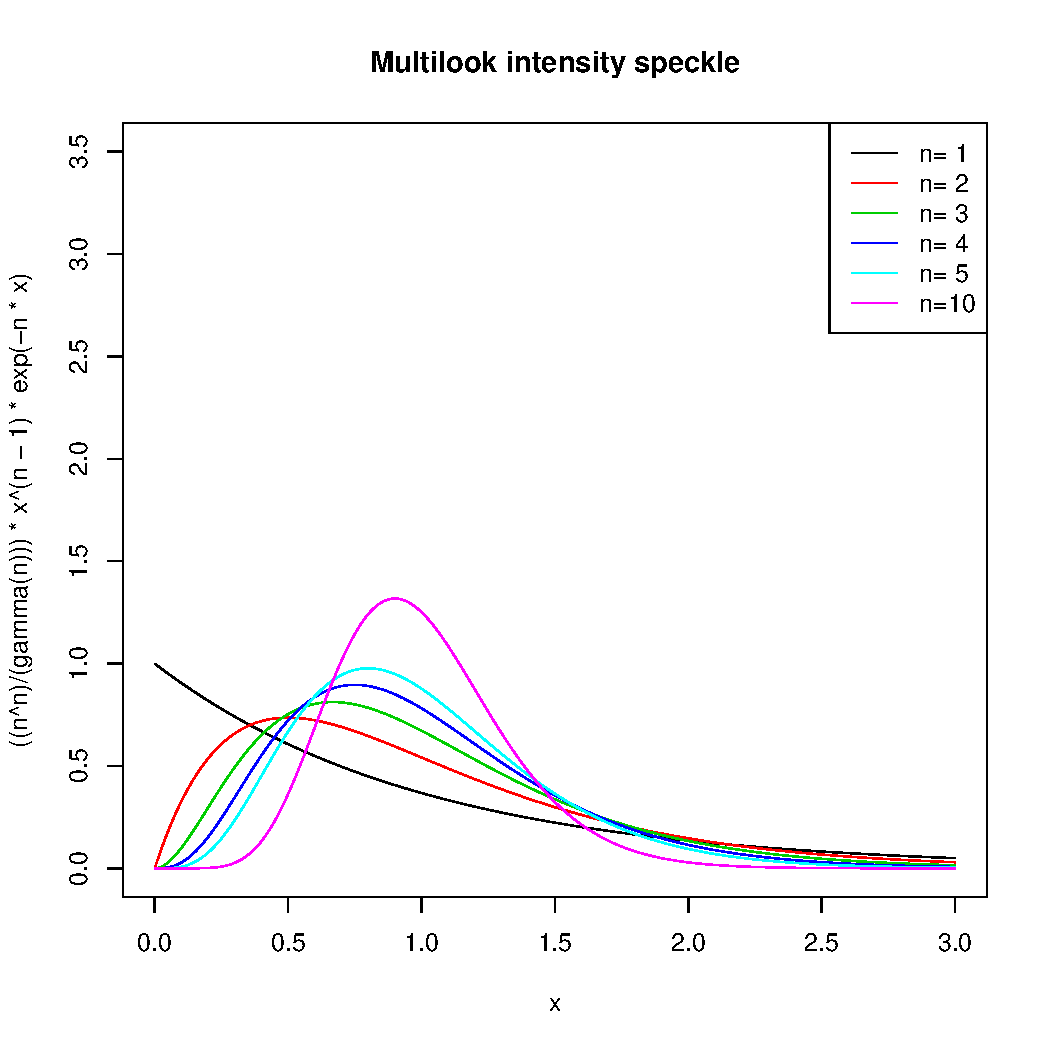
\includegraphics[width=4.0in]{fig_eq_fyi_frery_muller_1997.pdf}
	\caption{Multilook Intensity speckle  para $n\in(1,2,3,4,5,10)$.}
\label{fig9}
\end{figure}

{\it Multilook amplitude speackle} surge tomando a raíz quadrada do {\it Multilook intensity speackle} e portanto a raíz quadrada da distribuíção gamma, denotado por $Y_{A}\sim \Gamma^{\frac{1}{2}}(n,n)$ e caracterizado pela densidade e mostrada na figura  (\ref{fig10}).

\begin{equation}\label{eqn103}
	f_{Y_{A}}(y)=\frac{2n^{n}}{\Gamma(n)}y^{2*n-1}\exp\left(-ny^2\right),\quad y,n>0 
\end{equation}
\begin{figure}[!htb]
\centering
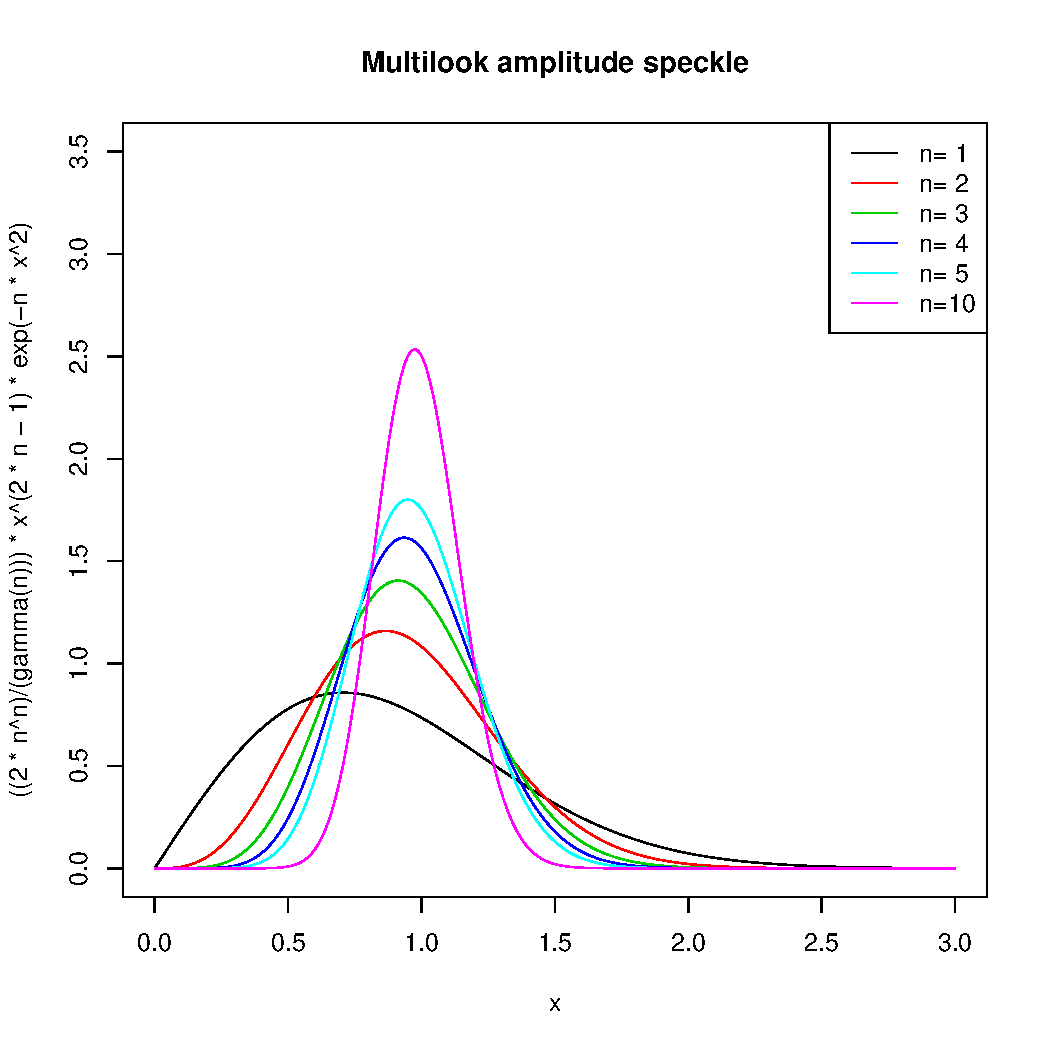
\includegraphics[width=4.0in]{fig_eq_fya_frery_muller_1997.pdf}
	\caption{Multilook Amplitude speckle  para $n\in(1,2,3,4,5,10)$.}
\label{fig10}
\end{figure}
\subsubsection{Amplitude do retroespalhamento}

A amplitude do retroespalhamento obedeçe a raíz quadrada da lei gaussiana inversa generalizada, donotado aqui por $\mathbf{X}_{A}\sim N^{-\frac{1}{2}}(\alpha,\gamma,\lambda)$, sendo sua densidade dada por
\begin{equation}\label{eqn104}
	f_{X_{A}}(x)=\frac{\left(\frac{\lambda}{\gamma}\right)^{\frac{\alpha}{2}}}{K_{\alpha}(2\sqrt{\lambda\gamma})}x^{2\alpha-1}\exp\left(-\frac{\gamma}{x^2}-\lambda x^2\right) 
\end{equation}

Dois casos particulares desta distribuíção são de interesse na análise de dados $SAR$, a raíz quadrada de gamma e a recíproca da raíz quadrada da distribuição gamma. 

A raíz quadrada da distribuição gamma surge quando $\gamma \rightarrow 0$ enquanto $\alpha,\lambda>0$. Esta distribuição é denota aqui por $\Gamma^{\frac{1}{2}}(\alpha,\lambda)$ e caracterizada pela densidade 
\begin{equation}\label{eqn105}
	f_{X_{A}}(x)=\frac{2\lambda^{\alpha}}{\Gamma(\alpha)}x^{2\alpha-1}exp(-\lambda x^2), \quad \alpha,\lambda, x>0. 
\end{equation}
A recíproca da raíz quadrada da distribuição gamma surge quando $\lambda\rightarrow 0$ enquanto $-\alpha,\gamma>0$. Esta distribuição é denotada aqui por $\Gamma^{-\frac{1}{2}}(\alpha,\gamma) $ e caracterizada pela densidade
\begin{equation}\label{eqn106}
	f_{X_{A}}(x)=\frac{2}{\gamma^{\alpha}\Gamma(-\alpha)}x^{2\alpha-1}exp(-\frac{-\gamma}{x^2}), \quad -\alpha,\lambda, x>0. \\
\end{equation}

\subsubsection{Retorno complexo}

Definindo uma distribuição geral $X_{A}$ como sendo $N^{-\frac{1}{2}}$ e dado um ruído complexo {\it speckle} é definido como $Y_{C}=(Y_{\mathbb{R}},Y_{\mathbb{I}})\sim N2(0,\frac{1}{2})$. assim é possível derivar uma distribuição marginal associada para o retorno complexo, o qual é dado por $Z_{C}=X_{A}\cdot Y_{C}=X_{
A}\cdot(Y_{\mathbb{R}},Y_{\mathbb{I}})$. A densidade que caracteriza a distribuição da parte real e da parte imaginária de $Z_{C}$, denotada por $Z_{\circ}$ e definida por
\begin{equation}\label{eqn107}
	f_{Z_{\circ}}(x)=\frac{1}{K_{\alpha}(2\sqrt{\lambda\gamma})}\sqrt{\frac{\left(\frac{\lambda}{\gamma} \right)^{\alpha}}{\pi}}\left(\frac{\gamma+x^2}{\lambda} \right)^{\frac{\alpha-\frac{1}{2}}{2}}K_{\alpha-\frac{1}{2}}\left(2\sqrt{\lambda(\gamma+x^2)}\right), x\in\mathbb{R}. 
\end{equation}

sendo o espaço do parâmetro dado por:
\begin{equation}\label{eqn108}
	\left\{
\begin{array}{ccr}
	\gamma>0,&\lambda\geq 0&\mbox{se}\quad\alpha<0 \\
	\gamma>0,&\lambda > 0&\mbox{se}\quad\alpha=0 \\
	\gamma\geq0,&\lambda> 0&\mbox{se}\quad\alpha>0 \\
\end{array}
\right.
\end{equation}

Esta distribuição é denotada por $g_{C}(\alpha,\gamma,\lambda)$, o artigo mostra que a distribuição $g_{C}(\alpha,\gamma,\lambda)$ pode convergir em distribuição com condições estabelecidas no artigo para $K){C}(\alpha,\lambda)$(retroespalhamento heterogêneo) ou para $g_{C}^{0}$ (retroespalhamento extremamente heterogêneo).

A distribuição $K$ e $g^0$ podem ser representadas pelas equações respectivamente

\begin{equation}\label{eqn109}
	f_{Z_{\circ}}(x)=\frac{2}{\Gamma(\alpha)}\sqrt{\frac{\lambda^{\alpha+\frac{1}{2}}}{\pi}} |x|^{\alpha-\frac{1}{2}}K_{\alpha-\frac{1}{2}}(2|x|\sqrt{\lambda}), \alpha,\lambda>0, x\in\mathbb{R}. \\
\end{equation}
\begin{equation}\label{eqn110}
	f_{Z_{\circ}}(x)=\frac{\Gamma(\frac{1}{2}-\alpha)}{\sqrt{\pi}\gamma^{\alpha}\Gamma(-\alpha)}\left(x^2+\gamma\right)^{\alpha-\frac{1}{2}}, -\alpha,\lambda>0, x\in\mathbb{R}. 
\end{equation}

\subsubsection{Retorno da amplitude}

A distribuição do retorno da distribuição surge de $Z_{A}=X_{A}Y_{A}$ onde $X_{A}\sim N^{-\frac{1}{2}}(\alpha,\gamma,\lambda)$  e $Y_{A}\sim\Gamma^{\frac{1}{2}}(n,n)$ é denotado por como $g_{A}(\alpha,\gamma,\lambda,n)$ é caracterizado pela densidade  

\begin{equation}\label{eqn111}
	f_{Z_{\circ}}(x)=\frac{2n^n\left(\frac{\lambda}{\gamma}\right)^{\frac{\alpha}{2}}}{\Gamma(n)K_{\alpha}(2\sqrt{\lambda\gamma})}x^{2n-1}\left(\frac{\gamma+nx^2}{\lambda}\right)^{\frac{\alpha-n}{2}}K_{\alpha-n}(2\sqrt{\lambda(\gamma+nx^2)}), x\in\mathbb{R}. \\
\end{equation}
com o espaço de parametro (\ref{eqn108}).

Onde $K_{A}$ e $g_{A}$  distribuição amplitude $K$ e a distribuição $g^0$ e podem ser representadas pelas equações abaixo respectivamente

\begin{equation}\label{eqn112}
	f_{Z_{A}}(x)= \frac{4\lambda n x}{\Gamma(\alpha)\Gamma(n)}(\lambda n x^2)^{\frac{(\alpha+n)}{2}-1} K_{\alpha-n}(2x\sqrt{\lambda n}), \alpha,\lambda,n, x>0. 
\end{equation}

\begin{equation}\label{eqn113}
	f_{Z_{A}}(x)= \frac{2n^n\Gamma(n-\alpha)\gamma^{-\alpha}x^{2n-1}}{\Gamma(n)\Gamma(-\alpha)(\gamma+nx^2)^{n-\alpha}}, -\alpha,\gamma,n, x>0. 
\end{equation}


As distribuições $g_A$ com a variação do parâmetros conforme o artigo estão representadas nas figuras (\ref{fig11}) e (\ref{fig12}).


\begin{figure}[!htb]
\centering
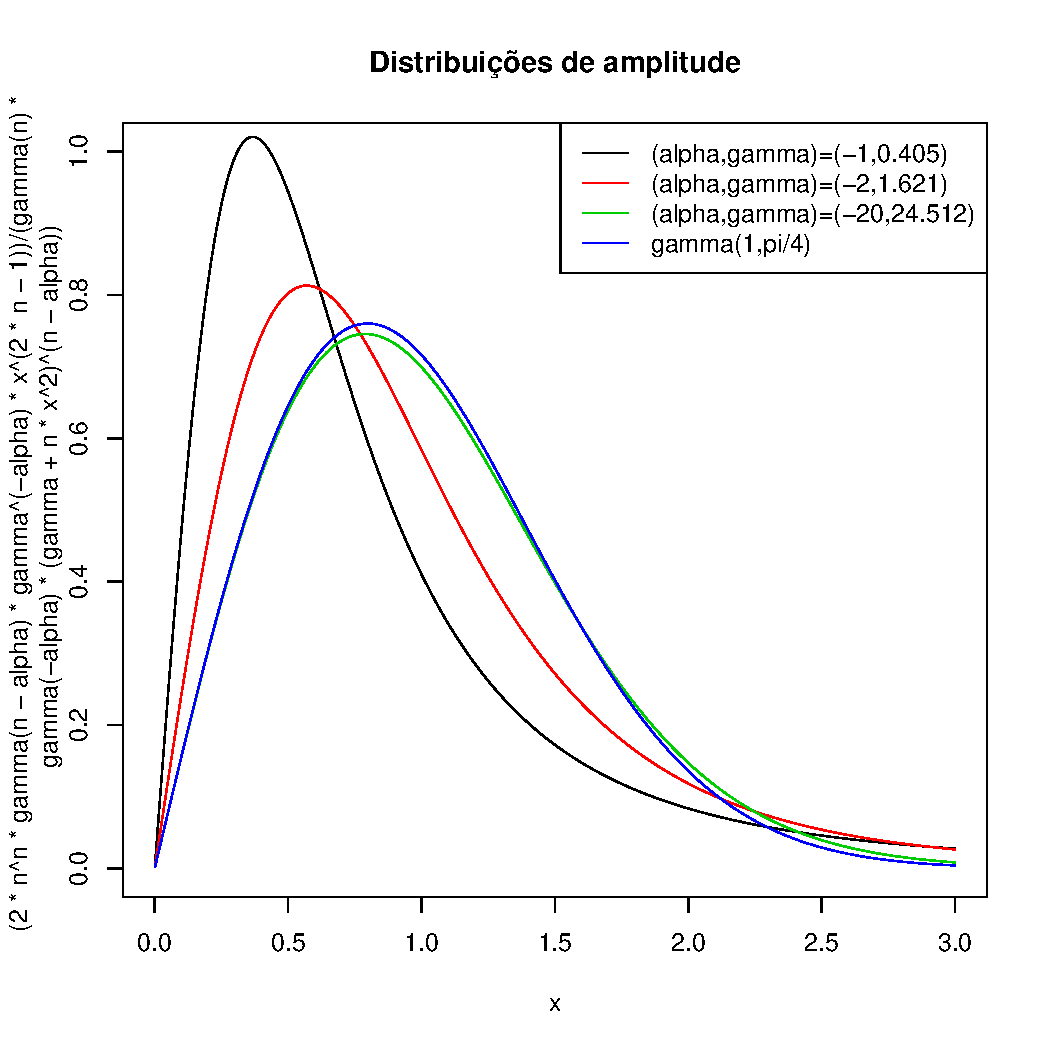
\includegraphics[width=4.0in]{fig_eq_ga_fig1_frery_muller_1997.pdf}
	\caption{Distribuições de amplitude.}
\label{fig11}
\end{figure}

\begin{figure}[!htb]
\centering
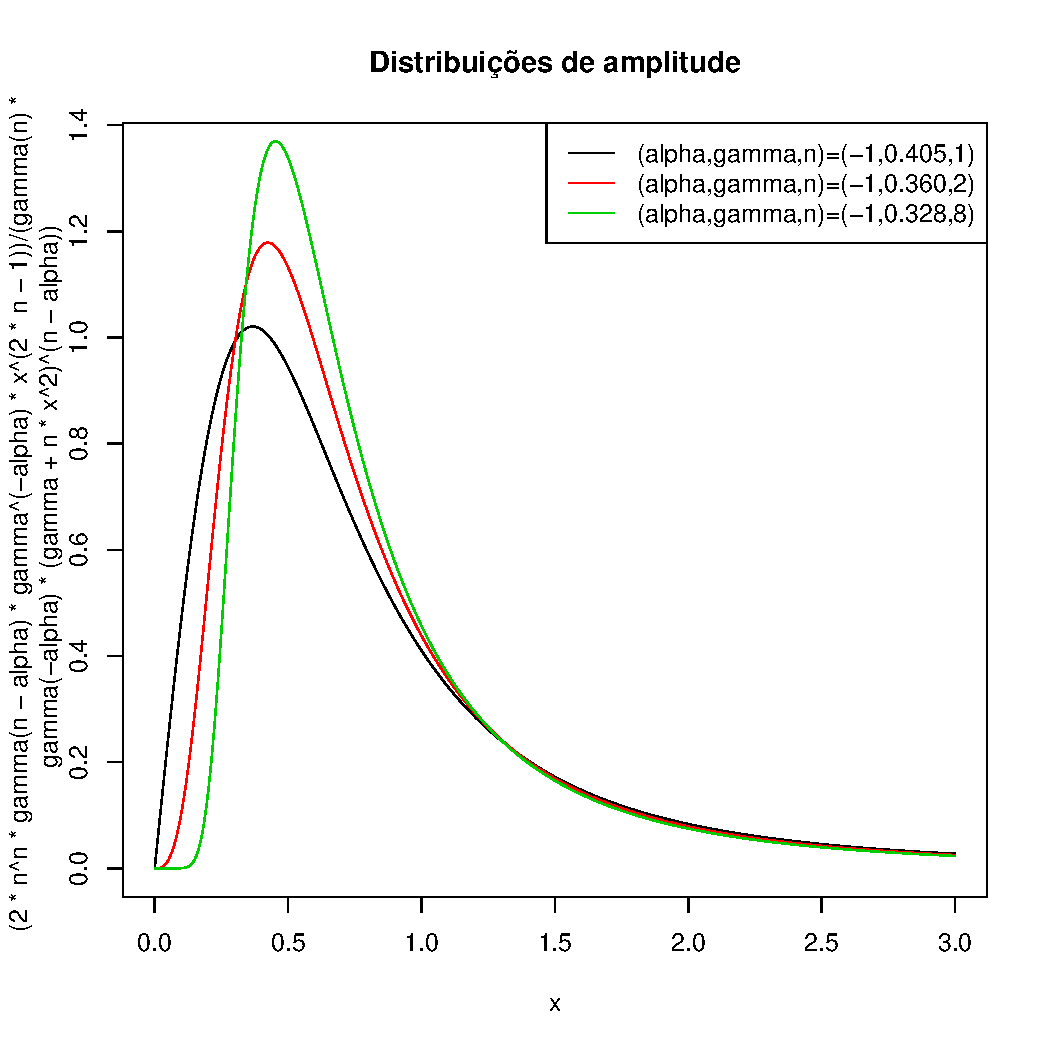
\includegraphics[width=4.0in]{fig_eq_ga_fig2_frery_muller_1997.pdf}
	\caption{Distribuições de amplitude.}
\label{fig12}
\end{figure}

\subsubsection{Modelando áreas urbanas}

Quando estimamos os três parâmetros da distribuíção $g_A$ sobre áreas urbanas foi observado que o atrator e a solução global do sistema de equações estava  no subconjunto do espaço de parâmetros dado por ($\alpha<0,\gamma0,\lambda<10^{-6}$); 

\subsection{Estudo do artigo  \cite{fnc}}.

\subsubsection{Distribuição complexa de Wishart}

\begin{equation}\label{eqn114}
	f_{\mathbf{Z}}(\mathbf{Z};\mathbf{\Sigma},L)=\frac{L^{pL}|\mathbf{Z}|^{L-p}}{|\mathbf{\Sigma}|^{L}\Gamma_d(L)} exp(-L\mathrm{tr}{(\mathbf{\Sigma}^{-1}\mathbf{Z})}), \\
\end{equation}

A ideia é encontrar a derivada do logaritmo natural em relação ao número de {\it looks}, com esse intuito a distribuição (\ref{eqn114}) será reescrita
\begin{equation}\label{eqn115}
\begin{array}{ccc}
	\ln{\left(f_{\mathbf{Z}}(\mathbf{Z};\mathbf{\Sigma},L)\right)}&=&\ln{\left(\frac{L^{pL}|\mathbf{Z}|^{L-p}}{|\mathbf{\Sigma}|^{L}\Gamma_d(L)} \exp(-L\mathrm{tr}{(\mathbf{\Sigma}^{-1}\mathbf{Z})})\right)}, \\
	\ln{\left(f_{\mathbf{Z}}(\mathbf{Z};\mathbf{\Sigma},L)\right)}&=&\ln{\left(\frac{L^{pL}|\mathbf{Z}|^{L-p}}{|\mathbf{\Sigma}|^{L}\Gamma_d(L)}\right)}\ln{\left( exp(-L\mathrm{tr}{(\mathbf{\Sigma}^{-1}\mathbf{Z})})\right)}, \\
	\ln{\left(f_{\mathbf{Z}}(\mathbf{Z};\mathbf{\Sigma},L)\right)}&=&\ln{\left(L^{pL}|\mathbf{Z}|^{L-p}\right)} - \ln{\left(|\mathbf{\Sigma}|^{L}\Gamma_d(L)\right)}-L\mathrm{tr}{(\mathbf{\Sigma}^{-1}\mathbf{Z})}, \\
	\ln{\left(f_{\mathbf{Z}}(\mathbf{Z};\mathbf{\Sigma},L)\right)}&=&\ln{\left(L^{pL}\right)}+\ln{\left( |\mathbf{Z}|^{L-p}\right)} - \ln{\left(|\mathbf{\Sigma}|^{L}\right)}-\ln{\left(\Gamma_d(L)\right)}-L\mathrm{tr}{(\mathbf{\Sigma}^{-1}\mathbf{Z})}, \\
	\ln{\left(f_{\mathbf{Z}}(\mathbf{Z};\mathbf{\Sigma},L)\right)}&=&pL\ln{\left(L\right)}+(L-p)\ln{\left( |\mathbf{Z}|\right)} - L\ln{\left(|\mathbf {\Sigma}|\right)}-\ln{\left(\Gamma_d(L)\right)}-L\mathrm{tr}{(\mathbf{\Sigma}^{-1}\mathbf {Z})}, \\
	\ln{\left(f_{\mathbf{Z}}(\mathbf{Z};\mathbf{\Sigma},L)\right)}&=&pL\ln{\left(L\right)}+L\ln{\left( |\mathbf{Z}|\right)}-p\ln{\left( |\mathbf{Z}|\right)}- L\ln{\left(|\mathbf{\Sigma}|\right)}-\ln{\left(\Gamma_d(L)\right)}-L\mathrm{tr}{(\mathbf{\Sigma}^{-1}\mathbf {Z})}, \\
\end{array}
\end{equation}


Derivando com relação ao número de {\it looks} $L$, teremos

\begin{equation}\label{eqn116}
	{\footnotesize
\begin{array}{ccc}
	\frac{\partial}{\partial L}\left(\ln{\left(f_{\mathbf{Z}}(\mathbf{Z};\mathbf{\Sigma},L)\right)}\right)&=&\frac{\partial}{\partial L}\left(pL\ln{\left(L\right)}+L\ln{\left( |\mathbf{Z}|\right)}-p\ln{\left( |\mathbf{Z}|\right)} - L \ln{\left(|\mathbf{\Sigma}|\right)}-\ln{\left(\Gamma_d(L)\right)}-L\mathrm{tr}{(\mathbf{\Sigma}^{-1}\mathbf{Z})}\right), \\
	\frac{\partial}{\partial L}\left(\ln{\left(f_{\mathbf{Z}}(\mathbf{Z};\mathbf{\Sigma},L)\right)}\right)&=&\left(p\ln{\left(L\right)}+p\right)+\ln{\left( |\mathbf{Z}|\right)} - \ln{\left(|\mathbf{\Sigma}|\right)}-\frac{\partial}{\partial L}\ln{\left(\Gamma_d(L)\right)}-\mathrm{tr}{(\mathbf{\Sigma}^{-1}\mathbf{Z})}, \\
	\frac{\partial}{\partial L}\left(\ln{\left(f_{\mathbf{Z}}(\mathbf{Z};\mathbf{\Sigma},L)\right)}\right)&=&p\left(\ln{\left(L\right)}+1\right)+\ln{\left(\frac{|\mathbf{Z}|}{|\mathbf{\Sigma|}}\right)}-\frac{\Gamma^{\prime}_d(L)}{\Gamma_d(L)}-\mathrm{tr}{(\mathbf{\Sigma}^{-1}\mathbf{Z})}. \\
\end{array}}
\end{equation}

Sendo $n$ tomado arbitrariamente entre o $L$ {\it looks} temos a seguinte equação
\begin{equation}\label{eqn117}
	\frac{\partial}{\partial n}\left(\ln{\left(f_{\mathbf{Z}}(\mathbf{Z};\mathbf{\Sigma},n)\right)}\right)=p\left(\ln{\left(n\right)}+1\right)+\ln{\left(\frac{|\mathbf{Z}|}{|\mathbf{\Sigma|}}\right)}-\frac{\Gamma^{\prime}_d(n)}{\Gamma_d(n)}-\mathrm{tr}{(\mathbf{\Sigma}^{-1}\mathbf{Z})}. 
\end{equation}


\subsection{Estudo do livro  \cite{lp}}.

Algumas observações:
\begin{description}
\item[(1)] As imagens $SAR$ são uma técnica de sensoriamento remoto bem desenvolvidas para obter imagens da superfície da terra bidimensionais com alta resolução espacial e em larga escla.
\item[(2)] Sistema de imagem $SAR$ são um sistema de radar operando na região de microondas do spectro eletromagnético, usualmente entre a $P-${\it band} e $Ka-${\it band} conforme tabela abaixo.

\begin{center}
	\begin{table}[h!]
		\centering
\begin{tabular}{ |c|c|c|c| } 
\hline
	{\it band} & Frequência$f(Ghz)$ & Freq$\times$Comprimento de onda $\lambda(cm)$. \\
\hline
	$P-${\it band}&$(<0.39, 0.39)$  & $0.3\times 100.0$  \\ 
	$L-${\it band}&$(0.39-1.55)$  &  $1.0\times 30.0$\\ 
	$S-${\it band}&$(1.55-3.90)$  &  $3.0\times 10.0$\\ 
	$C-${\it band}&$(3.90-5.75)$  & $\sim(4.0\times 7.0)$ \\ 
	$X-${\it band}&$(5.75-10.9)$  & $10.0\times 3.0$ \\ 
	$K-${\it band}&$(10.9-36.0)$  & $30.0\times 1.0$ \\ 
	$Q-${\it band}&$(36.0-46.0)$  & $\sim(40.0\times 0.8 )$ \\ 
	$V-${\it band}&$(46.0-56.0)$  & $\sim(50.0\times 0.6)$ \\ 
	$W-${\it band}&$(56.0- >56.0)$  & $100.0\times 0.3$ \\ 
\hline
\end{tabular}
	\caption{Espectro magnético para a faixa de microondas.}
	\label{sec8tab01}
\end{table}
\end{center}
\item[(3)] O radar é usualmente montado em uma plataforma em movimento(aviões, satélites e etc...) e opera com a fonte eletromagnética emissora perpendicular ao linha suporte do voo.
\item[(4)] O sistema emite para terra um pulso de microondas e recebe um sinal eletromagnético retroespalhados.
\item[(5)] O sistema $SAR$ usa o sinal recebido para sintetizar a imagem da superfície terra com alta resolução.  
\item[(6)] E ainda permite monitorar clima em escala global quando a frequência opera abaixo de $L-${\it band}.  

\end{description}

\subsubsection{Estudo das imagens Polsar }

\begin{figure}[hbt]
\begin{minipage}[b]{0.450\linewidth}
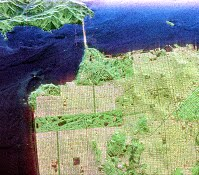
\includegraphics[width=\linewidth]{polsar_teste.jpeg}
\caption{Imagem Polsar da Baía de São Francisco.}
\label{fig5:sobel}
\end{minipage}\hfill
\begin{minipage}[b]{0.450\linewidth}
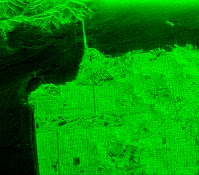
\includegraphics[width=\linewidth]{polsar_green.jpeg}
\caption{Canal com a cor verde da imagem Polsar.}
\label{fig5:Log}
\end{minipage}
\end{figure}

\begin{figure}[!htb]
\begin{minipage}[b]{0.450\linewidth}
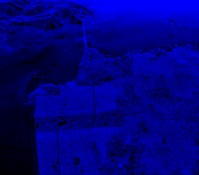
\includegraphics[width=\linewidth]{polsar_blue.jpeg}
\caption{Canal com a cor azul da imagem Polsar.}
\label{fig5:sobel}
\end{minipage}\hfill
\begin{minipage}[b]{0.450\linewidth}
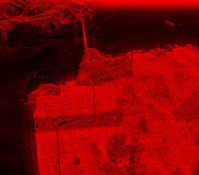
\includegraphics[width=\linewidth]{polsar_red.jpeg}
\caption{Canal com a cor vermelha da imagem Polsar.}
\label{fig5:Log}
\end{minipage}
\end{figure}

\subsection{Estudo do artigo  \cite{gamf}}
\subsubsection{Imagens Simuladas}

Será usado imegens sintéticas $500 \times 500$ para estudar a acurária de diferentes métodos de classificação. A ideia é estudar como ocorre a redução de ruído e preservação de bordas. Para gerar uma imagem PolSAR usaremos a imagem sintética combinada com as matrizes de covariância $\{\Sigma_{k}\}_{k=1\dots5}$ extraídas de uma imagem PolSAR com uma distribuição de Wishart complexa $W_G(\Sigma, L)$. No presente artigo os experimentos apresentados usam $L=4$.

Para cada par de matrizes de covariância $\Sigma_{k_1}$, $\Sigma_{k_2}$ (com $k_2>k_1$) será gerado uma imagem PolSAR $P_{k_1,k_2,\beta}$ da seguinte maneira: em cada pixel branco da imagem sintética vindo de $W_G(\Sigma_{k_1}, L)$ e de cada pixel preto vindo de $W_G(\Sigma_{k_2},L)$ vamos fazer a combinação linear $W_G(\beta\Sigma_{k_1}+(1-\beta)\Sigma_{k_2}, L)$ com $\beta\in[0,1]$.

O parâmetro $\beta$ é usado para pesar as informações entre as matrizes de covariância $\Sigma_{k_1}$ e $\Sigma_{k_2}$, modelando a mistura de classes em imagens PolSAR atuais. Quando $\beta=0$ não há mistura e o problema consiste em escolher entre amostras puras de $\Sigma_{k_1}$ e $\Sigma_{k_2}$. Se o parâmetro $\beta$ se aproxima de $1$, teremmos uma aproximação com a matriz de covariância $\Sigma_{k_1}$, assim teremos maior dificuldade de escolher classes. As figuras abaixo mostram algumas {\it Phantons} geradas com auxílio dos códigos programados pelos autores do artigo em Matlab e localizado em  \begin{verbatim} http://www.ctim.es/polsar/\end{verbatim}

\begin{figure}[!htb]
\minipage{0.32\textwidth}
  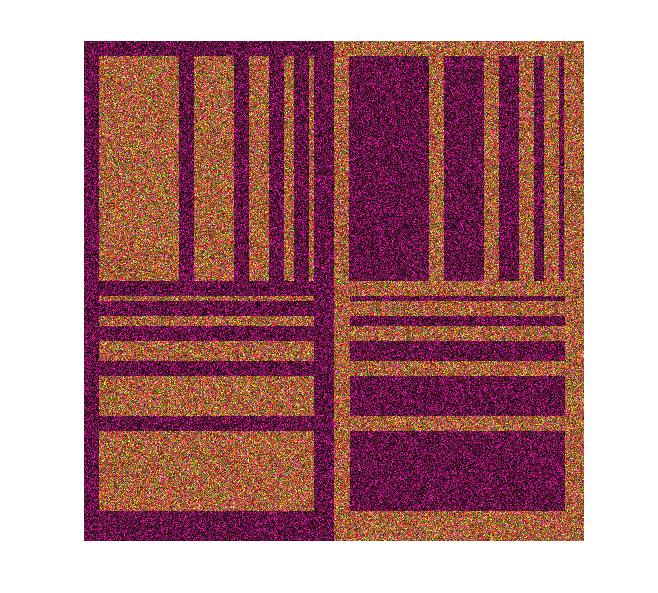
\includegraphics[width=\linewidth]{Eq_Phantom_0p000_1_3_1.jpg}
	\caption{$P_{1,3,0.0}$}\label{fig:awesome_image1}
\endminipage\hfill
\minipage{0.32\textwidth}
  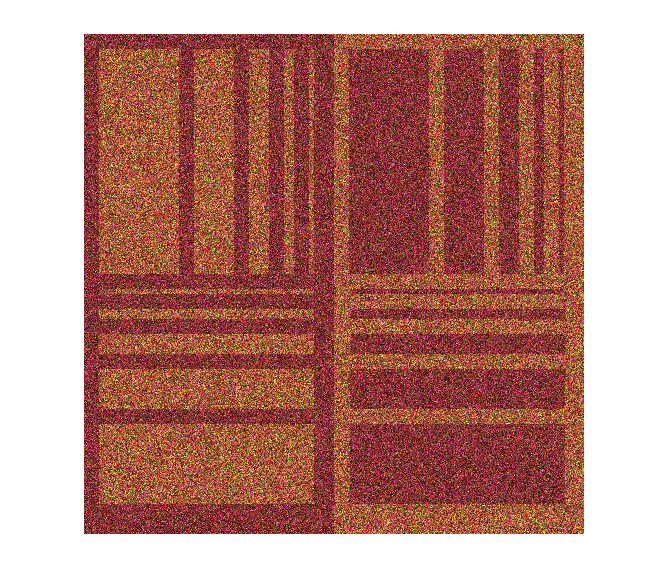
\includegraphics[width=\linewidth]{Eq_Phantom_0p500_1_3_1.jpg}
	\caption{$P_{1,3,0.5}$}\label{fig:awesome_image1}
\endminipage\hfill
\minipage{0.32\textwidth}%
  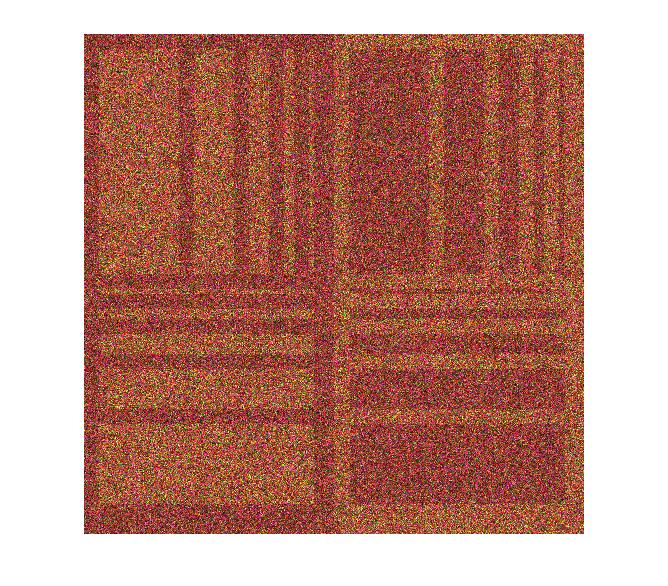
\includegraphics[width=\linewidth]{Eq_Phantom_0p700_1_3_1.jpg}
	\caption{ $P_{1,3,0.7}$}\label{fig:awesome_image1}
\endminipage
%\caption{A really Awesome Image}\label{fig:awesome_image3}
\end{figure}

As {\it Phantons} foram geradas com o auxílio do método Monte Carlo, 
% % % Os phantoms são um elemento de um estudo Monte Carlo
que será descrito com mais detalhes na próxima seção.

\subsubsection{Monte Carlo \cite{odell}}

Sendo uma matriz de covariância e simétrica definida positiva $S$. Portanto podemos encontrar a fatoração de Crout $S=CC^H$. Segue que o vetor $Z_{\alpha}$ pode ser encontrado da seguinte maneira $Z_{\alpha}=CW_{\alpha}$, onde o vetor $W_{\alpha}$ $p\times 1$ é distribuido como $N(\phi,I)$, isto é, $W_{\alpha}\sim N(\phi,I)$. Definindo $N(\phi,I)$ como uma distribuição normal multivariada com vetor de média nula $\phi$ e a matriz de covariância sendo a identidade $I$.Isto significa que $W_{\alpha}$ são vetores independentes $p-$dimensional cuja as componentes são variáveis independentes normalmentes distribuídas com média zero e variância unitária. 

\begin{equation}\label{eqn118}
\begin{array}{ccccc}
	B&=&\{b_{ij}\}&=&\sum_{\alpha=1}^{N-1}W_{\alpha}W_{\alpha}^{T} \\
\end{array}
\end{equation}

então

\begin{equation}\label{eqn119}
\begin{array}{ccccccc}
	CBC^{T}&=&\{b_{ij}\}&=&\sum_{\alpha=1}^{N-1}CW_{\alpha}W_{\alpha}^{T}C^{T}&=&A \\
\end{array}
\end{equation}

Desta forma, o problema fica restrito a gerar uma matriz randômica simétrica $B$.

\subsubsection{Algoritmo de geração das imagens {\it Phantons}} 

No arquivo \begin{verbatim} S_6_classes.m \end{verbatim} há seis matrizes de dados Polsar Wishart, extraídas de uma imagem de dados "inteiramente" Polsar. Por exemplo  
$$
\mathbf{S(:, :, 1)} = \left[
\begin{array}{lll}
	0.002836  &0.000067+-0.000526i &0.006216+0.000654i\\
	0.000067+0.000526i &0.000543 & -0.000084+0.001434i\\
	0.006216-0.000654i& -0.000084-0.001434i & 0.016687\\
\end{array}
\right].
$$

Além das definições de $S$ nesse arquivo temos a definição do número de visadas $L=4$. Rodando o arquivo será gerado o arquivo \begin{verbatim} S_6_classes.mat \end{verbatim} com as matrizes e o número de visadas.

No arquivo \begin{verbatim} cwishart_variates.m \end{verbatim} está programando o processo descrito na seção anterior e com uma versão melhorada, o arquivo recebe a matriz  $Sigma(:,:)$, $L$ e  $NSamples$. Onde $Sigma(:,:)$ é uma matriz de covariância $\Sigma_i$ e o número de visadas $L$ definidas respectivamente em $\mbox{S\_6\_classes.m}$ e $NSamples$ o número de amostras definido no programa.

A saída do programa é um vetor de matrizes  de Wishart $B$ com ($p\times p \times Nsample$). 


O arquivo \begin{verbatim} Generate_Polsar_two_classes_phantom \end{verbatim} tem entradas $S, L, m, n$ onde respectivamente $S$ é a matriz de covariância $\Sigma_i$, $L$ é o número de visadas, e $m$ e $n$ são as dimensões da imagem {\it Phantom}.   

A saída do programa são a imagem {\it phantom} de tamanho $(m\times n \times 9)$e uma vetor de matrizer $R$ de tamanho $(3 \times 3 \times 2)$.


O arquivo \begin{verbatim} Polsar_two_classes_phantom_Convex_Sum.m \end{verbatim} é o programa principal que chama os programas descritos acima e geram uma matriz wishart $W_G(\Sigma,L)$. Para cada par de matriz de covariância $\Sigma_{k_1}$e $\Sigma_{k_2}$ com $k_2>k_1$ será gerado uma imagem PolSAR $P_{k_1,k_2,\alpha}$ da seguinta maneira: Em casa pixel branco da imagem {\it phantom} colocamos $W_G(\Sigma_{k_1},L)$ e para cada pixel preto vamos colocar a combinação linear $W_G(\alpha\Sigma_{k_1}+(1-\alpha\Sigma_{k_2}))$ com $\alpha\in[0,1]$ combinações lineares convexas de {\it Phantons} com duas matrizes de covariância,  
 
\subsubsection{Imagens  {\it Phantons} $P_{k_1,k_2,0}$ - Visualização de Pauli} 


\textcolor{red}{Para essa imagens está sendo usado o matlab, com a visualização de Pauli}

\begin{figure}[!htb]
\minipage{0.25\textwidth}
  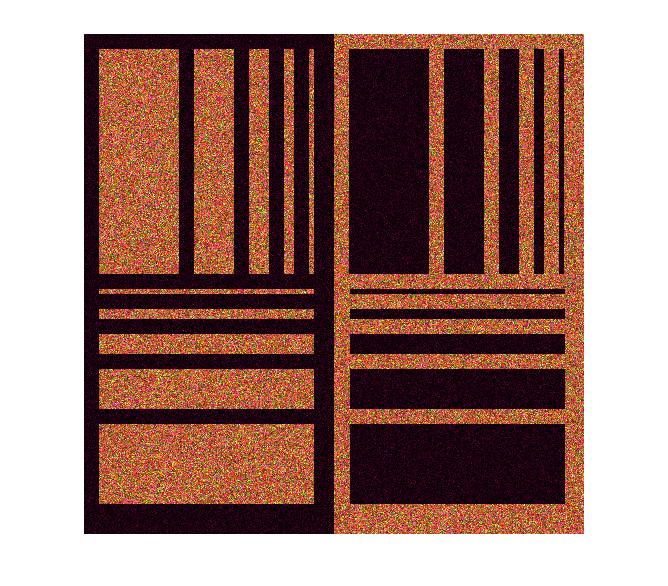
\includegraphics[width=\linewidth]{Eq_Phantom_0p000_1_2_1.jpg}
	\caption{$P_{1,2,0.0}$}\label{fig:awesome_image1}
\endminipage\hfill
\minipage{0.25\textwidth}
  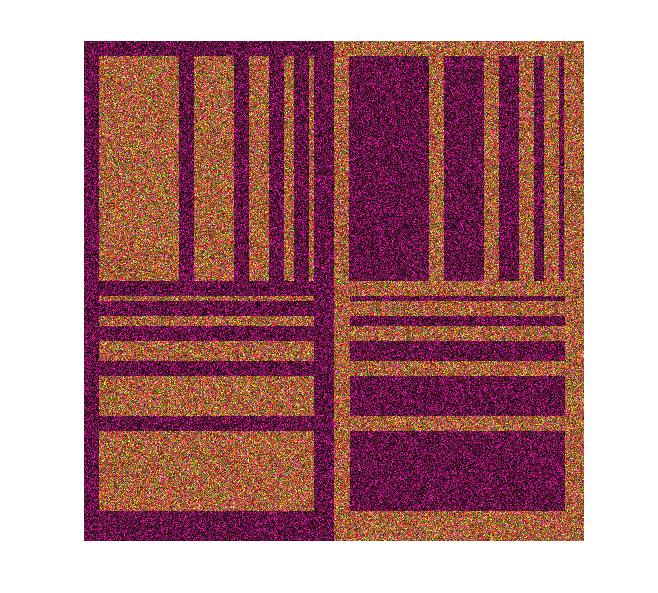
\includegraphics[width=\linewidth]{Eq_Phantom_0p000_1_3_1.jpg}
	\caption{$P_{1,3,0.0}$}\label{fig:awesome_image1}
\endminipage\hfill
\minipage{0.25\textwidth}%
  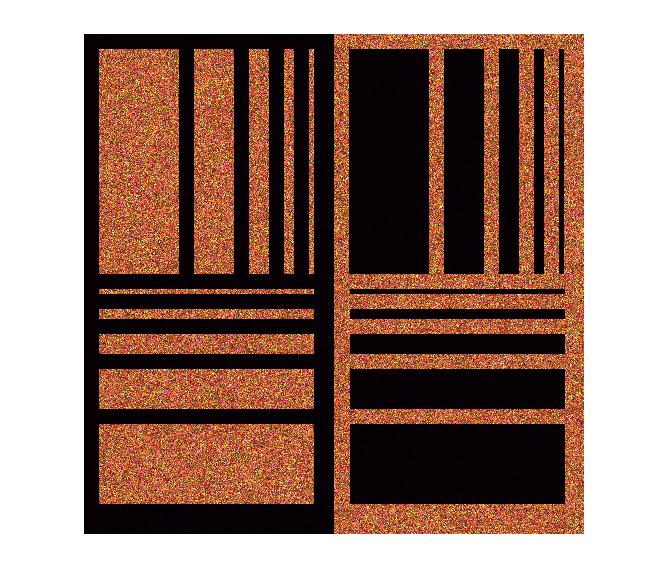
\includegraphics[width=\linewidth]{Eq_Phantom_0p000_1_4_1.jpg}
	\caption{ $P_{1,4,0.0}$}\label{fig:awesome_image1}
\endminipage
\minipage{0.25\textwidth}%
  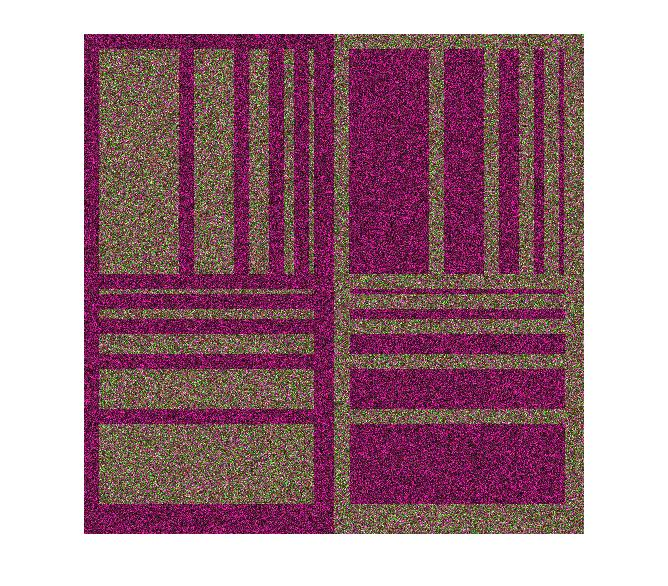
\includegraphics[width=\linewidth]{Eq_Phantom_0p000_1_5_1.jpg}
	\caption{ $P_{1,5,0.0}$}\label{fig:awesome_image1}
\endminipage
%\caption{A really Awesome Image}\label{fig:awesome_image3}
\end{figure}
\begin{figure}[!htb]
\minipage{0.25\textwidth}
  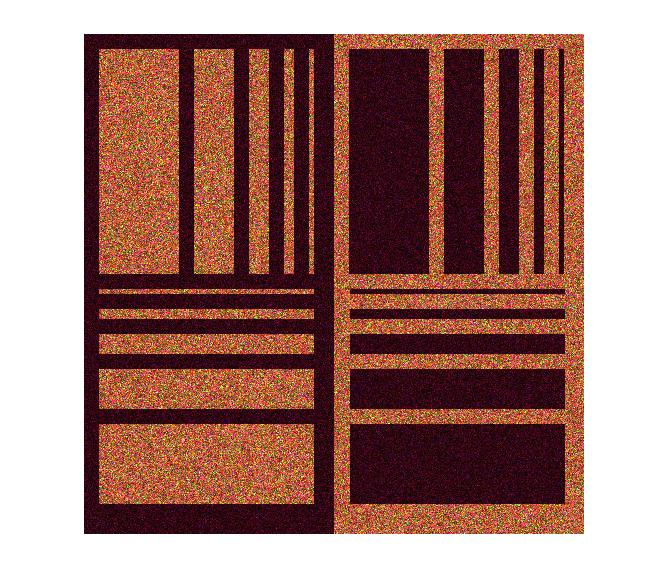
\includegraphics[width=\linewidth]{Eq_Phantom_0p000_2_3_1.jpg}
	\caption{$P_{2,3,0.0}$}\label{fig:awesome_image1}
\endminipage\hfill
\minipage{0.25\textwidth}
  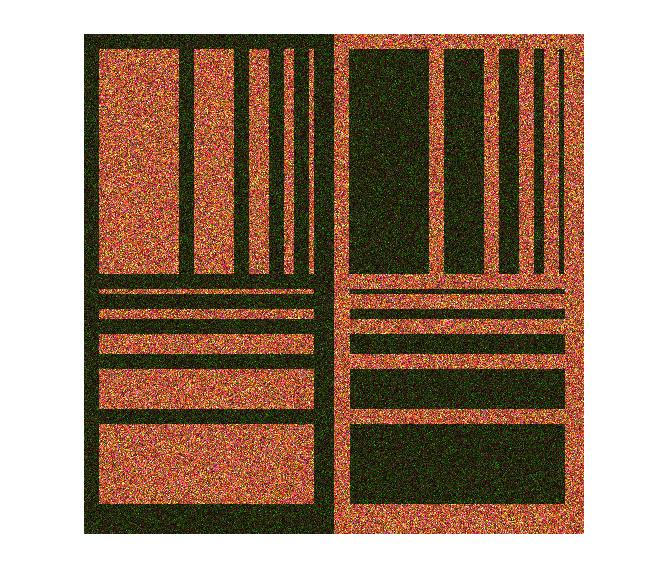
\includegraphics[width=\linewidth]{Eq_Phantom_0p000_2_4_1.jpg}
	\caption{$P_{2,4,0.0}$}\label{fig:awesome_image1}
\endminipage\hfill
\minipage{0.25\textwidth}%
  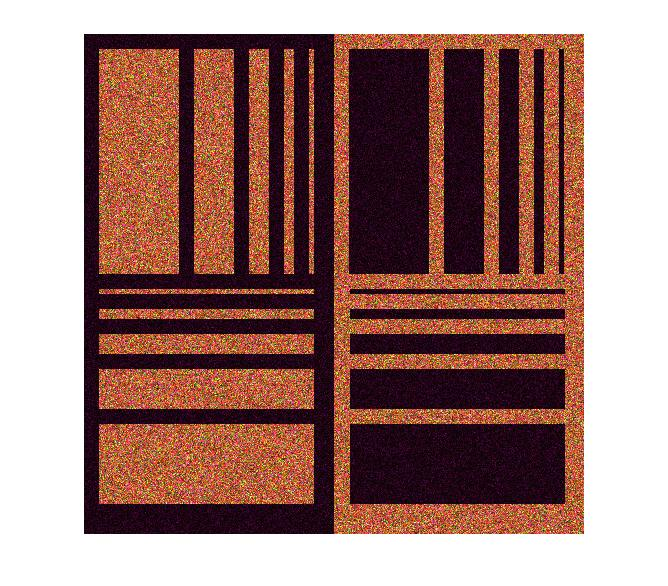
\includegraphics[width=\linewidth]{Eq_Phantom_0p000_2_5_1.jpg}
	\caption{ $P_{2,5,0.0}$}\label{fig:awesome_image1}
\endminipage
\minipage{0.25\textwidth}%
  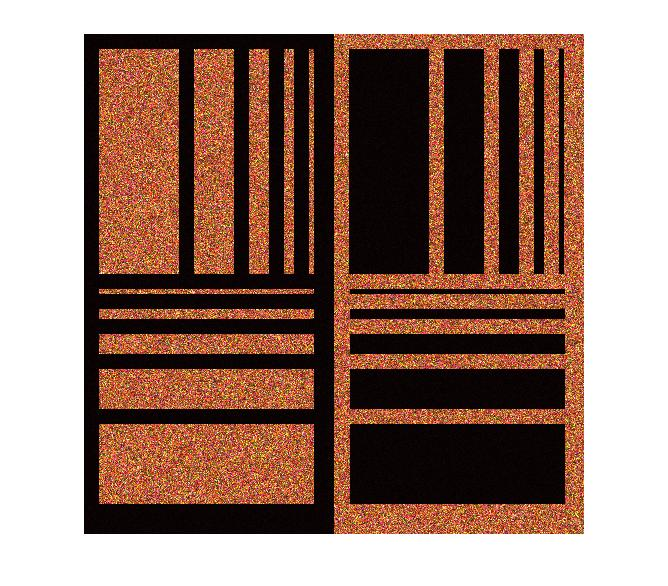
\includegraphics[width=\linewidth]{Eq_Phantom_0p000_3_4_1.jpg}
	\caption{ $P_{3,4,0.0}$}\label{fig:awesome_image1}
\endminipage
%\caption{A really Awesome Image}\label{fig:awesome_image3}
%\end{figure}

%\begin{figure}[!htb]
\minipage{0.25\textwidth}
  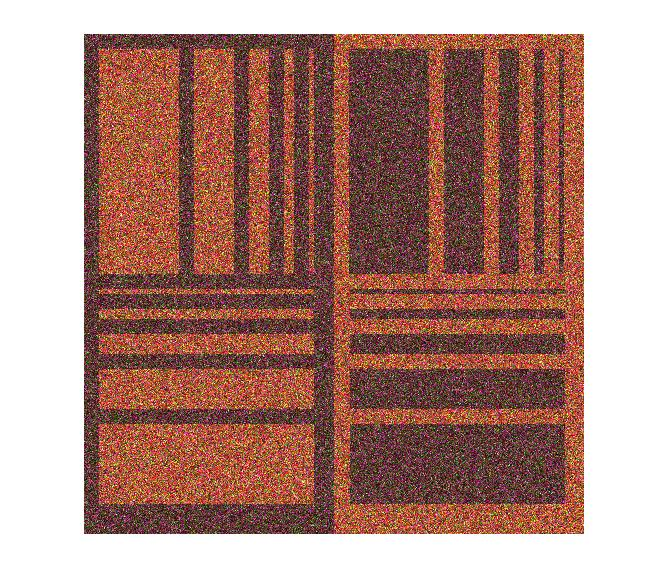
\includegraphics[width=\linewidth]{Eq_Phantom_0p000_3_5_1.jpg}
	\caption{$P_{3,5,0.0}$}\label{fig:awesome_image1}
\endminipage\hfill
\minipage{0.25\textwidth}
  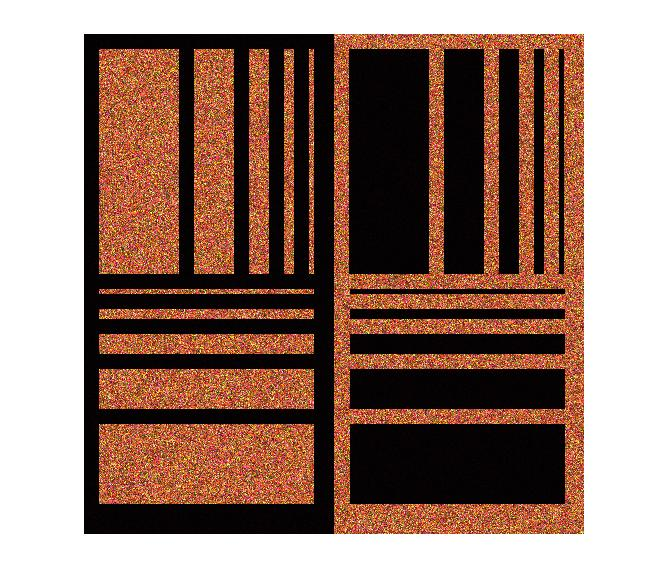
\includegraphics[width=\linewidth]{Eq_Phantom_0p000_4_5_1.jpg}
	\caption{$P_{4,5,0.0}$}\label{fig:awesome_image1}
\endminipage\hfill
%\caption{A really Awesome Image}\label{fig:awesome_image3}
\end{figure}

\subsubsection{Imagens  {\it Phantons} $P_{k_1,k_2,0}$ - Visualização com histeq} 


\textcolor{blue}{São realizadas equalizações das imagens usando o comando histeq(I)}

\textcolor{red}{Para essa imagens está sendo usado o matlab, cuidar ainda algumas discrepância em relação ao artigo}

\begin{figure}[!htb]
\minipage{0.25\textwidth}
  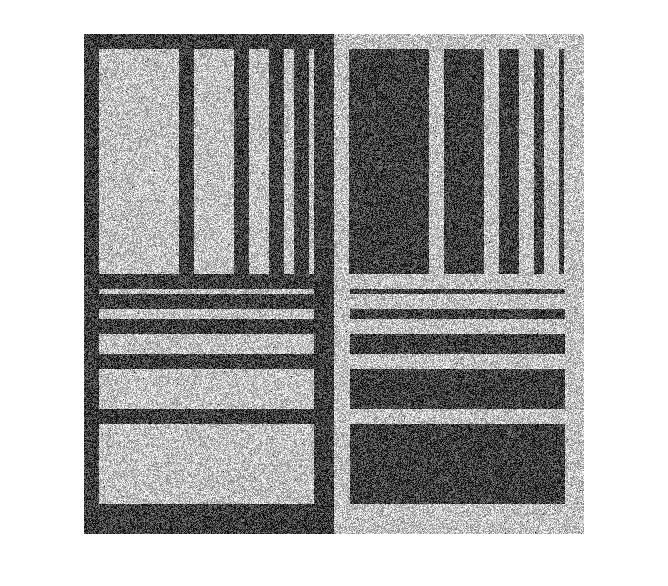
\includegraphics[width=\linewidth]{Eq_Phantom_0p000_1_2_1_histeq.jpg}
	\caption{$P_{1,2,0.0}$}\label{fig:awesome_image1}
\endminipage\hfill
\minipage{0.25\textwidth}
  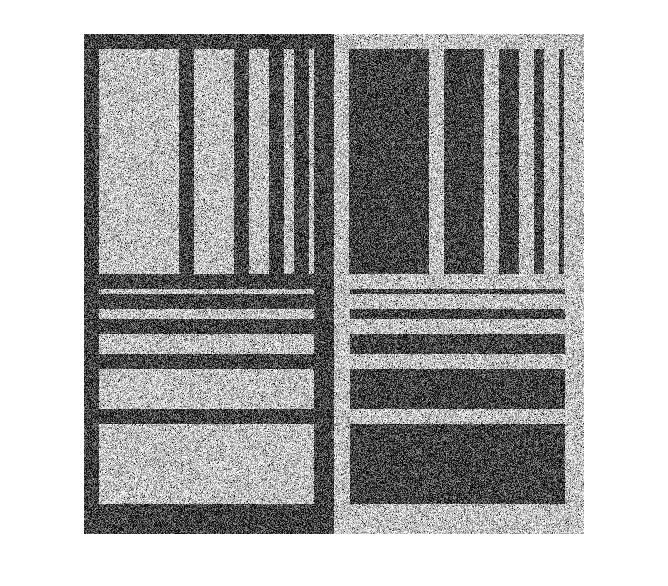
\includegraphics[width=\linewidth]{Eq_Phantom_0p000_1_3_1_histeq.jpg}
	\caption{$P_{1,3,0.0}$}\label{fig:awesome_image1}
\endminipage\hfill
\minipage{0.25\textwidth}%
  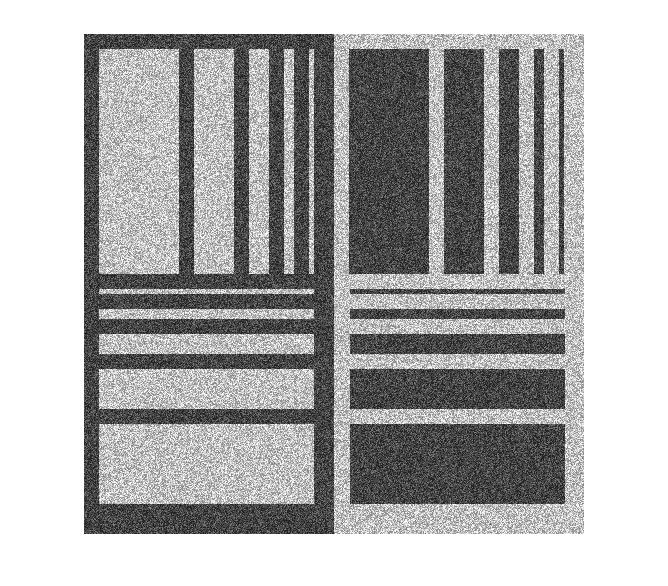
\includegraphics[width=\linewidth]{Eq_Phantom_0p000_1_4_1_histeq.jpg}
	\caption{ $P_{1,4,0.0}$}\label{fig:awesome_image1}
\endminipage
\minipage{0.25\textwidth}%
  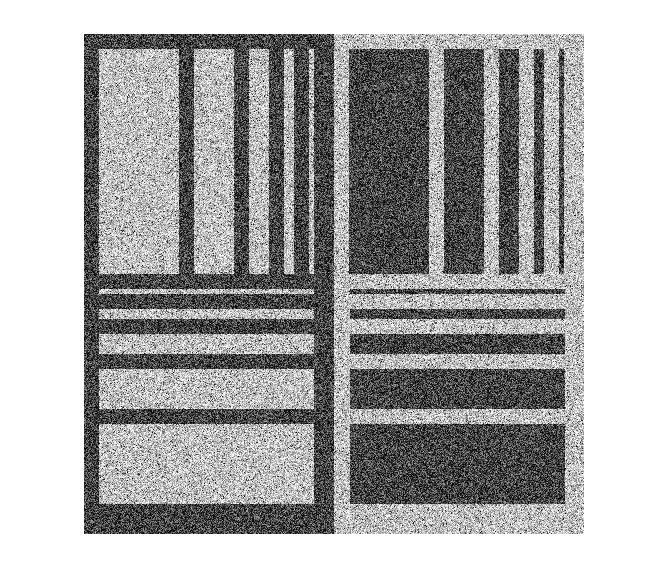
\includegraphics[width=\linewidth]{Eq_Phantom_0p000_1_5_1_histeq.jpg}
	\caption{ $P_{1,5,0.0}$}\label{fig:awesome_image1}
\endminipage
%\caption{A really Awesome Image}\label{fig:awesome_image3}
\end{figure}
\begin{figure}[!htb]
\minipage{0.25\textwidth}
  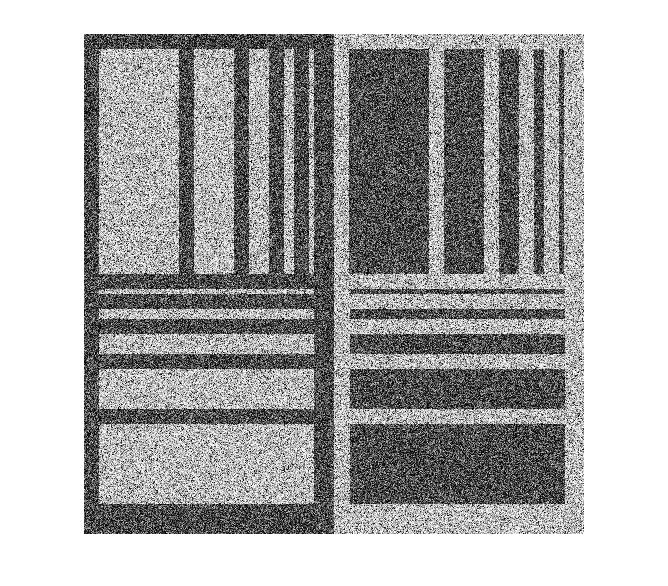
\includegraphics[width=\linewidth]{Eq_Phantom_0p000_2_3_1_histeq.jpg}
	\caption{$P_{2,3,0.0}$}\label{fig:awesome_image1}
\endminipage\hfill
\minipage{0.25\textwidth}
  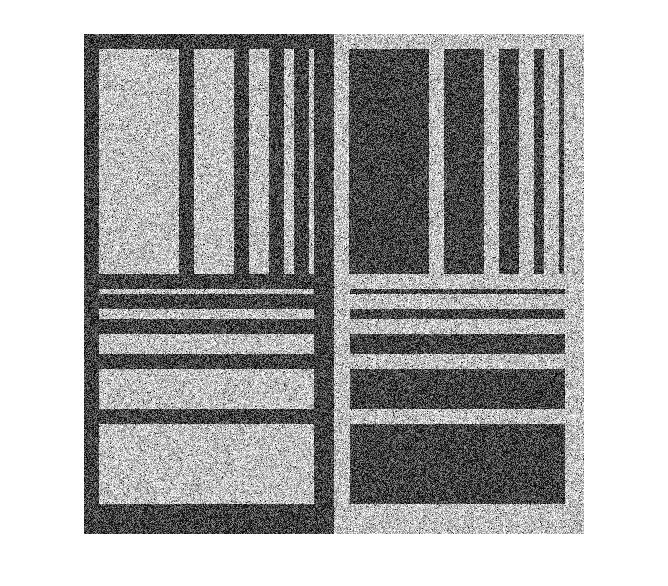
\includegraphics[width=\linewidth]{Eq_Phantom_0p000_2_4_1_histeq.jpg}
	\caption{$P_{2,4,0.0}$}\label{fig:awesome_image1}
\endminipage\hfill
\minipage{0.25\textwidth}%
  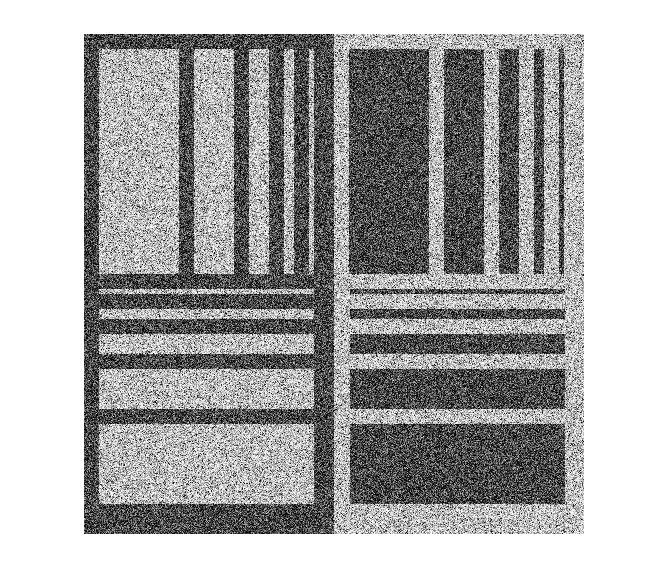
\includegraphics[width=\linewidth]{Eq_Phantom_0p000_2_5_1_histeq.jpg}
	\caption{ $P_{2,5,0.0}$}\label{fig:awesome_image1}
\endminipage
\minipage{0.25\textwidth}%
  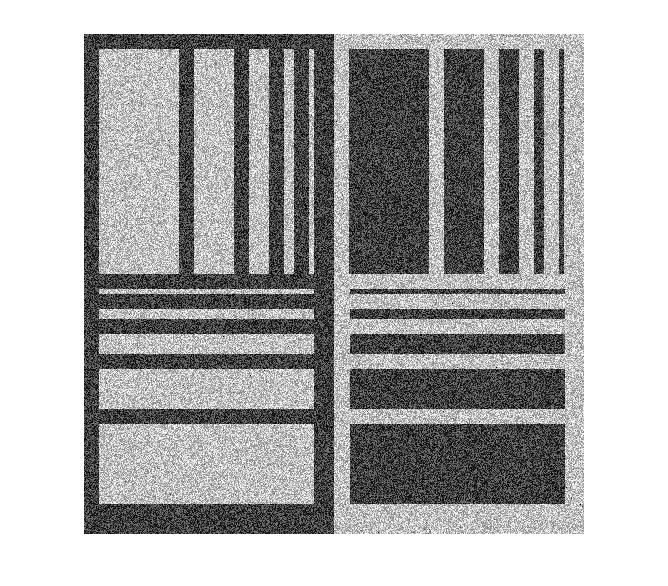
\includegraphics[width=\linewidth]{Eq_Phantom_0p000_3_4_1_histeq.jpg}
	\caption{ $P_{3,4,0.0}$}\label{fig:awesome_image1}
\endminipage
%\caption{A really Awesome Image}\label{fig:awesome_image3}
%\end{figure}

%\begin{figure}[!htb]
\minipage{0.25\textwidth}
  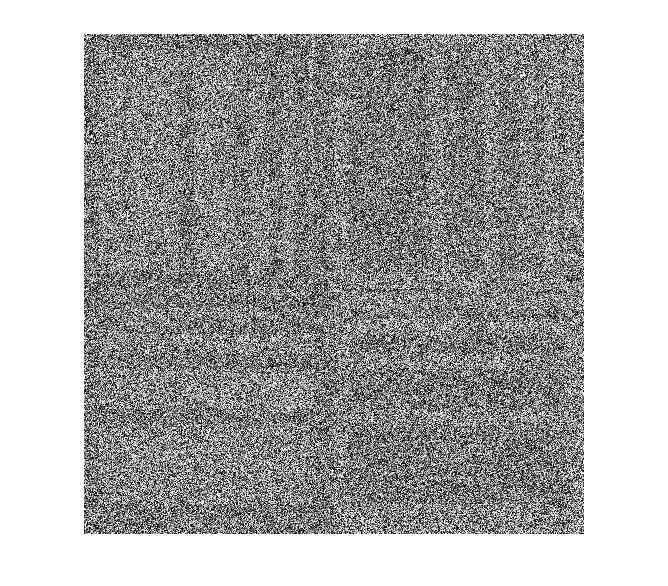
\includegraphics[width=\linewidth]{Eq_Phantom_0p000_3_5_1_histeq.jpg}
	\caption{$P_{3,5,0.0}$}\label{fig:awesome_image1}
\endminipage\hfill
\minipage{0.25\textwidth}
  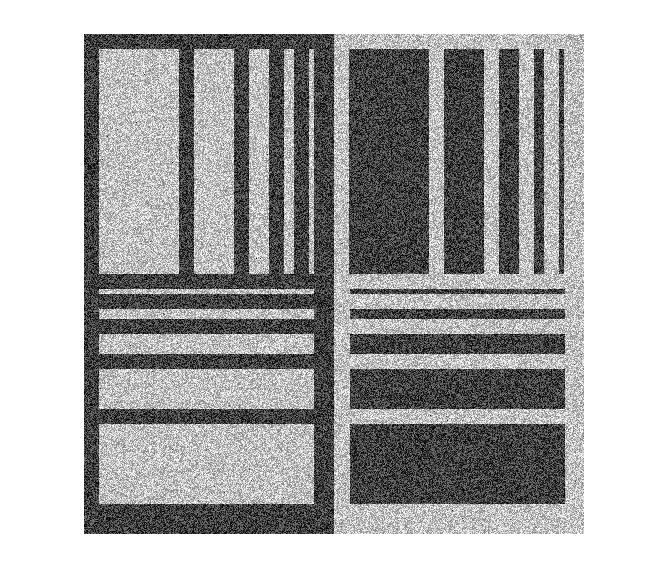
\includegraphics[width=\linewidth]{Eq_Phantom_0p000_4_5_1_histeq.jpg}
	\caption{$P_{4,5,0.0}$}\label{fig:awesome_image1}
\endminipage\hfill
%\caption{A really Awesome Image}\label{fig:awesome_image3}
\end{figure}

\subsection{Estudo do artigo  \cite{nhfc}}

Artigo que discutirá métodos de detecção de borda em imagens Polsar com multiplas visadas. A ideia básica é detectar o ponto de transição em uma faixa tão fina quanto possível entre duas regiões da imagem.

Os métodos clássicos de detecção de bordas assumem que o ruído é aditivo, tornando esses métodos ineficiêntes para aplicação em imagens PolSAR. O ruídos neste tipo de imagens é do tipo {\it speckle} que tem natureza multiplicativa e torna images SAR uma tarefa desafiadora.

Podemos indicar que o problema de detecção de borda pode ser resumido em três importantes aspectos:
\begin{enumerate}
	\item o procedimento para detecção,
	\item a determinação de uma posição mais acurada da posição da borda,
	\item a especificação de tamanho para uma janela (pode ser uma janela quadrada ou ou em uma faixa de dados). 
\end{enumerate}

O tamanho dá janela pode influênciar em alguns aspectos como por exemplo, uma janela pequena pode não conter informações para identificar a presença de bordas, ou janelas maiores podem obter informações para mais de uma borda. Assim o tamanho de janela ideal é aquele que contém as informaões para detecção de uma borda. Vamos assumir que há uma borda na janela fornecida pela seleção inicial.

A proposta do artigo extende este procedimento em três sentidos:
\begin{enumerate}
	\item as mais finas faixas possíveis usadas, inclusive do tamanho de um pixel,
	\item distâncias estocásticas e diferenças de entropias são aplicadas como função objetivo para serem maximizadas, não somente a função de verosimilhança,
	\item A influência da resolução espacial da imagem é usada. 
\end{enumerate}

\subsubsection{Detecção de bordas em imagens PolSAR}

De uma maneira geral, a ideia se baseia em encontrar um ponto de transição em uma faixa de dados o qual é considerado uma estimativa de posicionamento da borda. O estimador é o máximo de uma função dada. 

As metodologias de detecção de bordas nesse artigo ocorrem em diversos estágios:

\begin{enumerate}
	\item identificar o centróide de uma área de interesse de maneira automática, semiautomática ou manual,  
	\item Construindo raios do centróide para fora da área de interesse,
	\item Coletando dados em torno dos raios,
	\item detectar pontos na faixa de dados os quais fornecem evidências de mudanças de propriedades, ou seja, uma transição,
	\item Definindo o contorno usando um método de interpolação entre os pontos de transição, por exemplo as B-Splines.
\end{enumerate}

Inicialmente, escolhemos uma região $\it R$ com centroíde $\bf C$ e traçamos raios iniciando em $\it C$ e indo até um ponto de controle $P_i$, com $i=1,2,\dots, S$, este pontos de controle estão fora da região $\it R$. Teremos $S$ raios resultantes representados por ${\bf s^{(i)}}=\overline{CP_i}$ com ângulos $\epsilon_{i}=\angle ({\bf s_{(i)}},{\bf s_{(i+1)}})$. 

O raio serão convertido sobre pixel usando o algoritmo {\it Bresenham's midpoint line algorithm}, esse algoritmo fornece uma fina representação digital para o raio.

Vamos assumir que os dados seguem uma distribuição complexa Wishart e com sua respectiva função de distribuíção dado por 
\begin{equation}\label{eqn120}
	f_{\mathbf{Z}}(\mathbf{Z^{'}};\mathbf{\Sigma},L)=\frac{L^{mL}|\mathbf{Z^{'}}|^{L-m}}{|\mathbf{\Sigma}|^{L}\Gamma_m(L)} \exp(-L tr(\mathbf{\Sigma}^{-1}\mathbf{Z^{'}})), \\
\end{equation}
onde $\mathbf{Z^{'}}$ é um possível resultado para $\mathbf{Z}$, $\mathbf{\Sigma}$ representa a matriz de covariância, $L$ é o número de visadas, $m$ é o número de canais polarizados.
Sendo ainda, a constante de normalização $\Gamma_m(L)$ é a função Gamma multivariada definida como 
\begin{equation}\label{eqn121}
	\Gamma_m(L)=\pi^{\frac{1}{2}m(m-1)} \prod_{i=0}^{m-1}\Gamma(L-i) \\
\end{equation}
sendo $\Gamma(\cdot)$ a função Gamma e $|\cdot|$, $tr(\cdot)$ são respectivamente o determinande e o traço de uma matriz. Vamoas denotar a distribuíção Wishart como $W(\Sigma,L)$. 

A faixa de dados coletada no {\it i}-ésimo raio {\bf $s^{i}$} , $i=1,2,\dots, S$, contém $N^{(i)}$ pixels. Para cada pixel {\it k} em uma dada faixa {\it i} é assumida que pode ser descrita pelo resultado da matriz $\mathbf{Z_{k}^{(i)}}$ que é um distribuíção de Wishart.  


\begin{equation}\label{eqn122}
 \left\{
\begin{array}{cl}
	Z_{k}^{(i)}\sim W(\Sigma_{A}^{(i),L_{A}^{(i)}}),& \mbox{para}\quad k=1,\dots,j^{(i)}  \\
	Z_{k}^{(i)}\sim W(\Sigma_{B}^{(i),L_{B}^{(i)}}),& \mbox{para}\quad k=j^{(i)} + 1,\dots,N^{(i)}  \\
\end{array}
\right.
\end{equation}

Podemos definir cada faixa composta de dois tipos de amostras, e cada tipo obedeçe uma lei de Wishart complexa com diferentes parametros. Vamos assumir que o número de visadas é constante para todas a faixas.

A ideia principal é encontrar a posição $j^{(i)}$ em uma faixa ao longo do raio ${\bf s^{(i)}}$ dada alguma regra especifíca.

O modelo proposto em (\ref{eqn122}) assume que existe uma transição ocorrendo ao longo da faixa $\bf s^{(i)}$. 

Na continuidade do trabalho será omitido o indíce $(i)$ para focarmos nossa análise em uma única faixa.

\subsubsection{Máxima verosimilhança}

A função de máxima verosimilhança descrita por (\ref{eqn122}) é dada por

\begin{equation*}
	L(j)=\prod_{k=1}^{j}f_{\mathbf{Z}}(\mathbf{Z}_{k}^{'};\mathbf{\Sigma_{A}},L) \prod_{k=j+1}^{N}f_{\mathbf{Z}}(\mathbf{Z}_{k}^{'};\mathbf{\Sigma_{B}},L) \\
\end{equation*}

Usando propriedades de logaritmos natural teremos,


\begin{equation}\label{eqn123}
	l(j)=\ln(L(j))=\sum_{k=1}^{j}\ln\left(f_{\mathbf{Z}}(\mathbf{Z}_{k}^{'};\mathbf{\Sigma_{A}},L)\right)+ \sum_{k=j+1}^{N}\ln\left(f_{\mathbf{Z}}(\mathbf{Z}_{k}^{'};\mathbf{\Sigma_{B}},L)\right) \\
\end{equation}

realizando as manipulações algébricas na função de distribuíção em cada região
\begin{equation*}
\begin{array}{ccc}
	\ln{\left(f_{\mathbf{Z}}(\mathbf{Z}_{k}^{'};\mathbf{\Sigma},L)\right)}&=&\ln{\left(\frac{L^{mL}|\mathbf{Z}_{k}^{'}|^{L-m}}{|\mathbf{\Sigma}|^{L}\Gamma_m(L)} \exp(-L tr(\mathbf{\Sigma}^{-1}\mathbf{Z}_{k}^{'}))\right)}, \\
	\ln{\left(f_{\mathbf{Z}}(\mathbf{Z}_{k}^{'};\mathbf{\Sigma},L)\right)}&=&\ln{\left(\frac{L^{mL}|\mathbf{Z}_{k}^{'}|^{L-m}}{|\mathbf{\Sigma}|^{L}\Gamma_m(L)}\right)}+\ln{\left(\exp(-L tr(\mathbf{\Sigma}^{-1}\mathbf{Z}_{k}^{'}))\right)}, \\
	\ln{\left(f_{\mathbf{Z}}(\mathbf{Z}_{k}^{'};\mathbf{\Sigma},L)\right)}&=&\ln{\left(L^{mL}|\mathbf{Z}_{k}^{'}|^{L-m}\right)}- \ln{\left(|\mathbf{\Sigma}|^{L}\Gamma_m(L)\right)}-L tr(\mathbf{\Sigma}^{-1}\mathbf{Z}_{k}^{'}), \\
	\ln{\left(f_{\mathbf{Z}}(\mathbf{Z}_{k}^{'};\mathbf{\Sigma},L)\right)}&=&\ln{\left(L^{mL}\right)}+\ln{\left(|\mathbf{Z}_{k}^{'}|^{L-m}\right)}- \ln{\left(|\mathbf{\Sigma}|^{L}\right)}-\ln{\left(\Gamma_m(L)\right)}-L tr(\mathbf{\Sigma}^{-1}\mathbf{Z}_{k}^{'}), \\
	\ln{\left(f_{\mathbf{Z}}(\mathbf{Z}_{k}^{'};\mathbf{\Sigma},L)\right)}&=&mL\ln{\left(L\right)}+(L-m)\ln{\left(|\mathbf{Z}_{k}^{'}|\right)}- L\ln{\left(|\mathbf{\Sigma}|\right)}-\ln{\left(\Gamma_m(L)\right)}-L tr(\mathbf{\Sigma}^{-1}\mathbf{Z}_{k}^{'}), \\
\end{array}
\end{equation*}

Substituindo nas duas parcelas da equação (\ref{eqn123}) levando em consideração as duas regiões diferentes teremos
\begin{equation*}
\begin{array}{rcl}
	l(j)&=&\sum_{k=1}^{j}\left[mL\ln{\left(L\right)}+(L-m)\ln{\left(|\mathbf{Z}_{k}^{'}|\right)}- L\ln{\left(|\mathbf{\Sigma_{A}}|\right)}-\ln{\left(\Gamma_m(L)\right)}-L tr(\mathbf{\Sigma_{A}}^{-1}\mathbf{Z}_{k}^{'}))\right], \\
	&+&\sum_{k=j+1}^{N}\left[mL\ln{\left(L\right)}+(L-m)\ln{\left(|\mathbf{Z}_{k}^{'}|\right)}- L\ln{\left(|\mathbf{\Sigma_{B}}|\right)}-\ln{\left(\Gamma_m(L)\right)}-L tr(\mathbf{\Sigma_{B}}^{-1}\mathbf{Z}_{k}^{'})\right], \\
	l(j)&=&\sum_{k=1}^{N}\left[mL\ln{\left(L\right)}-\ln{\left(\Gamma_m(L)\right)}\right]-\sum_{k=1}^{j}\left[ L\ln{\left(|\mathbf{\Sigma_{A}}|\right)}-L tr(\mathbf{\Sigma_{A}}^{-1}\mathbf{Z}_{k}^{'}))\right], \\
	&+&\sum_{k=1}^{N}\left[(L-m)\ln{\left(|\mathbf{Z}_{k}^{'}|\right)}\right]- \sum_{k=j+1}^{N}\left[L\ln{\left(|\mathbf{\Sigma_{B}}|\right)}-L tr(\mathbf{\Sigma_{B}}^{-1}\mathbf{Z}_{k}^{'})\right], \\
	l(j)&=&N\left[mL\ln{\left(L\right)}-\ln{\left(\Gamma_m(L)\right)}\right]-L\left[j\ln{\left(|\mathbf{\Sigma_{A}}|\right)} +\sum_{k=1}^{j}tr(\mathbf{\Sigma_{A}}^{-1}\mathbf{Z}_{k}^{'})\right], \\
	&+&(L-m)\sum_{k=1}^{N}\ln{\left(|\mathbf{Z}_{k}^{'}|\right)}-L\left[(N-j)\ln{\left(|\mathbf{\Sigma_{B}}|\right)}+ \sum_{k=j+1}^{N}tr(\mathbf{\Sigma_{B}}^{-1}\mathbf{Z}_{k}^{'})\right], \\
	l(j)&=&N\left[mL\ln{\left(L\right)}-\ln{\left(\Gamma_m(L)\right)}\right]-L\left[j\ln{\left(|\mathbf{\Sigma_{A}}|\right)} +(N-j)\ln{\left(|\mathbf{\Sigma_{B}}|\right)}\right], \\
	&+&(L-m)\sum_{k=1}^{N}\ln{\left(|\mathbf{Z}_{k}^{'}|\right)}-L\left[\sum_{k=1}^{j}tr(\mathbf{\Sigma_{A}}^{-1}\mathbf{Z}_{k}^{'})+ \sum_{k=j+1}^{N}tr(\mathbf{\Sigma_{B}}^{-1}\mathbf{Z}_{k}^{'})\right], \\
\end{array}
\end{equation*}

Podemos encontrar uma aproximação para $\Sigma$ usando o estimador de máxima verosimilhança denotado por $\widehat{\Sigma}$.
$$
\widehat{\Sigma_{I}}(j) = \left\{
\begin{array}{lc}
	j^{-1}\sum_{k=1}^{j}\mathbf{Z}_{k}  & \mbox{se}\quad I=A,  \\
        (N-j)^{-1}\sum_{k=j+1}^{N}\mathbf{Z}_{k} & \mbox{se}\quad I=B. \\
\end{array}
\right.
$$

Com isso a equação acima pode ser reescrita por

\begin{equation*}
\begin{array}{rcl}
	l(j)&=&N\left[mL\ln{\left(L\right)}-\ln{\left(\Gamma_m(L)\right)}\right]-L\left[j\ln{\left(|\mathbf{\Sigma_{A}}|\right)} +(N-j)\ln{\left(|\mathbf{\Sigma_{B}}|\right)}\right], \\
	&+&(L-m)\sum_{k=1}^{N}\ln{\left(|\mathbf{Z}_{k}^{'}|\right)}-L\left[\sum_{k=1}^{j}tr(\mathbf{\Sigma_{A}}^{-1}\mathbf{Z}_{k}^{'})+ \sum_{k=j+1}^{N}tr(\mathbf{\Sigma_{B}}^{-1}\mathbf{Z}_{k}^{'})\right], \\
	l(j)&=&N\left[mL\ln{\left(L\right)}-\ln{\left(\Gamma_m(L)\right)}\right]-L\left[j\ln{\left(|\mathbf{\Sigma_{A}}|\right)} +(N-j)\ln{\left(|\mathbf{\Sigma_{B}}|\right)}\right], \\
	&+&(L-m)\sum_{k=1}^{N}\ln{\left(|\mathbf{Z}_{k}^{'}|\right)}-L\left[tr\left(\sum_{k=1}^{j}\mathbf{\Sigma_{A}}^{-1}\mathbf{Z}_{k}^{'}\right)+tr\left( \sum_{k=j+1}^{N}\mathbf{\Sigma_{B}}^{-1}\mathbf{Z}_{k}^{'}\right)\right], \\
	l(j)&=&N\left[mL\ln{\left(L\right)}-\ln{\left(\Gamma_m(L)\right)}\right]-L\left[j\ln{\left(|\mathbf{\Sigma_{A}}|\right)} +(N-j)\ln{\left(|\mathbf{\Sigma_{B}}|\right)}\right], \\
	&+&(L-m)\sum_{k=1}^{N}\ln{\left(|\mathbf{Z}_{k}^{'}|\right)}-L\left[tr\left(\mathbf{\Sigma_{A}}^{-1}\sum_{k=1}^{j}\mathbf{Z}_{k}^{'}\right)+tr\left( \mathbf{\Sigma_{B}}^{-1}\sum_{k=j+1}^{N}\mathbf{Z}_{k}^{'}\right)\right], \\
	l(j)&=&N\left[mL\ln{\left(L\right)}-\ln{\left(\Gamma_m(L)\right)}\right]-L\left[j\ln{\left(|\mathbf{\Sigma_{A}}|\right)} +(N-j)\ln{\left(|\mathbf{\Sigma_{B}}|\right)}\right], \\
	&+&(L-m)\sum_{k=1}^{N}\ln{\left(|\mathbf{Z}_{k}^{'}|\right)}-L\left[mj+(N-j)m\right], \\
	l(j)&=&N\left[mL\ln{\left(L\right)}-\ln{\left(\Gamma_m(L)\right)}\right]-L\left[j\ln{\left(|\mathbf{\Sigma_{A}}|\right)} +(N-j)\ln{\left(|\mathbf{\Sigma_{B}}|\right)}\right], \\
	&+&(L-m)\sum_{k=1}^{N}\ln{\left(|\mathbf{Z}_{k}^{'}|\right)}-LNm, \\
	l(j)&=&N\left[-mL(1-\ln{\left(L\right)})-\ln{\left(\Gamma_m(L)\right)}\right]-L\left[j\ln{\left(|\mathbf{\Sigma_{A}}|\right)} +(N-j)\ln{\left(|\mathbf{\Sigma_{B}}|\right)}\right], \\
	&+&(L-m)\sum_{k=1}^{N}\ln{\left(|\mathbf{Z}_{k}^{'}|\right)}, \\
\end{array}
\end{equation*}

Portanto 
\begin{equation}\label{eqn124}
\begin{array}{rcl}
	l(j)&=&N\left[-mL(1-\ln{\left(L\right)})-\ln{\left(\Gamma_m(L)\right)}\right]-L\left[j\ln{\left(|\mathbf{\widehat{\Sigma}}_{A}(j)|\right)} +(N-j)\ln{\left(|\mathbf{\widehat{\Sigma}}_{B}(j)|\right)}\right], \\
	&+&(L-m)\sum_{k=1}^{N}\ln{\left(|\mathbf{Z}_{k}^{'}|\right)}, \\
\end{array}
\end{equation}

O estimador de máxima verosimilhança $\widehat{j}_{ML}$ do índice de localização onde acontece a transição de região é dado por:


\begin{equation}\label{eqn125}
\begin{array}{rcl}
	\widehat{j}_{ML}&=&\text{arg}\max\limits_{j}l(j).  \\
\end{array}
\end{equation}
\textcolor{red}{obs: No artigo não existe o último termo da equação acima, entender o motivo. }
\subsubsection{Gráfico de $l(j)$}

\subsection{Estudo do artigo  \cite{gmbf}}

Imagem com ruído do tipo {\it speckle} pedem ser modeladas por duas amostras randômicas independentes, uma correspondente ao espalhamento $X$ e outra correspondente ao ruído {\it speckle} $Y$. Desta maneira a imagem pode ser representado por $$Z=X \cdot Y.$$

A distribuíção $g^{0}$ é uma atrativa escolha para modelar dados do tipo SAR devido a sua tratabilidade, expresividade e capacidade de recuperar informações detalhadas dos dados. Podemos representar a densidade por
\begin{equation}\label{eqn126}
	f_{g^{0}}(z)=\frac{2L^{L}\mathbf{\Gamma}(L-\alpha)}{\gamma^{\alpha}\mathbf{\Gamma}(-\alpha)\mathbf{\Gamma}(L)}\frac{z^{2L-1}}{(\gamma+z^2L)^{L-\alpha}}, \quad -\alpha,\gamma,z>0,L\geq 1. \\
\end{equation}
sendo $L$ as visadas realizadas para gerar a imagem.

Para dados de amplitude o ruído {\it speckle} $Y$ é modelado como uma distribuíção randômica gamma $\Gamma^{-\frac{1}{2}}(n,n)$. Um modelo geral para o retroespalhamento $X$ considerado é a lei gaussiana inversa generalizada denotada por $N^{-\frac{1}{2}}(\alpha,\lambda,\gamma)$, descrita no artigo \cite{fmcs}.

Para alguns valores particulares dos parametros da distribuíção $N^{-\frac{1}{2}}$, as distribuíções $\Gamma^{\frac{1}{2}}(\alpha,\lambda)$ e $\Gamma^{-\frac{1}{2}}(\alpha,\lambda)$ são obtidas que por sua vez, da surgimento as distribuíções $K$ e $g^{0}$ que modelam $Z$.

\subsubsection{Gráfico da distribuíção $g^{0}$}

O gráfico abaixo simula as distribuíção $g^{0}$ para diferentes paramêtros estatísticos.

\begin{figure}[hbt]
\centering
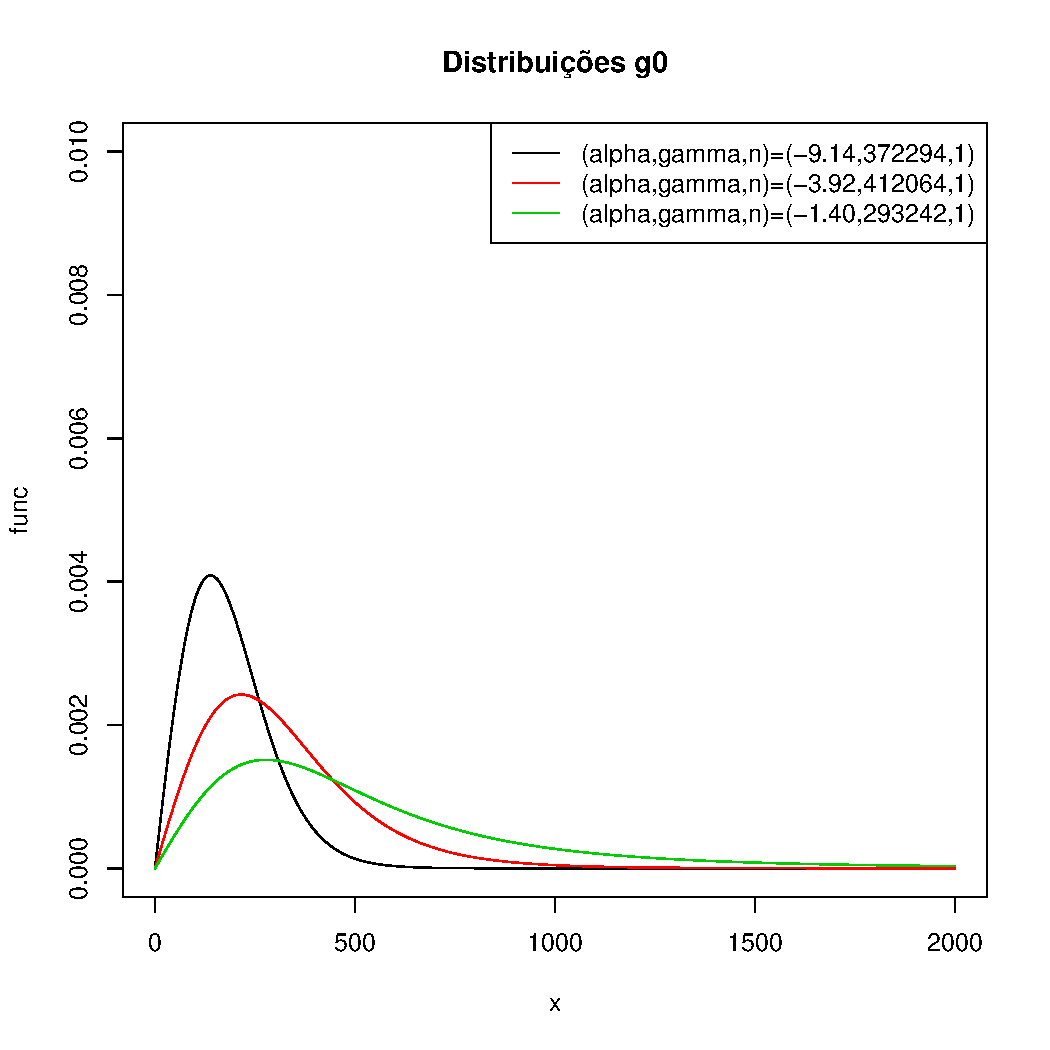
\includegraphics[width=4.0in]{fig_1_gambini_2006.pdf}
	\caption{Distribuíção $g^{0}$.}
\label{fig1}
\end{figure}
\subsubsection{Máxima verosimilhança}

As ideia apresentadas nesta seção são similares com as ideias do artigo \cite{nhfc} e descritos na seção anterior, a mudança está na troca da função de densidade de probabilidades que será usada, nesta seção usaremos a função (\ref{eqn126}).

A função de máxima verosimilhança descrita em duas regiões diferentes analisadas com auxílio de distribuição (\ref{eqn126}) é dada por

\begin{equation*}
	L(j)=\prod_{k=1}^{j}f_{g^{0}}(z_{k}, \alpha_{A}, \gamma_{A} ) \prod_{k=j+1}^{N}f_{g^{0}}(z_{k}, \alpha_{B}, \gamma_{B} ) \\
\end{equation*}

Usando propriedades de logaritmos natural teremos,


\begin{equation}\label{eqn127}
	l(j)=\ln(L(j))=\sum_{k=1}^{j}\ln\left(f_{g^{0}}(z_{k}, \alpha_{A}, \gamma_{A} )\right)+ \sum_{k=j+1}^{N}\ln\left(f_{g^{0}}(z_{k}, \alpha_{B}, \gamma_{B} )\right) \\
\end{equation}

realizando as manipulações algébricas na função de distribuíção em cada região
\begin{equation*}
\begin{array}{ccc}
	\ln{(f_{g^{0}}(z_{k}, \alpha, \gamma))}&=&\ln{\left(\frac{2L^{L}\mathbf{\Gamma}(L-\alpha)}{\gamma^{\alpha}\mathbf{\Gamma}(-\alpha)\mathbf{\Gamma}(L)}\frac{z^{2L-1}}{(\gamma+z^2L)^{L-\alpha}},\right)}, \\
	\ln{(f_{g^{0}}(z_{k}, \alpha, \gamma))}&=&\ln{(2L^{L}\mathbf{\Gamma}(L-\alpha)z^{2L-1})}-\ln{(\gamma^{\alpha}\mathbf{\Gamma}(-\alpha)\mathbf{\Gamma}(L)(\gamma+z^2L)^{L-\alpha})}, \\
	\ln{(f_{g^{0}}(z_{k}, \alpha, \gamma))}&=&\ln{(2)}+\ln{(L^{L})}+\ln{(\mathbf{\Gamma}(L-\alpha))}+\ln{(z^{2L-1})} \\
	    &-&\ln{(\gamma^{\alpha})} -\ln{(\mathbf{\Gamma}(-\alpha))}-\ln{(\mathbf{\Gamma}(L))}-\ln{((\gamma+z^2L)^{L-\alpha})}, \\
	\ln{(f_{g^{0}}(z_{k}, \alpha, \gamma))}&=&\ln{(2)}+L\ln{(L)}+\ln{(\mathbf{\Gamma}(L-\alpha))}+(2L-1)\ln{(z)} \\
	    &-&\alpha\ln{(\gamma)} -\ln{(\mathbf{\Gamma}(-\alpha))}-\ln{(\mathbf{\Gamma}(L))}-(L-\alpha)\ln{(\gamma+z^2L)}, \\
\end{array}
\end{equation*}

Substituindo nas duas parcelas da equação (\ref{eqn127}) levando em consideração as duas regiões diferentes teremos
\begin{equation*}
\begin{array}{rcl}
	l(j)&=&\sum_{k=1}^{j}\left[\ln{(2)}+L\ln{(L)}+\ln{(\mathbf{\Gamma}(L-\alpha_{A}))}+(2L-1)\ln{(z)}\right., \\
	&-&\left.\alpha_{A}\ln{(\gamma_{A})} -\ln{(\mathbf{\Gamma}(-\alpha_{A}))}-\ln{(\mathbf{\Gamma}(L))}-(L-\alpha_{A})\ln{(\gamma_{A}+z^2L)}\right]\\
	&+&\sum_{k=j+1}^{N}\left[ \ln{(2)}+L\ln{(L)}+\ln{(\mathbf{\Gamma}(L-\alpha_{B}))}+(2L-1)\ln{(z)}\right. \\
	&-&\left.\alpha_{B}\ln{(\gamma_{B})} -\ln{(\mathbf{\Gamma}(-\alpha_{B}))}-\ln{(\mathbf{\Gamma}(L))}-(L-\alpha_{B})\ln{(\gamma_{B}+z^2L)}\right]\\
	l(j)&=&\sum_{k=1}^{j}\left[\ln{(2)}+L\ln{(L)}-\ln{\Gamma(L)}\right]+(2L-1)\sum_{k=1}^{N}\ln{(z)} \\
	&+&\sum_{k=1}^{j}\left[\ln{(\Gamma(L-\alpha_{A}))}-\alpha_{A}\ln{(\gamma_{A})} -\ln{(\mathbf{\Gamma}(-\alpha_{A}))}-(L-\alpha_{A})\ln{(\gamma_{A}+z^2L)}\right]\\
	&+&\sum_{k=j+1}^{N}\left[\ln{(2)}+L\ln{(L)}-\ln{\Gamma(L)}\right] \\
	&+&\sum_{k=j+1}^{N}\left[\ln{(\mathbf{\Gamma}(L-\alpha_{B}))}-\alpha_{B}\ln{(\gamma_{B})} -\ln{(\mathbf{\Gamma}(-\alpha_{B}))}-(L-\alpha_{B})\ln{(\gamma_{B}+z^2L)}\right]\\
	l(j)&=&\left[\ln{(2)}+L\ln{(L)}-\ln{\Gamma(L)}\right]j+(2L-1)\sum_{k=1}^{N}\ln{(z)} \\
	&+&\left[\ln{(\Gamma(L-\alpha_{A}))}-\alpha_{A}\ln{(\gamma_{A})} -\ln{(\mathbf{\Gamma}(-\alpha_{A}))}\right]j\\
	  &+&\left[\ln{(2)}+L\ln{(L)}-\ln{\Gamma(L)}\right](N-j) \\
	&+&\left[\ln{(\mathbf{\Gamma}(L-\alpha_{B}))}-\alpha_{B}\ln{(\gamma_{B})} -\ln{(\mathbf{\Gamma}(-\alpha_{B}))}\right](N-j) \\
	&-&(L-\alpha_{B})\sum_{k=j+1}^{N}\ln{(\gamma_{B}+z^2L)}-(L-\alpha_{A})\sum_{k=1}^{j}\ln{(\gamma_{A}+z^2L)}\\
	l(j)&=&\left[\ln{(2)}+L\ln{(L)}-\ln{\Gamma(L)}\right]N+(2L-1)\sum_{k=1}^{N}\ln{(z)} \\
	&+&\left[\ln{(\Gamma(L-\alpha_{A}))}-\alpha_{A}\ln{(\gamma_{A})} -\ln{(\mathbf{\Gamma}(-\alpha_{A}))}\right]j\\
	&+&\left[\ln{(\mathbf{\Gamma}(L-\alpha_{B}))}-\alpha_{B}\ln{(\gamma_{B})} -\ln{(\mathbf{\Gamma}(-\alpha_{B}))}\right](N-j) \\
	&-&(L-\alpha_{B})\sum_{k=j+1}^{N}\ln{(\gamma_{B}+z^2L)}-(L-\alpha_{A})\sum_{k=1}^{j}\ln{(\gamma_{A}+z^2L)}\\
\end{array}
\end{equation*}

Por facilidade de notação podemos definir as seguintes notações
$$
\begin{array}{lcl}
	k_1&=& \left[\ln{(2)}+L\ln{(L)}-\ln{\Gamma(L)}\right]\\
	k_2&=& \ln{(\Gamma(L-\alpha_{A}))}-\alpha_{A}\ln{(\gamma_{A})} -\ln{(\mathbf{\Gamma}(-\alpha_{A}))}\\
	k_3&=& \ln{(\mathbf{\Gamma}(L-\alpha_{B}))}-\alpha_{B}\ln{(\gamma_{B})} -\ln{(\mathbf{\Gamma}(-\alpha_{B}))}\\
\end{array}
$$

Com isso a equação acima pode ser reescrita por
\begin{equation*}
\begin{array}{rcl}
	l(j)&=&k_1N+(2L-1)\sum_{k=1}^{N}\ln{(z)} +k_2j+k_3(N-j) \\
	&-&(L-\alpha_{B})\sum_{k=j+1}^{N}\ln{(\gamma_{B}+z^2L)}-(L-\alpha_{A})\sum_{k=1}^{j}\ln{(\gamma_{A}+z^2L)}\\
	l(j)&=&k_1N+(2L-1)\sum_{k=1}^{N}\ln{(z)} +k_2j+k_3N-k_3j \\
	&-&(L-\alpha_{B})\sum_{k=j+1}^{N}\ln{(\gamma_{B}+z^2L)}-(L-\alpha_{A})\sum_{k=1}^{j}\ln{(\gamma_{A}+z^2L)}\\
        l(j)&=&\left((k_1+k_3)N+(2L-1)\sum_{k=1}^{N}\ln{(z)}\right) +(k_2-k_3)j \\
	&-&(L-\alpha_{B})\sum_{k=j+1}^{N}\ln{(\gamma_{B}+z^2L)}-(L-\alpha_{A})\sum_{k=1}^{j}\ln{(\gamma_{A}+z^2L)}\\
\end{array}
\end{equation*}

Novamente por facilidade de notação podemos definir as seguintes notações
$$
\begin{array}{lcl}
    \bar{k}_1&=&(k_1+k_3)N+(2L-1)\sum_{k=1}^{N}\ln{(z)} \\
	\bar{k}_2&=& (k_2-k_3)\\
\end{array}
$$

Com isso a equação acima pode ser reescrita por
\begin{equation}\label{eqn128}
\begin{array}{rcl}
	l(j)&=&\bar{k}_1 +\bar{k}_2j \\
	&-&(L-\alpha_{B})\sum_{k=j+1}^{N}\ln{(\gamma_{B}+z^2L)}-(L-\alpha_{A})\sum_{k=1}^{j}\ln{(\gamma_{A}+z^2L)}\\
\end{array}
\end{equation}

O estimador de máxima verosimilhança $\widehat{j}_{ML}$ do índice de localização onde acontece a transição de região é dado por:

\begin{equation}\label{eqn129}
\begin{array}{rcl}
	\widehat{j}_{ML}&=&\text{arg}\max\limits_{j}l(j).  \\
\end{array}
\end{equation}

\subsubsection{Implementação da equação (\ref{eqn127})}


Nesta seção, será realizado o processo de maximização da função objetivo $l(j)$ conforme a equação (\ref{eqn129}) usando a definição de $l(j)$ como a equação (\ref{eqn127}). Para os testes escolhemos os parametros $(\alpha_r, \gamma_r)=(-9.14, 372294)$ e $(\alpha_b,\gamma_b)=(-3.92,293242)$ que representam os parâmetros estatísticos para a região de interesse da imagem e o seu fundo respectivamente. A figura abaixo mostra o gráfico de $L(j)$ para esses parâmetros.  

\begin{figure}[hbt]
\centering
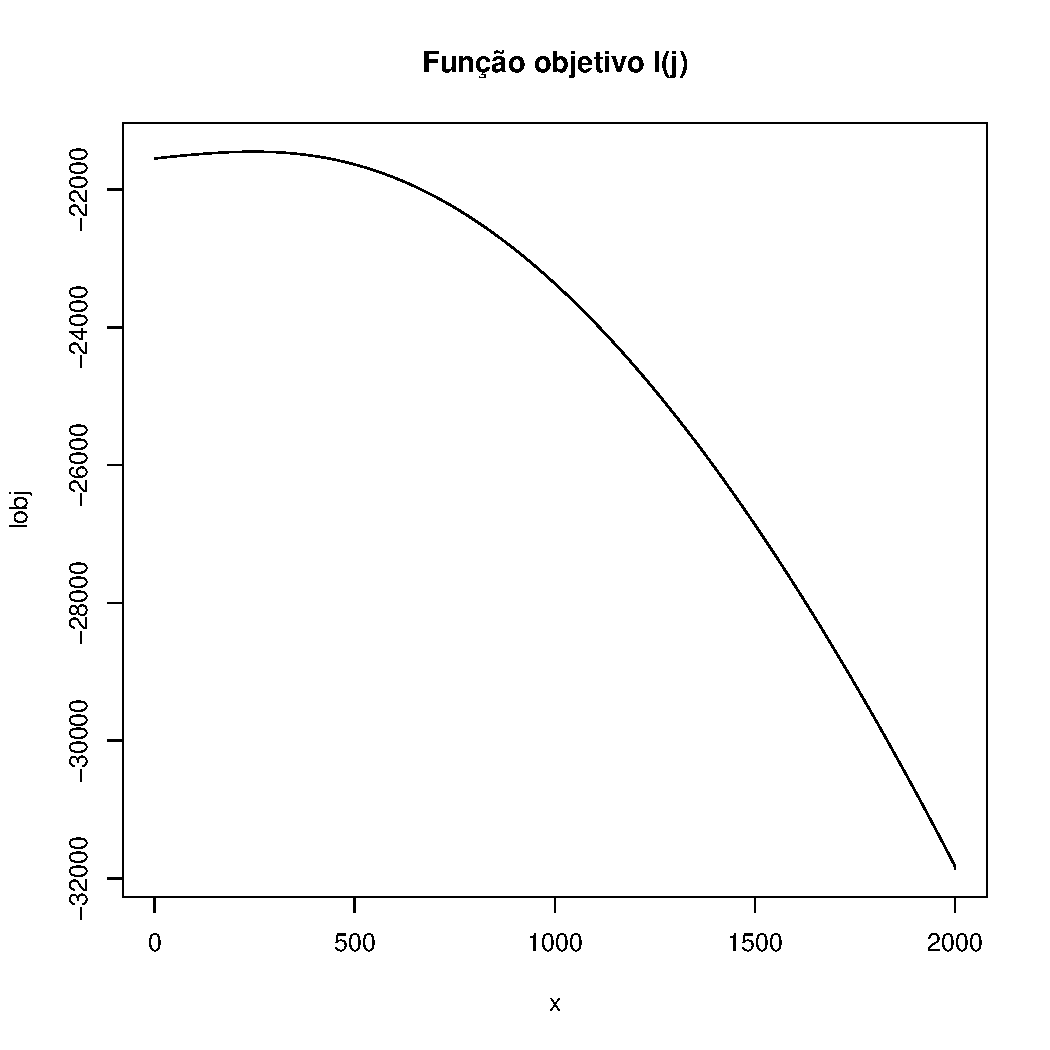
\includegraphics[width=4.0in]{fig_2_gambini_2006_func_objetivo_eq12.pdf}
	\caption{Função objetivo $l(j) -  eq127$.}
\label{fig1}
\end{figure}

O problema de máximizar a função objetivo foi realizada na linguagem de programação R com auxílio da biblioteca {\it maxLik} a qual podemos descrever brevemente como uma ferramente para estimar a máxima verosimilhança com otimização não linear podendo facilmente usar diferentes métodos de otimização. Para mais detalhes podemos consultar \cite{ht}.


\textcolor{red}{O programa está no meu computador pessoal no endereço}

\textcolor{red}{aborba/MEGAsync/mack/alejandro/gitufalmack/doclatex/}

Para iniciar o processo de otimização foi dado um chute inicial $x_0=200\in[0,2000]$ e uma tolerância de $tol=10^{-8}$ para iterações sucessivas como critério de parada do método. Foi usado o método de otimização BFGS.

Os resultados foram compatíveis com o esperado pelo gráfico acima, isto é, o método mostrou como saída $10$ iterações, o valor de abscissa máxima $x_{max}\in[240,250]$ e $-21438.650158$ para a ordenada do valor máximo estimado pelo algoritmo para a função objetivo.

\textcolor{red}{Realizei alguns teste com a variação de tolerância e constatei que os resultados permaneciam os mesmo, pensar sobre isso (precisão simples do programa?)}

\subsubsection{Implementação da equação (\ref{eqn128})}

Nesta seção, será realizado o processo de maximização da função objetivo $l(j)$ conforme a equação (\ref{eqn129}) usando a equação (\ref{eqn128}). Para os testes escolhemos os parametros $(\alpha_r, \gamma_r)=(-9.14, 372294)$ e $(\alpha_b,\gamma_b)=(-3.92,293242)$ que representam os parâmetros estatísticos para a região de interesse da imagem e o seu fundo respectivamente. A figura abaixo mostra o gráfico de $l(j)$ para esses parâmetros.  

\begin{figure}[hbt]
\centering
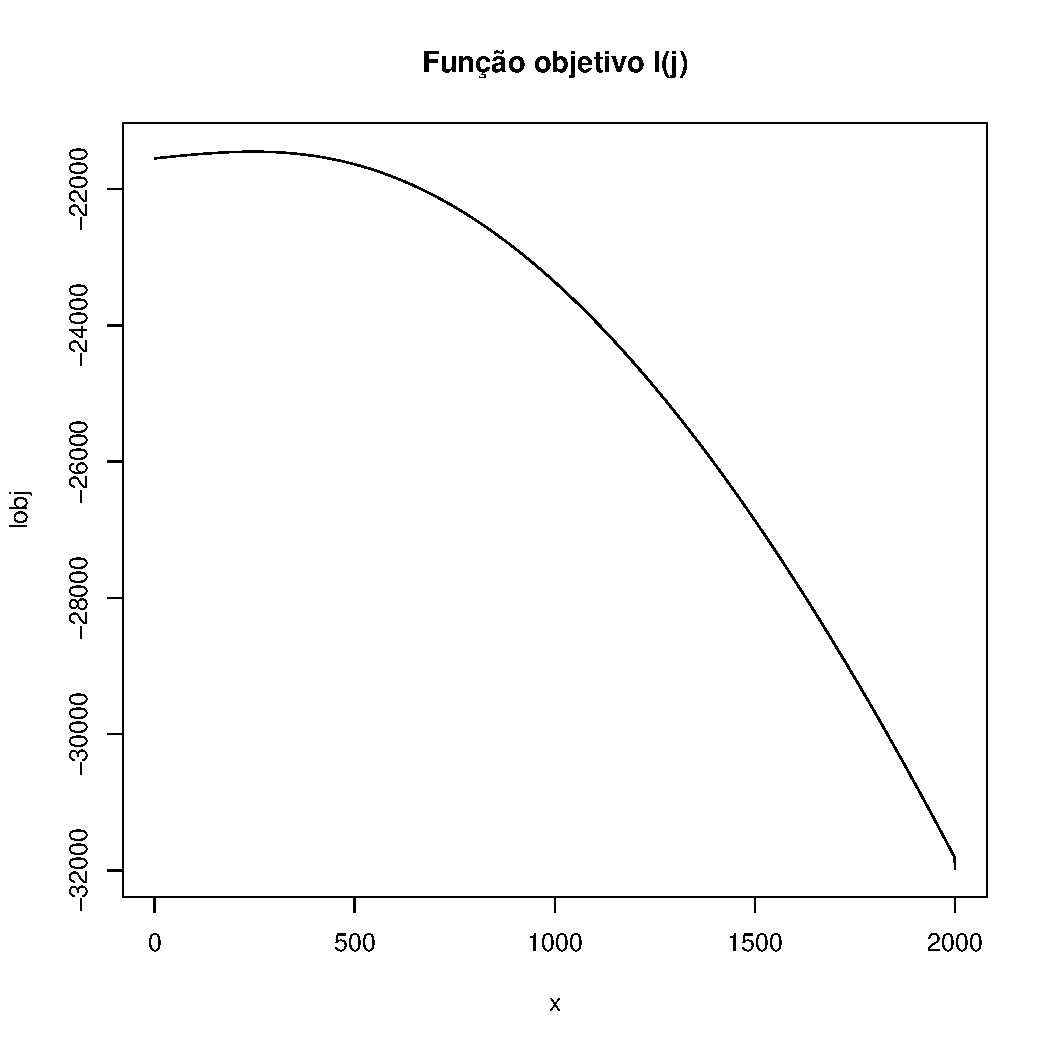
\includegraphics[width=4.0in]{func_objetivo_eq128.pdf}
	\caption{Função objetivo $L(j) - eq128$.}
\label{fig1}
\end{figure}

Podemos observar que a função é mesma pois a equção (\ref{eqn128}) foi deduzida da equação (\ref{eqn127}). A forma da função  objetivo mostrada na figura (\ref{eqn128}) apresenta a vantagem de necessitar uma menor quantidade de conta por iteração ajudando a diminuir o custo computacional.


Para rodar o programa que encontra o estimador de máxima verosimilhança apresentado na equação (\ref{eqn129}) utilizando a função objetivo (\ref{eqn128}) utilizamos o mesmo procedimento da seção anterior

Para iniciar o processo de otimização foi dado um chute inicial $x_0=200\in[0,2000]$ e uma tolerância de $tol=10^{-8}$ para iterações sucessivas como critério de parada do método. Foi usado o método de otimização BFGS.

Os resultados foram compatíveis com o esperado pelo gráfico acima, isto é, o método mostrou como saída $14$ iterações, o valor de abscissa máxima $x_{max}\in[240,260]$ e $-21323.677236$ para a ordenada do valor máximo estimado pelo algoritmo para a função objetivo.

\textcolor{red}{O resultado da otimização foi sensivelmente diferente do anterior, devo fazer uma validação mais consistente desses algoritmos}


\section{Ruído do tipo {\it Speckle} - Texto que estava na tese e eu tirei para a qualificação e um backup para não perder nada}

Nesta seção é apresentado características do ruído {\it Speckle} baseado nas referências \cite{lee}, \cite{lp} e \cite{fmcs}.

Os ruídos do tipo {\it Speckle} são associados a imagens de radar com abetura sintética  devido as ondas de interferência coerênte refletidas de diversos elementos espalhadores da cena alvo. Por exemplo, imagens obtidas por microondas, laser, ultrasonografia, etc. Isto é, os ruídos do tipo {\it Speckle} apareçem devido a fenomênos de interferência entre o sinal eletromagnético  incidente e o sinal refletido. Este tipo de ruído pode tornar a tarefa de interpretar e analisar as imagens tanto visual como automática difícil, reduzindo a efetividade da segmentação detecção de bordas e classificação de caracterísiticas. 

Portanto o entendimento de ruído do tipo {\it Speckle} é essencial para a extração de informação e construção de um algoritmo eficiênte na filtragem do ruído {\it Speckle} para estimar parâmetros geofísicos com intuito de observar nas imagens informaçãos adequadas com a aplicação que necessitamos.

\subsection{A formação do ruído tipo {\it Speckle}}

O radar trabalha focando uma região de interesse que pode ser rugosa, assim o sinal que retorna terá efeito na reflexão de vários alvos espalhadores de sina da região de interesse. Podemos afirmar que as distâncias entre a localização dos alvos espalhadores e o radar variam de maneira randômica. Portanto, a distância entre os alvos espalhadores e o radar é randômica. Podemos afirmar que as ondas recebidas são coerentes na frequência porém não são na fase. Assim, um sinal forte recebido é o somatório de ondas construtivas(em fase) e o sinal fraco é o somatório de ondas destrutivas (fora de fase).

A onda única pode ser representada por $\phi_i=x_i+jy_i$ com $i=1,\dots,M$, então o somatório de ondas podem ser escritos como 

\begin{equation}\label{cap_acf_12}
\begin{array}{ccc}
	\sum_{i=1}^{M}\phi_i&=&\sum_{i=1}^{M}(x_i+jy_i), \\
\end{array}
\end{equation}
\begin{equation}\label{cap_acf_13}
\begin{array}{ccc}
	\sum_{i=1}^{M}(x_i+jy_i)&=&\sum_{i=1}^{M}x_i+j\sum_{i=1}^{M}y_i, \\
\end{array}
\end{equation}
\begin{equation}\label{cap_acf_14}
\begin{array}{ccc}
	\sum_{i=1}^{M}x_i+j\sum_{i=1}^{M}y_i&=&\bar{x}+j\bar{y}=\bar{\phi}, \\
\end{array}
\end{equation}
onde, $\bar{x}=\sum_{i=1}^{M}x_i$ e $\bar{y}=\sum_{i=1}^{M}y_i$ e ainda $\phi$ é a o sinal recebido do $i-$ésimo alvo de espalhamento e $\bar{\phi}$ é a soma de todos os alvos de espalhamento, completando com o número complexo $j$.

A imagem SAR é formada por processamento coerênte formado por sucessivos pulsos. Este processo causa uma variação na itensudade pixel a pixel manifestando assim um padrão granular na imagem, este padrão é chamado de {\it Speckle}. Esse padrão torna a observação da imagem complicada prejudicando sua análise.




\subsubsection{O modelo multiplicativo e o ruído {\it speckle}}


O modelo multiplicativo é uma ferramenta usada para explicar o comportamento estatístico de dados obtidos com coerentes iluminação. Assumindo que a observação com estas imagens são o resultado do produto de duas independentes variáveis randômicas, uma $(X)$ modelando o retroespalhamento do terreno, e outra $(Y)$ modelando o ruído {\it speckle}. O primeiro é considerado real e positivo, enquanto o segundo pode ser complexo.

O valor observado é resultado da variável randômica definida como $Z=X\cdot Y$. Serão definidos os seguintes subescritos $C$, $I$, e $A$ para a referência a complexos, intensidade e amplitude respectivamente.

{\it Speckle} complexo tem distribuição normal bivariada com componentes distribuída identicamente independente tendo média $0$ e variância $\frac{1}{2}$. Assim, $\mathbf{Y}_{C}=(Y_{\mathbb{R}}, Y_{\mathbb{I}})\sim N2(0,\frac{1}{2})$ denota a distribuíção do par.

{\it Multilook intensity speackle} surge tomando a média sobre $n$ amostras independentes de $Y_{I}=\|Y_{C}\|^2$ na qual implica a distribuição gamma denotada por $Y_{I}\sim \Gamma(n,n)$ e caracterizado pela densidade mostrada na figura (\ref{fig9})

\begin{equation}\label{eqn102}
	f_{Y_{I}}(y)=\frac{n^{n}}{\Gamma(n)}y^{n-1}\exp\left(-ny\right),\quad y,n>0 
\end{equation}

\begin{figure}[!htb]
\centering
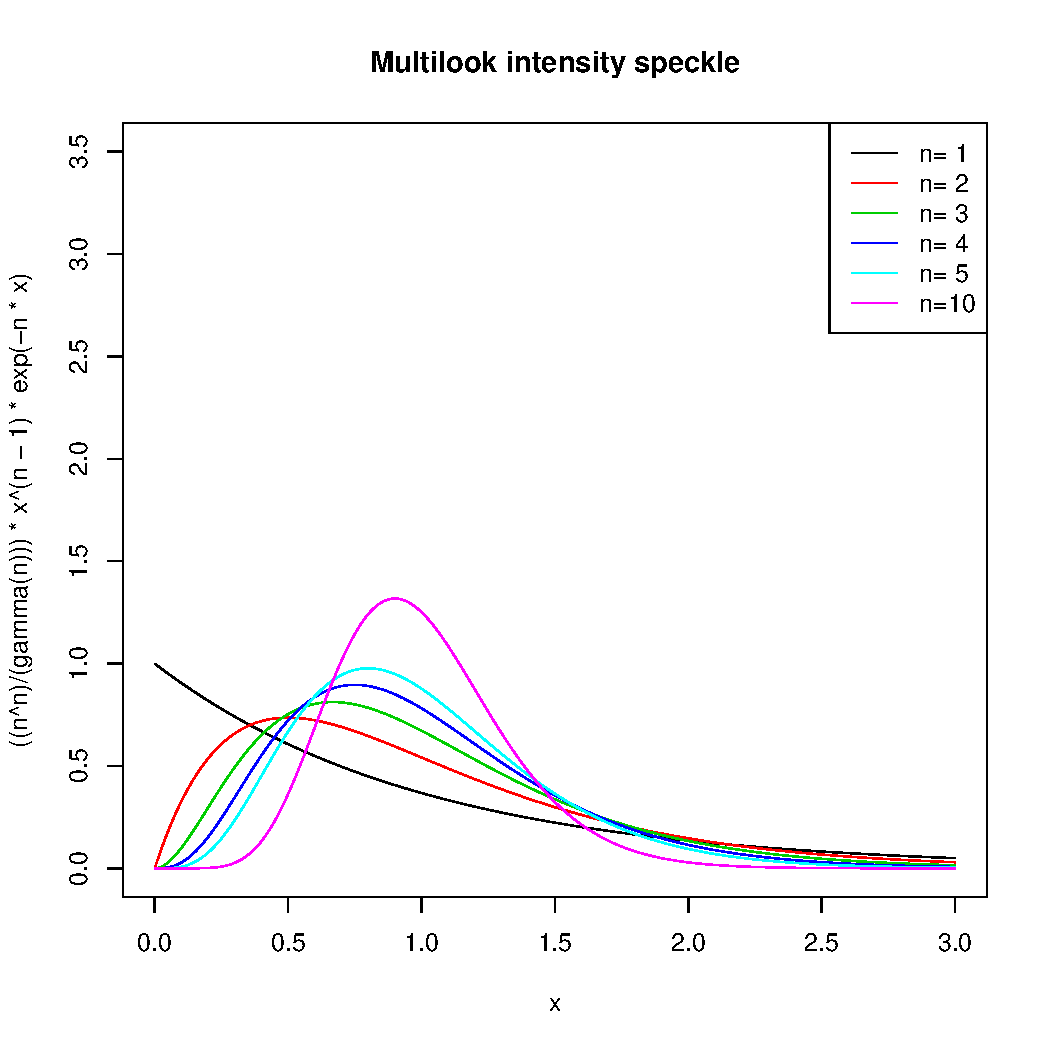
\includegraphics[width=4.0in]{fig_eq_fyi_frery_muller_1997.pdf}
	\caption{Multilook Intensity speckle  para $n\in(1,2,3,4,5,10)$.}
\label{fig9}
\end{figure}

{\it Multilook amplitude speackle} surge tomando a raíz quadrada do {\it Multilook intensity speackle} e portanto a raíz quadrada da distribuíção gamma, denotado por $Y_{A}\sim \Gamma^{\frac{1}{2}}(n,n)$ e caracterizado pela densidade e mostrada na figura  (\ref{fig10}).

\begin{equation}\label{eqn103}
	f_{Y_{A}}(y)=\frac{2n^{n}}{\Gamma(n)}y^{2*n-1}\exp\left(-ny^2\right),\quad y,n>0 
\end{equation}
\begin{figure}[!htb]
\centering
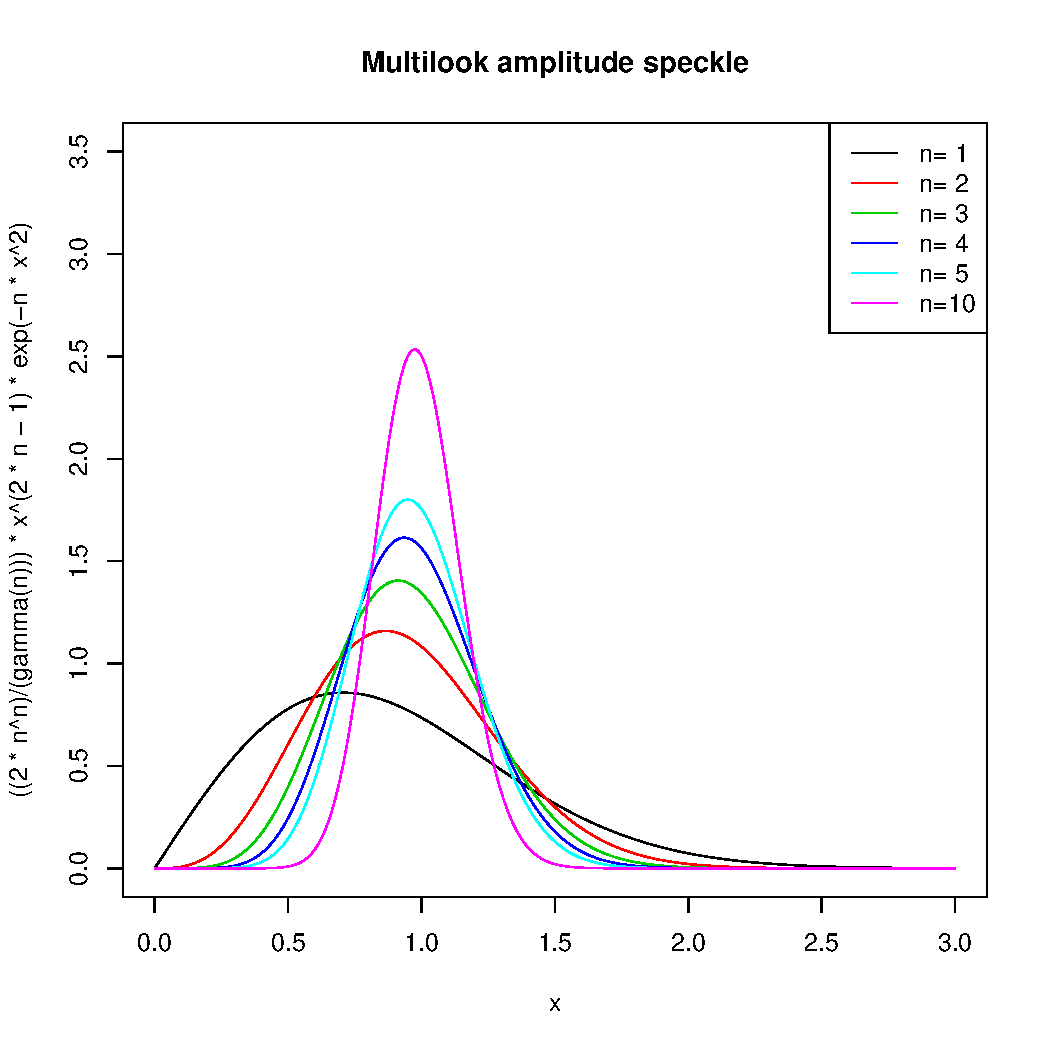
\includegraphics[width=4.0in]{fig_eq_fya_frery_muller_1997.pdf}
	\caption{Multilook Amplitude speckle  para $n\in(1,2,3,4,5,10)$.}
\label{fig10}
\end{figure}
\subsubsection{Amplitude do retroespalhamento}

A amplitude do retroespalhamento obedeçe a raíz quadrada da lei gaussiana inversa generalizada, donotado aqui por $\mathbf{X}_{A}\sim N^{-\frac{1}{2}}(\alpha,\gamma,\lambda)$, sendo sua densidade dada por
\begin{equation}\label{eqn104}
	f_{X_{A}}(x)=\frac{\left(\frac{\lambda}{\gamma}\right)^{\frac{\alpha}{2}}}{K_{\alpha}(2\sqrt{\lambda\gamma})}x^{2\alpha-1}\exp\left(-\frac{\gamma}{x^2}-\lambda x^2\right) 
\end{equation}

Dois casos particulares desta distribuíção são de interesse na análise de dados $SAR$, a raíz quadrada de gamma e a recíproca da raíz quadrada da distribuição gamma. 

A raíz quadrada da distribuição gamma surge quando $\gamma \rightarrow 0$ enquanto $\alpha,\lambda>0$. Esta distribuição é denota aqui por $\Gamma^{\frac{1}{2}}(\alpha,\lambda)$ e caracterizada pela densidade 
\begin{equation}\label{eqn105}
	f_{X_{A}}(x)=\frac{2\lambda^{\alpha}}{\Gamma(\alpha)}x^{2\alpha-1}exp(-\lambda x^2), \quad \alpha,\lambda, x>0. 
\end{equation}
A recíproca da raíz quadrada da distribuição gamma surge quando $\lambda\rightarrow 0$ enquanto $-\alpha,\gamma>0$. Esta distribuição é denotada aqui por $\Gamma^{-\frac{1}{2}}(\alpha,\gamma) $ e caracterizada pela densidade
\begin{equation}\label{eqn106}
	f_{X_{A}}(x)=\frac{2}{\gamma^{\alpha}\Gamma(-\alpha)}x^{2\alpha-1}exp(-\frac{-\gamma}{x^2}), \quad -\alpha,\lambda, x>0. \\
\end{equation}

\subsubsection{Retorno complexo}

Definindo uma distribuição geral $X_{A}$ como sendo $N^{-\frac{1}{2}}$ e dado um ruído complexo {\it speckle} é definido como $Y_{C}=(Y_{\mathbb{R}},Y_{\mathbb{I}})\sim N2(0,\frac{1}{2})$. assim é possível derivar uma distribuição marginal associada para o retorno complexo, o qual é dado por $Z_{C}=X_{A}\cdot Y_{C}=X_{
A}\cdot(Y_{\mathbb{R}},Y_{\mathbb{I}})$. A densidade que caracteriza a distribuição da parte real e da parte imaginária de $Z_{C}$, denotada por $Z_{\circ}$ e definida por
\begin{equation}\label{eqn107}
	f_{Z_{\circ}}(x)=\frac{1}{K_{\alpha}(2\sqrt{\lambda\gamma})}\sqrt{\frac{\left(\frac{\lambda}{\gamma} \right)^{\alpha}}{\pi}}\left(\frac{\gamma+x^2}{\lambda} \right)^{\frac{\alpha-\frac{1}{2}}{2}}K_{\alpha-\frac{1}{2}}\left(2\sqrt{\lambda(\gamma+x^2)}\right), x\in\mathbb{R}. 
\end{equation}

sendo o espaço do parâmetro dado por:
\begin{equation}\label{eqn108}
	\left\{
\begin{array}{ccr}
	\gamma>0,&\lambda\geq 0&\mbox{se}\quad\alpha<0 \\
	\gamma>0,&\lambda > 0&\mbox{se}\quad\alpha=0 \\
	\gamma\geq0,&\lambda> 0&\mbox{se}\quad\alpha>0 \\
\end{array}
\right.
\end{equation}

Esta distribuição é denotada por $g_{C}(\alpha,\gamma,\lambda)$, o artigo mostra que a distribuição $g_{C}(\alpha,\gamma,\lambda)$ pode convergir em distribuição com condições estabelecidas no artigo para $K){C}(\alpha,\lambda)$(retroespalhamento heterogêneo) ou para $g_{C}^{0}$ (retroespalhamento extremamente heterogêneo).

A distribuição $K$ e $g^0$ podem ser representadas pelas equações respectivamente

\begin{equation}\label{eqn109}
	f_{Z_{\circ}}(x)=\frac{2}{\Gamma(\alpha)}\sqrt{\frac{\lambda^{\alpha+\frac{1}{2}}}{\pi}} |x|^{\alpha-\frac{1}{2}}K_{\alpha-\frac{1}{2}}(2|x|\sqrt{\lambda}), \alpha,\lambda>0, x\in\mathbb{R}. \\
\end{equation}
\begin{equation}\label{eqn110}
	f_{Z_{\circ}}(x)=\frac{\Gamma(\frac{1}{2}-\alpha)}{\sqrt{\pi}\gamma^{\alpha}\Gamma(-\alpha)}\left(x^2+\gamma\right)^{\alpha-\frac{1}{2}}, -\alpha,\lambda>0, x\in\mathbb{R}. 
\end{equation}

\subsubsection{Retorno da amplitude}

A distribuição do retorno da distribuição surge de $Z_{A}=X_{A}Y_{A}$ onde $X_{A}\sim N^{-\frac{1}{2}}(\alpha,\gamma,\lambda)$  e $Y_{A}\sim\Gamma^{\frac{1}{2}}(n,n)$ é denotado por como $g_{A}(\alpha,\gamma,\lambda,n)$ é caracterizado pela densidade  

\begin{equation}\label{eqn111}
	f_{Z_{\circ}}(x)=\frac{2n^n\left(\frac{\lambda}{\gamma}\right)^{\frac{\alpha}{2}}}{\Gamma(n)K_{\alpha}(2\sqrt{\lambda\gamma})}x^{2n-1}\left(\frac{\gamma+nx^2}{\lambda}\right)^{\frac{\alpha-n}{2}}K_{\alpha-n}(2\sqrt{\lambda(\gamma+nx^2)}), x\in\mathbb{R}. \\
\end{equation}
com o espaço de parametro (\ref{eqn108}).

Onde $K_{A}$ e $g_{A}$  distribuição amplitude $K$ e a distribuição $g^0$ e podem ser representadas pelas equações abaixo respectivamente

\begin{equation}\label{eqn112}
	f_{Z_{A}}(x)= \frac{4\lambda n x}{\Gamma(\alpha)\Gamma(n)}(\lambda n x^2)^{\frac{(\alpha+n)}{2}-1} K_{\alpha-n}(2x\sqrt{\lambda n}), \alpha,\lambda,n, x>0. 
\end{equation}

\begin{equation}\label{eqn113}
	f_{Z_{A}}(x)= \frac{2n^n\Gamma(n-\alpha)\gamma^{-\alpha}x^{2n-1}}{\Gamma(n)\Gamma(-\alpha)(\gamma+nx^2)^{n-\alpha}}, -\alpha,\gamma,n, x>0. 
\end{equation}


As distribuições $g_A$ com a variação do parâmetros conforme o artigo estão representadas nas figuras (\ref{fig11}) e (\ref{fig12}).


\begin{figure}[!htb]
\centering
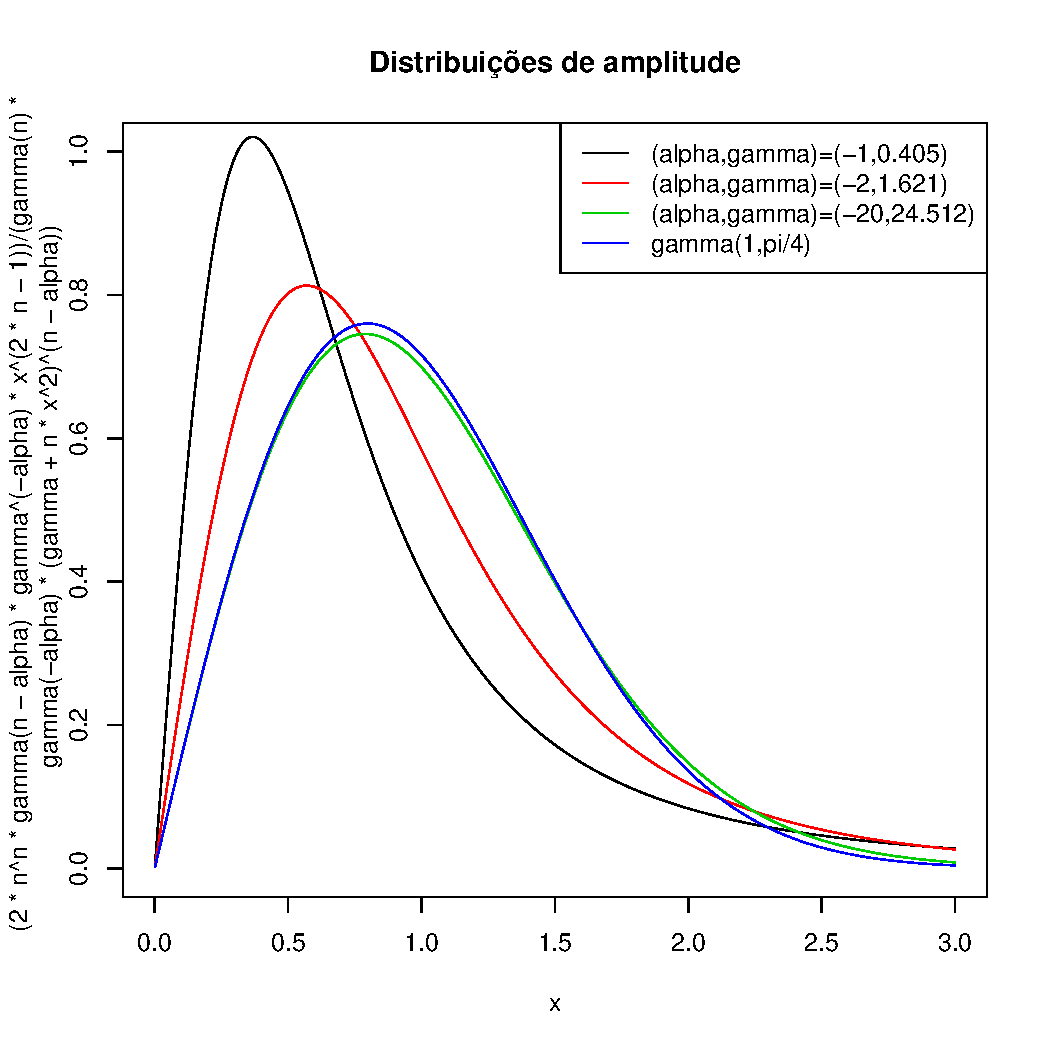
\includegraphics[width=4.0in]{fig_eq_ga_fig1_frery_muller_1997.pdf}
	\caption{Distribuições de amplitude.}
\label{fig11}
\end{figure}

\begin{figure}[!htb]
\centering
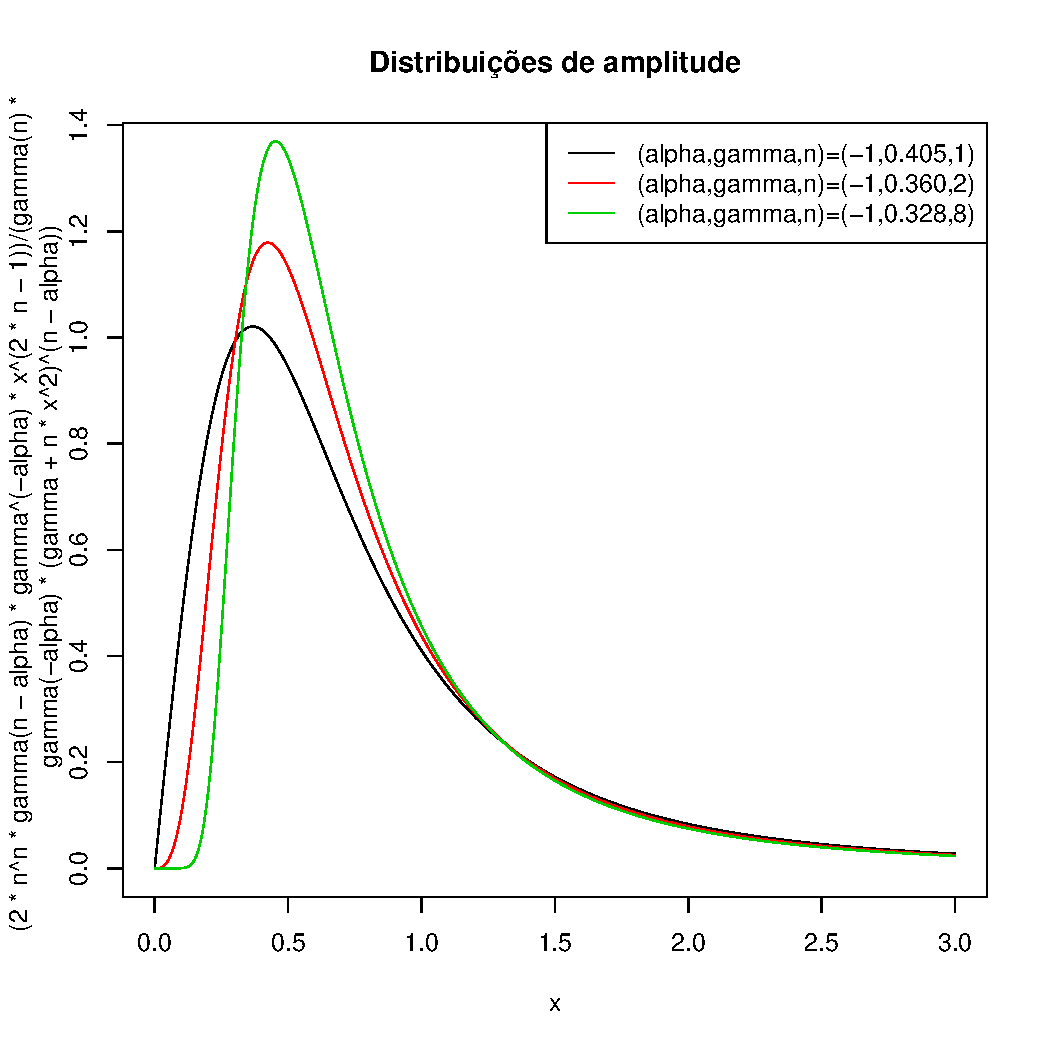
\includegraphics[width=4.0in]{fig_eq_ga_fig2_frery_muller_1997.pdf}
	\caption{Distribuições de amplitude.}
\label{fig12}
\end{figure}

\subsubsection{Modelando áreas urbanas}

Quando estimamos os três parâmetros da distribuíção $g_A$ sobre áreas urbanas foi observado que o atrator e a solução global do sistema de equações estava  no subconjunto do espaço de parâmetros dado por ($\alpha<0,\gamma0,\lambda<10^{-6}$); 


